%% This is the ctufit-thesis example file. It is used to produce theses
%% for submission to Czech Technical University, Faculty of Information Technology.
%%
%% Get the newest version from
%% https://gitlab.fit.cvut.cz/theses-templates/FITthesis-LaTeX
%%
%%
%% Copyright 2024, Tomas Novacek
%% Copyright 2021, Eliska Sestakova and Ondrej Guth
%%
%% This work may be distributed and/or modified under the
%% conditions of the LaTeX Project Public License, either version 1.3
%% of this license or (at your option) any later version.
%% The latest version of this license is in
%%  https://www.latex-project.org/lppl.txt
%% and version 1.3 or later is part of all distributions of LaTeX
%% version 2005/12/01 or later.
%%
%% This work has the LPPL maintenance status `maintained'.
%%
%% The current maintainer of this work is Tomas Novacek.
%% Alternatively, submit bug reports to the tracker at
%% https://gitlab.fit.cvut.cz/theses-templates/FITthesis-LaTeX/issues
%%
%%

% arara: pdflatex
% arara: biber
% arara: pdflatex
% arara: pdflatex

%%%%%%%%%%%%%%%%%%%%%%%%%%%%%%%%%%%%%%%%%
% CLASS OPTIONS
% language: czech/english/slovak
% thesis type: bachelor/master/dissertation
% colour: bw for black&white OR no option for default colour scheme
% electronic (oneside) or printed (twoside), twoside is default
%%%%%%%%%%%%%%%%%%%%%%%%%%%%%%%%%%%%%%%%%
\documentclass[english,bachelor,unicode,oneside,bw]{ctufit-thesis}

%%%%%%%%%%%%%%%%%%%%%%%%%%%%%%%%%%
% FILL IN THIS INFORMATION
%%%%%%%%%%%%%%%%%%%%%%%%%%%%%%%%%%
\ctufittitle{Application for configuration of modular products} % replace with the title of your thesis
\ctufitauthorfull{Michal Dobeš} % replace with your full name (first name(s) and then family name(s) / surname(s)) including academic degrees
\ctufitauthorsurnames{Dobeš} % replace with your surname(s) / family name(s)
\ctufitauthorgivennames{Michal} % replace with your first name(s) / given name(s)
\ctufitsupervisor{Ing.\,Jiří Hunka} % replace with name of your supervisor/advisor (include academic degrees)
\ctufitdepartment{Katedra softwarového inženýrství} % replace with the department of your defence
\ctufityear{2024} % replace with the year of your defence
\ctufitdeclarationplace{Prague} % replace with the place where you sign the declaration
\ctufitdeclarationdate{\today} % replace with the date of signature of the declaration
\ctufitabstractCZE{Fill in abstract of this thesis in Czech language.}
\ctufitabstractENG{Fill in abstract of this thesis in English language.}
\ctufitkeywordsCZE{enter, commma, separated, list, of, keywords, in, CZECH}
\ctufitkeywordsENG{enter, commma, separated, list, of, keywords, in, ENGLISH}
%%%%%%%%%%%%%%%%%%%%%%%%%%%%%%%%%%
% END FILL IN
%%%%%%%%%%%%%%%%%%%%%%%%%%%%%%%%%%

%%%%%%%%%%%%%%%%%%%%%%%%%%%%%%%%%%
% CUSTOMIZATION of this template
% Skip this part or alter it if you know what you are doing.
%%%%%%%%%%%%%%%%%%%%%%%%%%%%%%%%%%

\RequirePackage{iftex}[2020/03/06]
\iftutex % XeLaTeX and LuaLaTeX
    \RequirePackage{ellipsis}[2020/05/22] %ellipsis workaround for XeLaTeX
\else
    \RequirePackage[utf8]{inputenc}[2018/08/11] %this file encoding
    \RequirePackage{lmodern}[2009/10/30] % vector flavor of Computer Modern font
\fi

% hyperlinks
\RequirePackage[pdfpagelayout=TwoPageRight,colorlinks=false,allcolors=decoration,pdfborder={0 0 0.1}]{hyperref}[2020-05-15]

% uncomment the following to hide all hyperlinks
%\hypersetup{hidelinks}

% uncomment the following to change the colour of all hyperlinks to CTU blue
%\hypersetup{allbordercolors=decoration}

\RequirePackage{pdfpages}[2020/01/28]

%%%%%%%%%%%%%%%%%%%%%%%%%%%%%%%%%%
% CUSTOMIZATION of this template END
%%%%%%%%%%%%%%%%%%%%%%%%%%%%%%%%%%


%%%%%%%%%%%%%%%%%%%%%%
% DEMO CONTENTS SETTINGS
% You may choose to modify this part.
%%%%%%%%%%%%%%%%%%%%%%
\usepackage{dirtree}
\usepackage{lipsum,tikz}
\usepackage[style=iso-numeric]{biblatex}
\addbibresource{text/bib-database.bib}
\usepackage{listings} % typesetting of sources
%\usepackage[newfloat]{minted}\captionsetup[listing]{position=top} % typesetting of sources
\usepackage{csquotes}
\usepackage{todonotes}
\usepackage{textcomp}
\usepackage{pdflscape}

%%%%%%%%%%%%%%%%%%%%%%
% DEMO CONTENTS SETTINGS END
%%%%%%%%%%%%%%%%%%%%%%

\begin{document} 
\frontmatter\frontmatterinit % do not remove these two commands

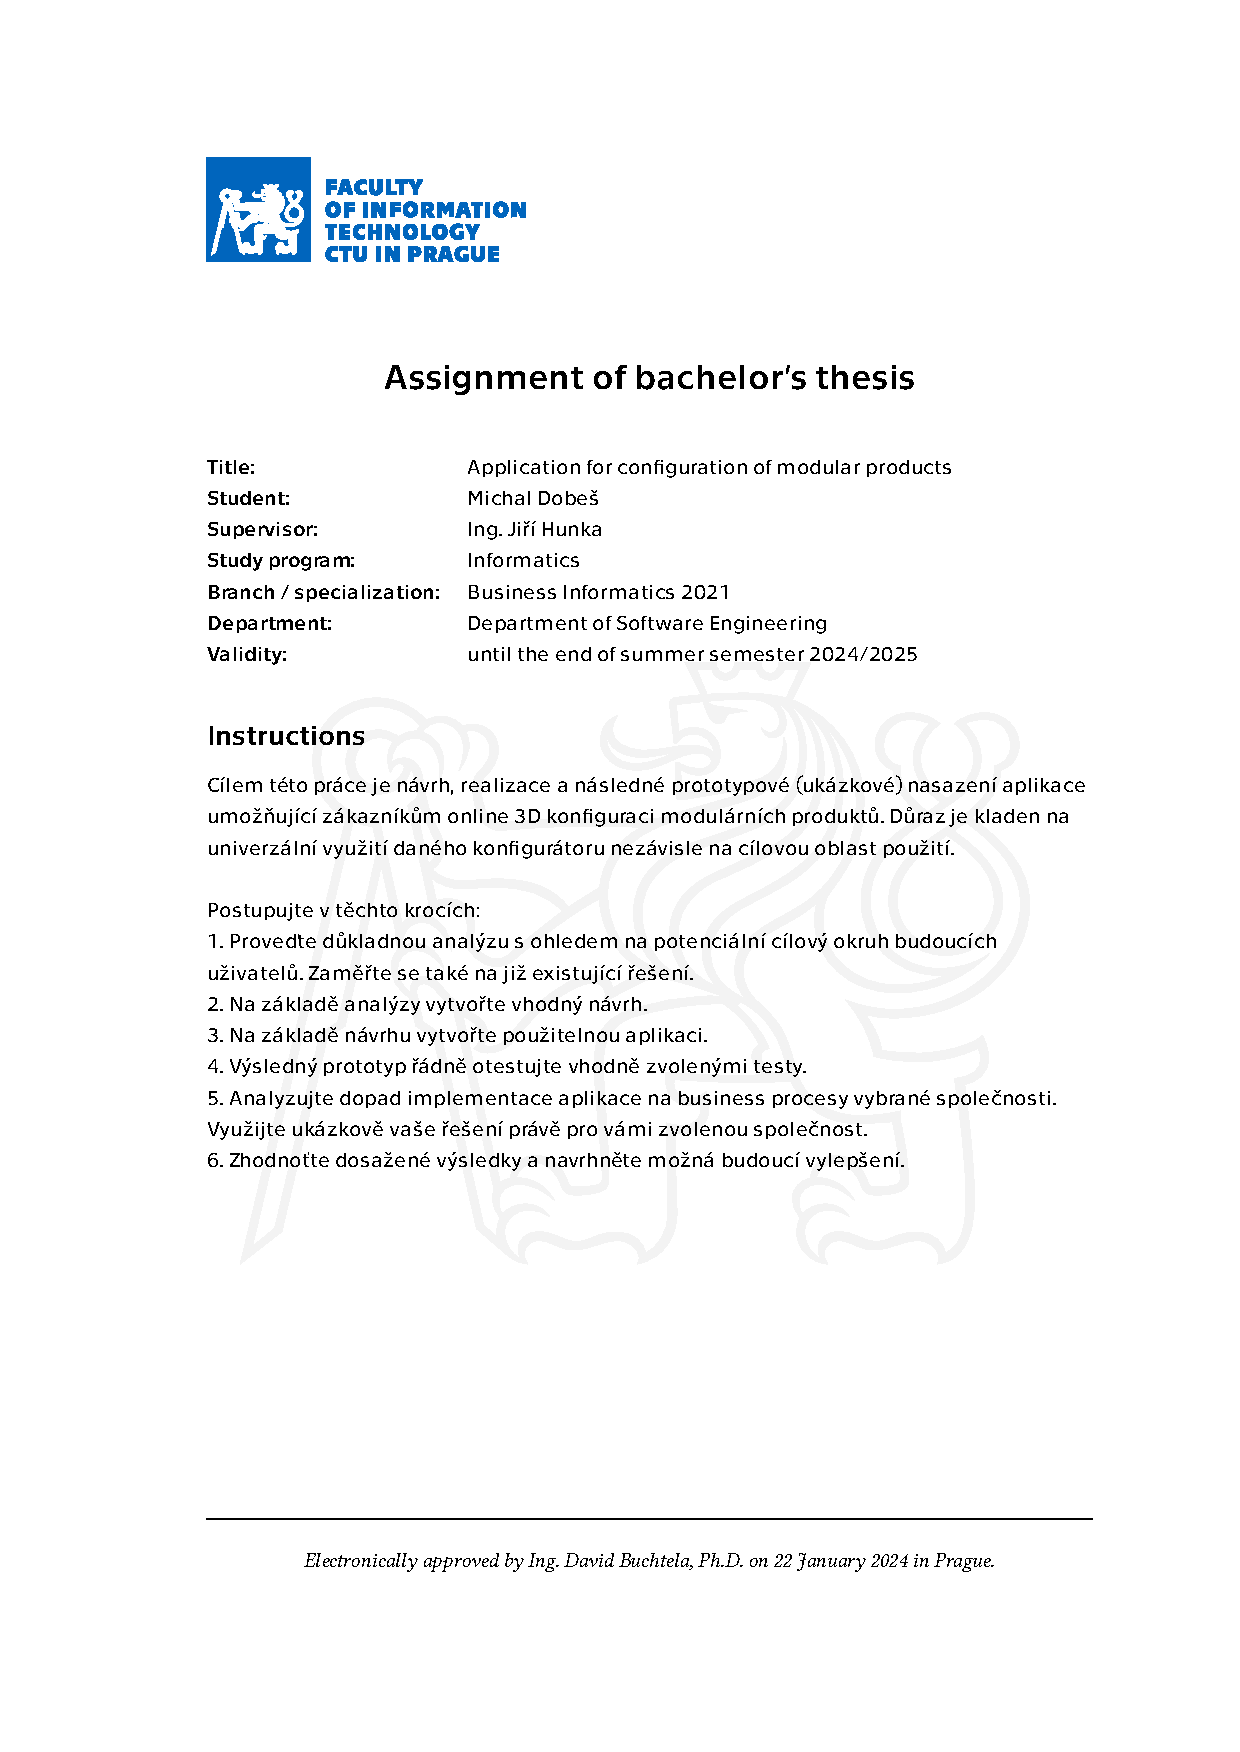
\includepdf[pages={1-}]{dobesmic-assignment.pdf} % replace that file with your thesis assignment provided by study office

\thispagestyle{empty}\cleardoublepage\maketitle % do not remove these three commands

\imprintpage % do not remove this command

\tableofcontents % do not remove this command
%%%%%%%%%%%%%%%%%%%%%%
% list of other contents: figures, tables, code listings, algorithms, etc.
% add/remove commands accordingly
%%%%%%%%%%%%%%%%%%%%%%
\listoffigures % list of figures
\begingroup
\let\clearpage\relax
\listoftables % list of tables
\thectufitlistingscommand
\endgroup
%%%%%%%%%%%%%%%%%%%%%%
% list of other contents END
%%%%%%%%%%%%%%%%%%%%%%

%%%%%%%%%%%%%%%%%%%
% ACKNOWLEDGMENT
% FILL IN / MODIFY
% This is a place to thank people for helping you. It is common to thank your supervisor.
%%%%%%%%%%%%%%%%%%%
\begin{acknowledgmentpage}
I would like to thank...
\end{acknowledgmentpage}
\todo{Fix heading of acnowledgements}
%%%%%%%%%%%%%%%%%%%
% ACKNOWLEDGMENT END
%%%%%%%%%%%%%%%%%%%


%%%%%%%%%%%%%%%%%%%
% DECLARATION
% FILL IN / MODIFY
%%%%%%%%%%%%%%%%%%%
% INSTRUCTIONS
% ENG: choose one of approved texts of the declaration. DO NOT CREATE YOUR OWN. Find the approved texts at https://courses.fit.cvut.cz/SFE/download/index.html#_documents (document Declaration for FT in English)
% CZE/SLO: Vyberte jedno z fakultou schvalenych prohlaseni. NEVKLADEJTE VLASTNI TEXT. Schvalena prohlaseni najdete zde: https://courses.fit.cvut.cz/SZZ/dokumenty/index.html#_dokumenty (prohlášení do ZP)
\begin{declarationpage}
FILL IN ACCORDING TO THE INSTRUCTIONS. VYPLNTE V SOULADU S POKYNY.
\end{declarationpage}
%%%%%%%%%%%%%%%%%%%
% DECLARATION END
%%%%%%%%%%%%%%%%%%%

\printabstractpage % do not remove this command

%%%%%%%%%%%%%%%%%%%
% SUMMARY
% FILL IN / MODIFY
% OR REMOVE ENTIRELY (upon agreement with your supervisor)
% (appropriate to remove in most theses)
%%%%%%%%%%%%%%%%%%%
% \begin{summarypage}
% \section*{Summary section}
% 
% \lipsum[1][1-8]
% 
% \section*{Summary section}
% 
% \lipsum[2][1-6]
% 
% \section*{Summary section}
% 
% \lipsum[3]
% 
% \section*{Summary section}
% 
% \lipsum[2]
% 
% \section*{Summary section}
% 
% \lipsum[1][1-8] Lorem lorem lorem.
% \end{summarypage}
%%%%%%%%%%%%%%%%%%%
% SUMMARY END
%%%%%%%%%%%%%%%%%%%

%%%%%%%%%%%%%%%%%%%
% ABBREVIATIONS
% FILL IN / MODIFY
% OR REMOVE ENTIRELY
% List the abbreviations in lexicography order.
%%%%%%%%%%%%%%%%%%%
\chapter{Abbreviations}
	
\begin{tabular}{rl}
AR & Augumented Reality\\
SPA & Single-Page Application\\
USDZ & Universal Scene Description Zip\\
API & Application Programming Interface\\
WebGL & Web Graphics Library\\
HTML & HyperText Markup Language\\
R3F & React Three Fiber\\
CSS & Cascading Style Sheets\\
\end{tabular}

\todo{Move all abbreviations from text here}
%%%%%%%%%%%%%%%%%%%
% ABBREVIATIONS END
%%%%%%%%%%%%%%%%%%%

\mainmatter\mainmatterinit % do not remove these two commands

%%%%%%%%%%%%%%%%%%%
% THE THESIS
%%%%%%%%%%%%%%%%%%%

% \chapter{Introduction}
% uncomment the following line to create an unnumbered chapter
\chapter*{Introduction}\addcontentsline{toc}{chapter}{Introduction}\markboth{Introduction}{Introduction}
\setcounter{page}{1}

% The following environment can be used as a mini-introduction for a chapter. Use that anyway it pleases you (or comment it out). It can contain, for instance, a summary of the chapter. Or, there can be a quotation.
\begin{chapterabstract}
Product configurators and their value.
\end{chapterabstract}
\todo{Update headlines to title-case}
Over the past few decades, the rise of e-commerce has caused a shift in consumer expectations, resulting in an increased demand for individualized products. This gives rise to the need to shift focus towards mass customization, where products are customized according to individual preferences. To thrive in this sector, companies must modify their product offerings to meet the unique needs of users. This necessitates the existence of a system that enables customers to express their preferences and convert them into product configurations. \cite{Fulkerson2000}

The task of transforming user preferences into concrete designs is a difficult endeavor that can be hindered by a lack of effective communication between the customer's explanation of their desires and the business's comprehension. The use of online product configurators seemingly provides a solution to this issue by offering a user-friendly and visually appealing platform that allows customers to customize products according to their specifications, improves the customer experience by increasing engagement and interactivity, and helps bridge the gap between customer expectations and the end product. These tools have become an integral part of successful personalization strategies. \cite{Franke2003}

The involvement of consumers in the customization process leads to a stronger bond with the product, resulting in a perception of a higher value of the product compared to standard off-the-shelf products. This aspect of mass customization makes it an appealing and compelling strategy for businesses to implement. \cite{Schreier2006} However, when implementing such a system, it is crucial to ensure that the customization process is pleasurable for the customer. Research has shown that the enjoyment experienced during the customization process also affects the perceived value of the final product, highlighting the importance of good implementation. \cite{Franke2010}

The introduction of modern technologies such as WebGL or Augmented Reality (AR) has expanded the potential of online configurators. These advances enable these toolkits to become more powerful and visually illustrative tools that provide a higher level of interactivity and realism than what was previously accessible. \cite{Cozzi2015}

%---------------------------------------------------------------
\section{Objective of this thesis}
%---------------------------------------------------------------

The primary objective of this thesis is to design and implement an application (toolkit) for the online configuration of modular products. The toolkit aims to be product-agnostic, adaptable, and customizable, usable by various businesses, enabling their customers to customize their modular products interactively. The focus is on ensuring that the toolkit is not only flexible in accommodating various specific needs, but also straightforward for businesses to maintain after deployment, emphasizing lightweight infrastructure requirements. 

To accomplish this main objective, an accompanying analysis of the characteristics found in current product configurators is required, as well as an examination of comparable solutions currently available to businesses.

%---------------------------------------------------------------
\section{Structure of this thesis}
%---------------------------------------------------------------

This thesis is divided into six chapters.

\begin{description}
\item[Chapter 1] The initial chapter entails an examination of existing solutions and an investigation into the functionalities that should be incorporated into this particular application.

\item[Chapter 2] The second chapter discusses the design of the application, the technologies chosen, the architecture, and the data structures.

\item[Chapter 3] The third chapter is devoted to implementation.

\item[Chapter 4] Chapter four focuses on the deployment of the implemented application in a particular business as an example. In addition, it discusses the resulting changes in the business processes of a chosen example business.

\item[Chapter 5] In the fifth chapter, the tests used in the development of the application are described.

\item[Chapter 6] Finally, the last chapter summarizes the results achieved and suggests possible directions for future development.
\end{description}
\chapter{Analysis}

\begin{chapterabstract}
A comprehensive evaluation of existing solutions, identification of key features and limitations, and outlining of the specifications for the proposed solution.
\end{chapterabstract}

Product configurators can be implemented in various ways, and the design of the tool itself determines the types of products that can be customized using the tool later on. The number of unique configurations of a product that the tool can create is called the solution space. The size of the solution space is determined by the count of customizable attributes and the achievable values of each attribute.~\cite{Huiwen2018} A relevant study examined the solution spaces of these toolkits and proposed an evaluation model that enables the categorization and assessment of various implementation approaches. Based on the target outcome and the guidance provided by the tool, the following mechanisms are defined:~\cite{Hermans2012}

\begin{definition}[Veneer]
Customization by adding a visual decorative layer. (e.g., printing, engraving, etching)
\end{definition}
\begin{definition}[Modularity]
Customization by combining modules or components.
\end{definition}
\begin{definition}[Parametric]
Customization by changing the parameter values of parts.
\end{definition}
\begin{definition}[Generative]
Customization using code and scripting to synthesize the final form of the product.
\end{definition}

There are often some common characteristics among configuration tools with different mechanisms; however, the main focus of this thesis is on toolkits that primarily employ modularity mechanisms.
\newpage

%---------------------------------------------------------------
\section{Existing Solutions}
%---------------------------------------------------------------
% - - - - - - - - - - - - - - - - - - - - - - - - - - - - - - -
\subsection{Applications of Product Configurators}
% - - - - - - - - - - - - - - - - - - - - - - - - - - - - - - -

Many companies across multiple industries, such as automotive, fashion, furniture, housing, are integrating product configurators into their sales strategies. These configurators serve as the main or supplementary sales tools for these businesses.

The Configurator Database Project by cyLEDGE MEDIA aims to catalog these web-based configuration tools. The 2017/2018 report tracked 1250 deployments of these tools; however, the true count will be significantly higher since the database only includes the most frequently visited applications.~\cite{cyLEDGE2018}

An analysis of the 100 most viewed configurators from May 2020 to May 2021 in the Configurator Database Project was performed in a study that examined the shared characteristics of these configurators.~\cite{Blazek2023} The summary of some of the relevant characteristics and design choices that the study has analyzed are presented in this section:
\begin{description}
    \item[Responsive design:] 75.3\% of examined tools had responsive design (the design adapted to the viewport of the device).
    \item[Navigation:] 17.5\% of configurators had linear predefined navigation (meaning the configuration had to follow a specified sequence), whereas the 82.5\% majority of tools had open navigation (meaning the user has the flexibility to configure the product in any order).
    \item[Visualization:] 79.4\% of tools utilized photorealistic visualization (as opposed to illustrations or no visualization); however, the study acknowledges that there were significant variations depending on the industries in which the configurator is utilized.
    \item[Data transfer:] The mean network data size transferred for 3D configurator was 35.6~MB.
    \item[Configuration options:] 60.8\% of configurators offered more than ten customizable attributes.
    \item[Purchase capability:] Given that car brands typically do not directly sell their cars online, they were excluded from the analysis of this particular characteristic. Without vehicle configurators, 70.5\% of the configurators could complete an online purchase of the configured product.
    \item[Price calculation:] 56.7\% of the configurators were able to instantly reflect the changes made to the configuration in the displayed price.
\end{description}

The previous paragraphs discussed general trends among all product configurators of all kinds. As part of the analysis in this chapter, it is essential also to examine existing modular 3D product configurators. 

Due to the large number of existing applications, it is not within the scope of this work to perform an exhaustive analysis. Instead, this section will focus on a select group of three applications. These have been selected based on a combination of factors such as their popularity, functionality, and importance in the context of a modular product configuration. This selection is intended to provide insightful examples that highlight different approaches, rather than being representative of the entire domain.

\noindent The main aspects under consideration are as follows:\nopagebreak
\begin{itemize}[label=\rectanglebullet]
    \item \textbf{Platform:} How is the application accessible?
    \item \textbf{Navigation:} How does the user navigate in the application during the configuration process?
    \item \textbf{Visualization style:} How is the product visualized within the configuration process?
    \item \textbf{Placement options:} Can the modular components be freely placed, or are they restricted to fixed points?
    \item \textbf{Camera movement:} From which angles can the product be visualized, and how can it switch between them? In the context of the tool, camera refers to a virtual camera in a 3D graphical environment that simulates the viewpoint and perspective from which the 3D scene is viewed.
    \item \textbf{Impossible configurations:} Is it possible to create configurations that are not feasible in reality?
    \item \textbf{Responsiveness:} How does the application adapt to different device viewports?
    \item \textbf{Price calculation:} Is the price of the configured product calculated in real-time?
    \item \textbf{Purchase option:} Is there an option to finalize and purchase the configured product within the application?
    \item \textbf{Save option:} Can users save their configurations to return to them later?
    \item \textbf{Version history:} Does the configurator provide an accessible history of configuration changes?
    \item \textbf{\noborderacrshort{vr} or \noborderacrshort{ar}:} Can the configured product be visualized in \noborderacrlong{vr} or \noborderacrlong{ar}?
    \item \textbf{Real dimensions}: Can the configurator display information about the real dimensions of the configured products? 
\end{itemize}
\break
\noindent Furthermore, the design decisions are also discussed:\nopagebreak
\begin{itemize}[label=\rectanglebullet]
    \item \textbf{Views:} What is the position and size of the views inside the application?
    \item \textbf{Navigation bars:} Where are the navigation bars placed and how are they utilized?
    \item \textbf{Button placements:} How are different buttons placed within the application's interface?
\end{itemize}


%______________________________________________________________
\subsubsection{IKEA PAX Planner}

IKEA is a widely recognized global home furnishings retailer specializing in affordable furniture.~\cite{StatistaIkea}

IKEA offers the PAX fitted wardrobe, for which they not only sell predefined configurations, but also allow customers to modularly choose the ideal size, doors, knobs, handles, interior organization, and lightning.~\cite{IkeaPAX}

To accomplish this, they utilize the PAX Planner web tool.\footnote{Available at: \url{https://www.ikea.com/addon-app/storageone/pax/web/latest/cz/en/}}

\begin{figure}[h]
\centering
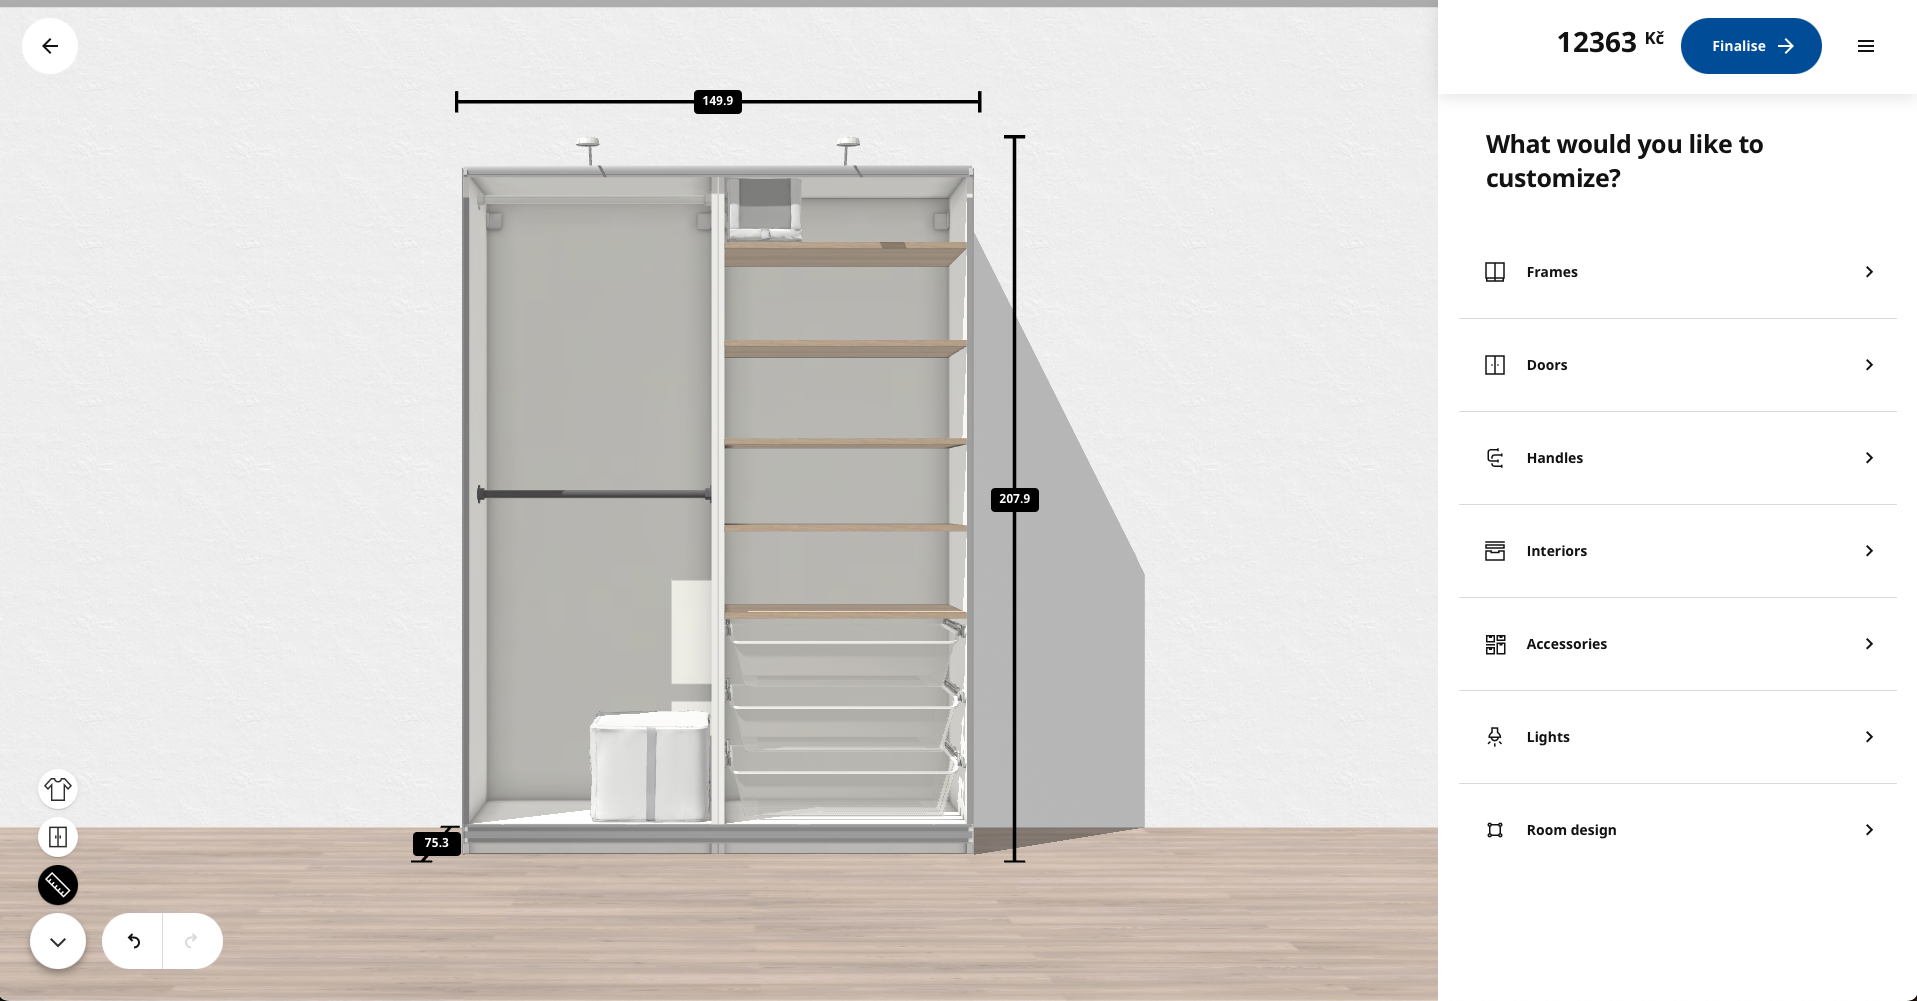
\includegraphics[width=\textwidth]{images/analysis_ikea-pax.png}
\captionsource{Screenshot of IKEA PAX Planner Tool with example configuration}{IKEA~\cite{IkeaPAX}}
\end{figure}

The tool consists mainly of two views. The primary view on the left contains a 3D preview of the configured product, allowing users to observe objects from different viewpoints by moving along an orbital trajectory in a 180-degree half-circle. The components displayed in the 3D view are both realistic and interactive. Users can adjust their position by dragging, and selecting a component offers additional information along with real-life images of the item. All modular options that can be added to the current configuration are found in the secondary smaller view on the right side and can be added by clicking or dragging them into the 3D preview. The application is responsive, and on mobile devices, the secondary view moves from the right side to a bottom sliding panel. The navigation bar is located at the top of the secondary view, and other buttons are located around the edges of the primary view.

At the beginning of the configuration process, the application prompts the user to select the starting point of the configuration. The configurator has open navigation, meaning that the components can then be configured in any order. Components can be placed anywhere along a specified axis with certain restrictions, effectively preventing the creation of impossible configurations.

The tool performs live price calculations and contains a final summary confirmation screen from which it is possible to order the configured product in the e-shop. The configurator maintains a history of recent changes, accessible through undo and redo buttons. It also features the ability to save configurations on the server, which can be retrieved later using a generated code.

The configurator also provides a range of innovative features, such as the ability to change the visibility of some elements using a button (e.g. hiding the doors of a wardrobe to reveal the contents inside) or the ability to display dimensions directly in the 3D preview.

The application is a \noborderacrfull{spa} and does not update the \noborderacrshort{url} based on the selected product or phase of the configuration.

\noborderacrshort{spa} is a web application implementation approach that loads only a single page and then sequentially updates the content of the page with scripting on the client side, rather than loading whole new pages from the server.~\cite{Fink2014}


%______________________________________________________________
\subsubsection{Muuto Product Planner}

Muuto is a Scandinavian design company that produces furniture and home accessories. \cite{Muuto}

The company provides Product Planner, a 3D web-based configurator, which allows customers to customize and combine the designs of various products, such as storage systems, sofas, tables, or wall hangers, tailored to their specific needs.\footnote{Available at: \url{https://planner.muuto.com/}}~\cite{MuutoPlanner}

\begin{figure}[h]
\centering
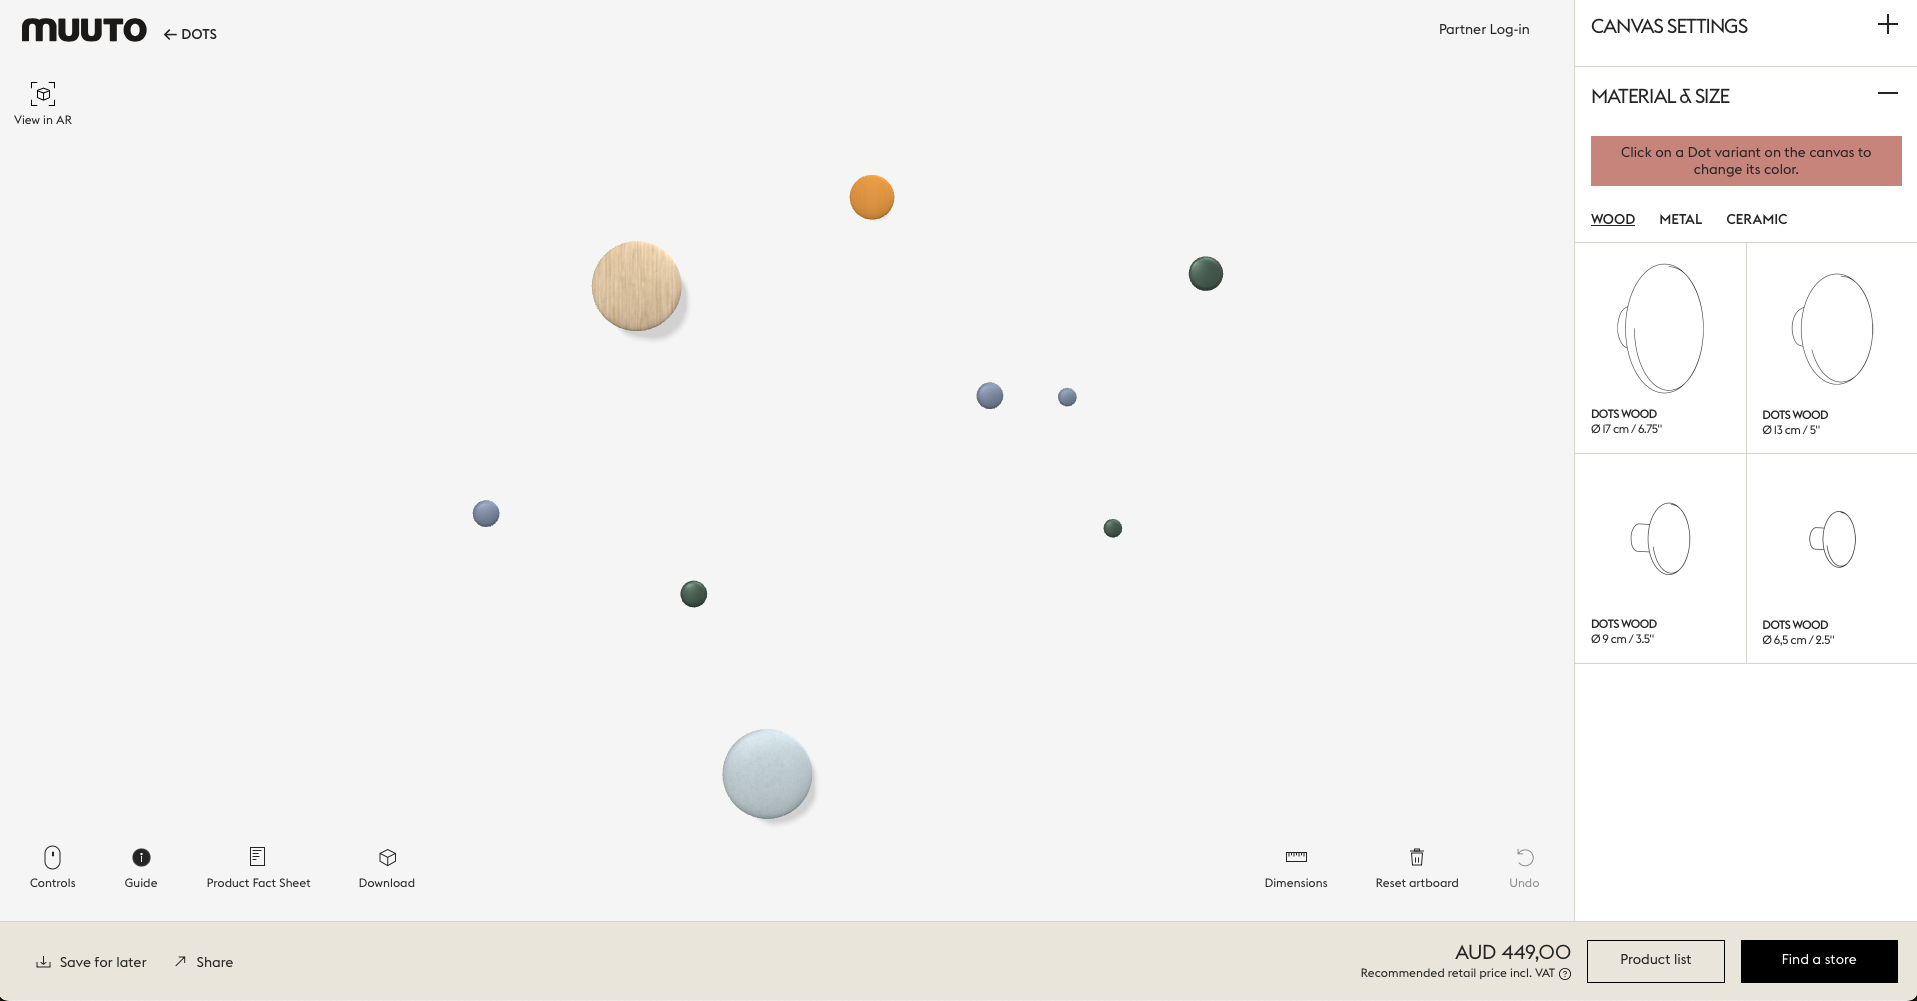
\includegraphics[width=\textwidth]{images/analysis_muuto-product-planner.png}
\captionsource{Screenshot of Muuto Product Planner tool with example configuration}{Muuto~\cite{MuutoPlanner}}
\end{figure}

The design of the configurator is similar to that in the previous case. The configurator also consists of two views. The primary view on the left provides full realistic 3D visualization, while the smaller secondary view on the right side allows users to add components by dragging them into the main view. Selecting a component in the primary view enables users to remove it or alter its materials. As the design is responsive, on smaller devices, the secondary view transforms into a bottom slide panel. Depending on the configured product, the tool offers a preview either from a single angle or a preview from any point on an orbital trajectory. The main view is also surrounded by buttons along its edges. The navigation bar is positioned at the bottom across the entire application, while the company logo is displayed on the top left.

The tool follows a similar flow, starting with the selection of the starting point and then moving to the configurator process, which has open navigation. Components can be placed anywhere, unless their position is dependent on another component. Due to this flexibility and also the wide variety of products that it supports, the configurator is not restricted to generating configurations that are feasible to produce and can create impossible configurations.

The tool can display real dimensions and can reverse the performed changes using the undo and redo buttons. The configuration can also be saved on the server-side and later accessed using a unique code. Live price calculation is also performed, and there is a summary page, but it is not possible to order the configured product; instead, the user is redirected to a physical store locator.

Furthermore, the designed configuration can be quickly shared with other users using email, or it can be downloaded in several file formats containing the 3D model itself. The application makes it possible to view the product in \noborderacrshort{ar}, directly in a web browser, albeit only on Apple devices using the \noborderacrfull{usdz} format and \noborderacrshort{ar}~Quick Look.~\cite{Jackson2018}

The application has multiple URL schemes that depend on the configuration phase, but they are not determined by the current product. 

%______________________________________________________________
\subsubsection{LD Seating Nido Configurator}

LD Seating is a company based in the Czech Republic that specializes in the production of chairs, armchairs, and sofas.~\cite{LDSeating}

The company uses a 3D web-based configurator to market the Nido modular seating system, which consists of elements that are designed to be combined in various ways.\footnote{Available at: \url{https://nido.ldseating.com/en/configurator}}~\cite{NidoConfigurator}

\begin{figure}[ht]
\centering
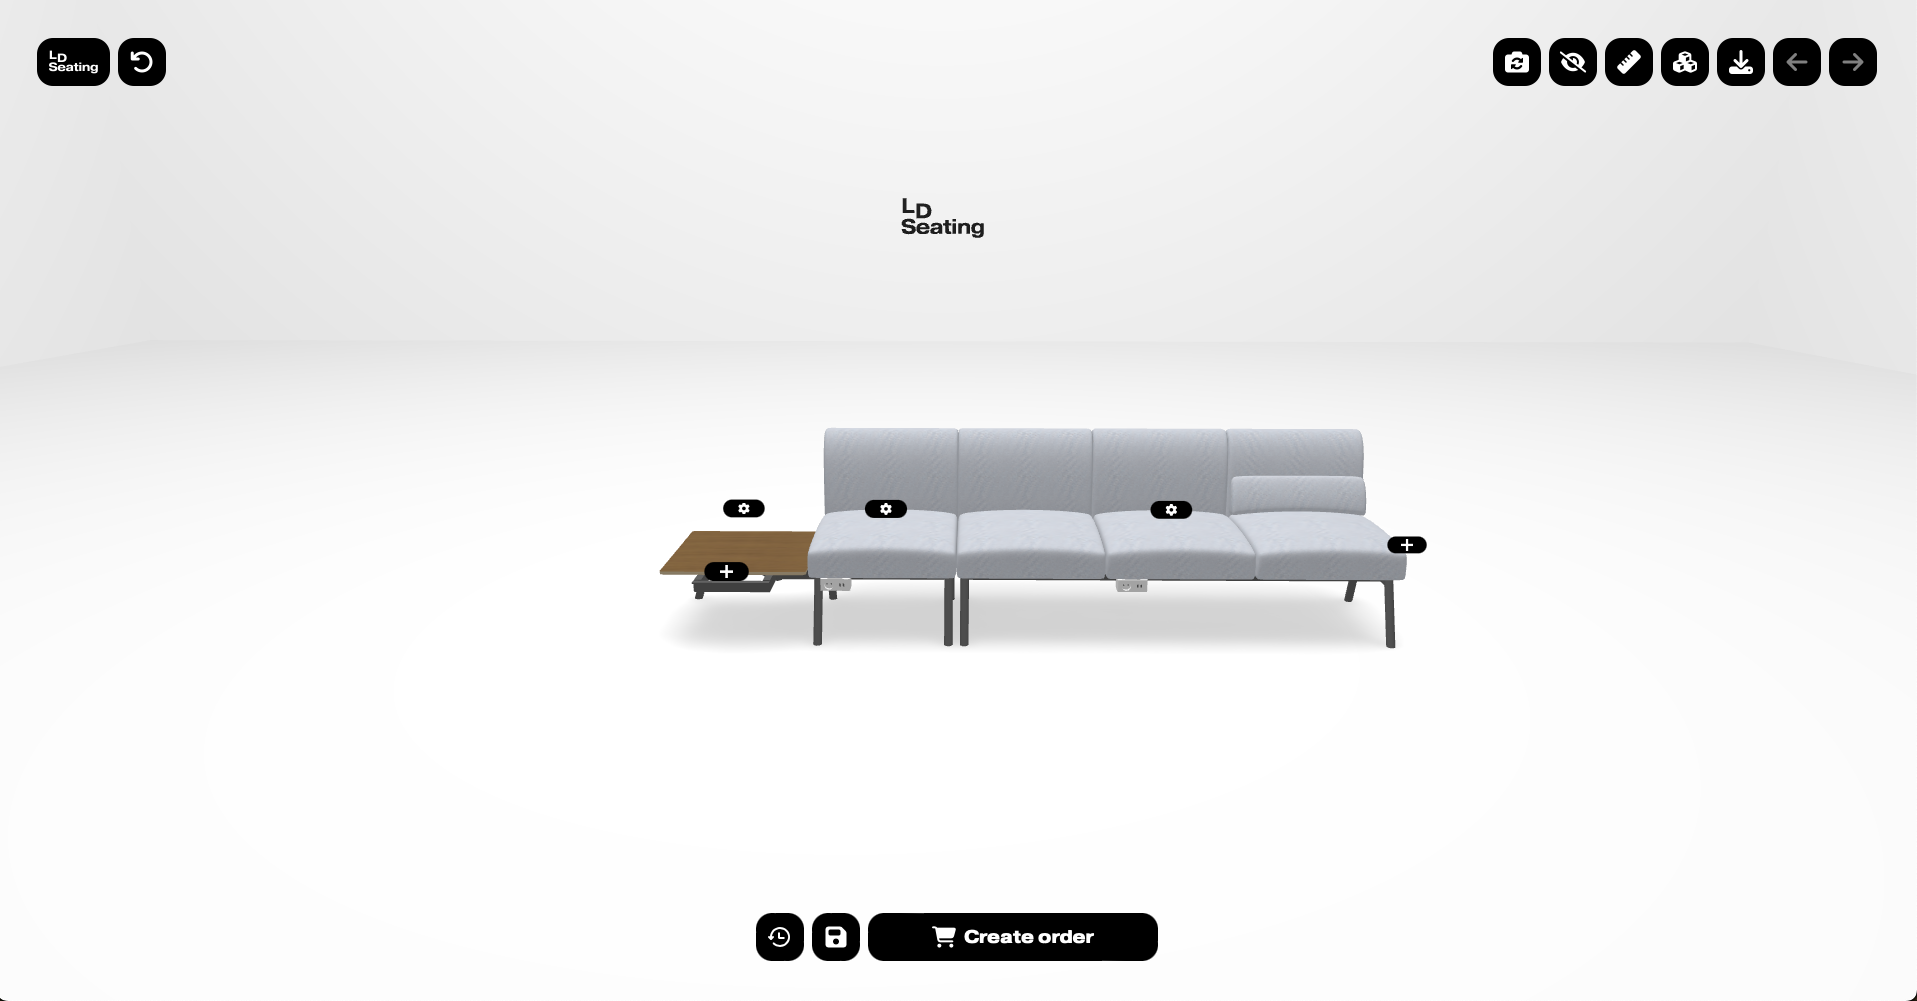
\includegraphics[width=\textwidth]{images/analysis_nido-configurator.png}
\captionsource{Screenshot of LD Seating Nido Configurator with example configuration}{LD Seating~\cite{NidoConfigurator}}
\end{figure}

The configurator consists of one large view, covering the whole application, which displays high-definition 3D models of the configured components. The buttons are placed around the entire view, on the top right, bottom center, and top left, where the company logo is also displayed.  The controls for adding components and modifying properties are embedded directly in the 3D scene. When necessary, a panel opens to the right, allowing users to select components to add, adjust component properties, or change materials. The application is partially responsive, as the side panel opens fullscreen on smaller viewports; however, there are some issues with image and text overflows on mobile devices. The main view allows the user to observe the configuration from all angles along an orbital trajectory.

The flow of the application also includes selecting a starting point. The product configuration process itself uses open navigation. The tool assesses whether a component can fit into a space and, if not, prevents its placement, thereby restricting impossible configurations. At the completion of the configuration, a confirmation summary is presented; however, in this case, the price is not calculated live. The configurator cannot directly place an order for the product, but instead confirming results in the display of an inquiry form.

The resulting configuration can be downloaded as a file containing the 3D models. The configuration can also be saved server-side, which generates a unique link at which the configuration is accessible. The tool features a version history that stores each saved configuration for future access. Users can revisit these versions, while undo and redo buttons are also available. The resulting configuration can also be exported to a \noborderacrshort{pdf} file containing a list of components. The tool also has the ability to display real dimensions.

The application is a \noborderacrshort{spa}, maintaining a consistent \noborderacrshort{url} and changing it to reflect the location of a saved configuration (if one exists).


% - - - - - - - - - - - - - - - - - - - - - - - - - - - - - - -
\subsection{Available Toolkits}
% - - - - - - - - - - - - - - - - - - - - - - - - - - - - - - -

In this section of the analysis chapter, the focus shifts from specific 3D modular configurator applications to the fundamental toolkits that power the configurators. Although many configurators are bespoke and tailored to the specific needs of companies and their individual products, there are providers offering more generic and adaptable solutions. These offerings are highly relevant to this thesis, as the objective of this thesis is to create a product-agnostic toolkit, which means that there is a need to consider the way the configurator is set up by the business.

A variety of providers offer these toolkits for deploying product configurators, intending to provide semi-custom or fully custom solutions, as well as generic options. This section examines two particular toolkits to carry out a focused and relevant analysis. The choice of toolkits analyzed has been complicated by the fact that most providers are cautious about the details of the technology, typically revealing in-depth information only after a serious business inquiry. The choice was also based on factors such as the implementation approach and compatibility with modular products.

\noindent This section seeks to answer the following questions about the toolkits: 
\begin{itemize}[label=\rectanglebullet]
    \item \textbf{Administration}: How is the product configurator created and administered?
    \item \textbf{Assets}: How are assets stored and cataloged?
    \item \textbf{Product configuration}: How are the configuration options and rules defined?
    \item \textbf{Integration}: How is the tool integrated into other systems?
    \item \textbf{Pricing}: What is the cost of the offered solution?
\end{itemize}


%______________________________________________________________
\subsubsection{Threekit}

Threekit is a leading global company in visual commerce technologies that specializes in 3D product visualizations. The Threekit Platform, which enables clients to create interactive product experiences according to their needs, functions as an administrative application and has the capability to generate product configurators (see \autoref{fig:threekit-platform} in \autoref{appendix-a}).~\cite{ThreeKitAboutUs, ThreeKitPlatform}

The platform is very complex with many distinct features. At its core, it uses a catalog for storing all product data (the products themselves, materials used, configurable parts, etc.). The items in the catalog can then be loaded into The Treekit Player, which will display the models in 3D, with the option for users to change attributes (models and materials) that are tied to the item. The behavior of the configurator can be set up using item rules and logic that support conditions, queries, and even custom scripts. The platform also offers a data tables feature that is similar to spreadsheets and is designed to handle extensive configuration data and logic. The application also has a built-in asset editor for refining 2D and 3D assets and configuration options (see \autoref{fig:threekit-editor} in \autoref{appendix-a}). Models of the products can be uploaded in various 3D formats. The platform provides \noborderacrshort{api} integration with the leading e-commerce and \noborderacrshort{erp} systems.~\cite{ThreeKitPlatformDocumentation}

The offered solution is still partially tailored to the client, which is the reason why the service does not have standardized pricing. Instead, the price is determined through a personalized quote. It is important to note that the analysis of Threekit presented here is based on the publicly available documentation of the platform. Direct access to the full suite of Threekit's tools is typically available only after formalizing a business agreement with the company.


%______________________________________________________________
\subsubsection{Roomle}

Roomle is an Austrian company focused on pioneering visual product configuration. They provide solutions for product visualization, room design, and product configurators. Roomle's solution, called Rubens, is described as a \enquote{Open Full Logic 3D-Configurator}. The tool utilizes both parametric and modular configuration mechanisms. The software allows integration with third parties through the use of an \noborderacrshort{api}. In addition, it supports integration with other front-end technologies on web and mobile platforms and has a built-in \noborderacrshort{ar} experience.~\cite{RoomleAbout}

A web application, Rubens Admin, is used to set up the configurator application. To add a product that can then be configured by customers, 3D models, and materials are uploaded to the admin application. Components are defined using RoomleScript language, which is loosely based on the JavaScript language. The design of the configurator itself can be tuned in the admin application as well. Multiple language variants can be defined for product names and descriptions. The configurator application (see \autoref{fig:roomle} in \autoref{appendix-a}) runs on the client-side and can be simply embedded into a website. Additionally, a JavaScript library that can subscribe to events or modify the configurator can be utilized. A framework is also provided to utilize the configurator within an iOS application.~\cite{RoomleDocumentation}

In terms of pricing, Roomle's Rubens configurator with the listed capabilities is offered to businesses at a monthly fee of €1450.~\cite{RoomleFullLogic}

% - - - - - - - - - - - - - - - - - - - - - - - - - - - - - - -
\subsection{Summary of Existing Solutions}
% - - - - - - - - - - - - - - - - - - - - - - - - - - - - - - -

\begin{table}[htb!]
\centering
\begin{tabular}{>{\raggedright\arraybackslash}p{3.8cm}*{3}{>{\centering\arraybackslash}p{2.5cm}}} 
\toprule
\parbox[c][7ex]{3.8cm}{\textbf{Features}} &
\multrow{c}{\textbf{IKEA} \\ \textbf{Pax} \\ \textbf{Planner}} &
\multrow{c}{\textbf{Muuto} \\ \textbf{Product} \\ \textbf{Planner}} &\multrow{c}{\textbf{LD Seating} \\ \textbf{Nido} \\ \textbf{Configurator}} \\ 
\midrule
\parbox[c][7ex]{3.8cm}{Platform}
    & Web
    & Web
    & Web \\ 
\parbox[c][7ex]{3.8cm}{Navigation}
    & Open
    & Open
    & Open \\ 
\parbox[c][7ex]{3.8cm}{Visualization}
    & Realistic
    & Realistic
    & Realistic \\ 
\parbox[c][7ex]{3.8cm}{Placement options}
    & Free
    & Free
    & Fixed points\\ 
\parbox[c][7ex]{3.8cm}{Camera movement}
    & Orbital
    & \multrow{c}{Orbital; \\ Static}
    & Orbital \\
\parbox[c][7ex]{3.8cm}{Impossible \\ configurations} 
    & No
    & Yes
    & No \\
\parbox[c][7ex]{3.8cm}{Responsiveness}
    & Yes
    & Yes
    & Yes \\
\parbox[c][7ex]{3.8cm}{Price calculation}
    & Yes
    & Yes
    & No \\
\parbox[c][7ex]{3.8cm}{Purchase option}
    & E-shop order
    & Store locator
    & Inquiry form \\
\parbox[c][7ex]{3.8cm}{Save option}
    & Server-side
    & \multrow{c}{Server-side; \\ Local}
    & \multrow{c}{Server-side; \\ Local} \\
\parbox[c][7ex]{3.8cm}{Version history}
    & Undo \& redo 
    & Undo \& redo
    & \multrow{c}{Undo \& redo; \\ Multiple saves} \\
\parbox[c][7ex]{3.8cm}{VR or AR}
    & No
    & Yes
    & No \\
\parbox[c][7ex]{3.8cm}{Real dimensions}
    & Yes
    & Yes
    & Yes \\
\bottomrule
\end{tabular}
\caption{Summary of key points discussed in the analysis of existing modular product configurators}
\label{table:summary-analysis}
\end{table}

All the product configurators analyzed have common characteristics, especially in terms of navigation and visualization styles, which remain consistent across different tools. Despite this, certain trade-offs were observed between them, especially regarding placement options. While some solutions offer users the freedom to position components anywhere, others restricted placement to fixed points. This variance stems from implementation complexity, as the fixed-point system is simpler, furthermore offering a better way to restrict impossible configurations.
Another significant distinction was observed in the product finalization process, which ranged from the ability to place an order to being directed to a physical store.

The key points discussed in the analysis of modular product configurators are summarized in \autoref{table:summary-analysis}.

The user interface design of the analyzed configurations also displayed similarities, particularly in layout style, featuring a primary 3D preview on the left, a secondary view on the right, and buttons surrounding the primary view.

Analyzing the offered toolkit solutions proved challenging due to the information being closely guarded, as it is in the financial interest of the providers. However, the examined toolkits are very sophisticated solutions that are supported by large backend services, which are used for storing assets and facilitating the configurators functionality. The toolkits offer advanced features that allow for the definition of rules and logic, allowing companies to create configurators with a large amount of complexity. This indicates that these toolkits target a market composed mainly of larger corporations that require sophisticated solutions, which is also reflected in pricing.

%---------------------------------------------------------------
\section{Proposed Solution}
%---------------------------------------------------------------

This thesis aims to develop a new solution for the configuration of modular products. To do so, the proposed solution will incorporate the common characteristics identified in the analyzed solutions. The following paragraphs of this chapter should answer the important questions of who, what, why and how, detailing the key aspects of the proposed solution. 

The main differentiation factor of this proposed toolkit is its emphasis on catering to small businesses. As the existing toolkits that were examined were costly and mainly aimed at larger companies, this solution aims to fill this market gap. To achieve this, it will be necessary to make some trade-offs ensuring the solution's adaptability and relevance across various product types without making the solution overly complex. Therefore, the proposed toolkit will prioritize simplicity and cost-effectiveness, following the best practices seen in larger-scale solutions but with a specific focus on the needs and capabilities of the target market.

The following chapter outlines the features that should be implemented in the solution proposed in this thesis.
 
The proposed toolkit is envisioned to be universal with regard to products, adaptable, and customizable, catering to a wide variety of modular products and industries. The solution should be simple for businesses to deploy and manage, without the need for extensive technical resources, ensuring that it is straightforward for smaller businesses to maintain and operate effectively.

% - - - - - - - - - - - - - - - - - - - - - - - - - - - - - - -
\subsection{Requirement Engineering} \label{section:requirements}
% - - - - - - - - - - - - - - - - - - - - - - - - - - - - - - -

Following the overview of objectives and the definition of the target market, it is necessary to formulate precise requirements for this solution. Detailing these features and characteristics is crucial for successful implementation. Thus, the description of requirement engineering for this solution will be provided here.

The process of requirement engineering for software products involves gathering, analyzing, selecting, and managing requirements. It focuses on interpreting and understanding the goals, needs, and beliefs of stakeholders and transforming them into specific requirements.~\cite{Aurum2005}

There are many ways to categorize software requirements, such as audience-oriented categorization or using the FURPS method, which classifies requirements based on functionality, usability, reliability, performance, or supportability.~\cite{Stephens2023}

Given that the majority of requirements for the solution fall either into the functionality or usability category, the requirements in this section are separated only into the following two main categories:~\cite{Aurum2005}
\begin{enumerate}
    \item Functional requirements: These requirements describe what the system should be able to do. They specifically outline the system's behavior and its interactions in specific situations.
    \item Non-functional requirements: These requirements put constraints on the solution that meets the functional requirements, rather than being focused on specific behaviors of the system. They are often, among others, focused on performance, security, accessibility, and compatibility.
\end{enumerate}

To manage and prioritize these requirements, each is assigned an approximate priority level using the MoSCoW method. This approach classifies the requirements into four distinct categories:~\cite{Stephens2023}
\begin{enumerate}
    \item Must: Requirements crucial for the final solution.
    \item Should: Requirements to be implemented if feasible.
    \item Could: Requirements that are desirable but not essential.
    \item Won't: Nice-to-have requirements that most likely will not be implemented in this solution.
\end{enumerate}
This method helps to plan and allocate resources throughout the implementation phase.

\break
Additionally, each requirement is given a rough estimate of the implementation difficulty, separated into three categories: \nopagebreak
\begin{enumerate}
    \item Simple: Requirements that are straightforward to implement and require little time and few resources.
    \item Intermediate: Requirements that pose moderate challenges and demand a considerable amount of resources, time, and problem-solving.
    \item Complex: Requirements that are highly challenging and involve substantial resources, time, and expertise.
\end{enumerate}
This preliminary assessment aims to classify the requirements without relying on specific rigid criteria for each category. This method is specifically used only for functional requirements, as non-functional requirements affect the software's functionality and user experience through abstract constraints, making them unsuitable for the same difficulty estimation approach.
% - - - - - - - - - - - - - - - - - - - - - - - - - - - - - - -
\subsubsection{Functional Requirements}
% - - - - - - - - - - - - - - - - - - - - - - - - - - - - - - -

\begin{enumerate}[label=\textbf{F\arabic*:}, leftmargin=*]
\item \label{itm:F1} 3D product visualization
\vspace{2pt}
\\The tool shall offer users 3D visualization of their configured product, employing realistic models to accurately represent the components used and their characteristics.
\begin{itemize}[noitemsep, label=\trianglebullet]
    \item \textbf{Priority:} Must
    \item \textbf{Difficulty:} Complex
\end{itemize}
\vspace{4pt}

\item \label{itm:F2} Dynamic orbital camera controls
\vspace{2pt}
\\The tool should have dynamic orbital camera controls that allow users to view the product in the 3D product visualization (see requirement \hyperref[itm:F1]{F1}) from any angle by rotating, panning, and zooming the camera around the product. This feature aims to provide an engaging visual experience that allows users to examine the product with a 360-degree view. The controls should be intuitive, allowing for seamless navigation through mouse actions or touch gestures depending on the device used.
\begin{itemize}[noitemsep, label=\trianglebullet]
    \item \textbf{Priority:} Must
    \item \textbf{Difficulty:} Simple
\end{itemize}
\vspace{4pt}

\item \label{itm:F3} Modularity configuration mechanism
\vspace{2pt}
\\The toolkit should incorporate modularity mechanisms that allow users to configure products by adding, removing, or modifying components within the overall product or in relation to other components. Different modules may be available for each component, and the toolkit administrator should have the ability to designate them either as optional or mandatory, \phantom{thereby enhancing the flexibility of configuration.}\newpage thereby enhancing the flexibility of configuration.
\begin{itemize}[noitemsep, label=\trianglebullet]
    \item \textbf{Priority:} Must
    \item \textbf{Difficulty:} Intermediate
\end{itemize}
\vspace{4pt}

\item \label{itm:F4} Component interactivity
\vspace{2pt}
\\The configurator should support interactivity with each component of the product. Users should be able to select components directly within the 3D visualization (see requirement \hyperref[itm:F1]{F1}), which should allow them to change attributes of the components, remove them, or swap them with alternative options (see requirement \hyperref[itm:F3]{F3}). The changes made by the users should be immediately visible, allowing for an iterative and engaging customization process. Moreover, the components that are interacted with need to offer feedback, such as highlighting, in order to assist users in navigating the accessible customization choices.
\begin{itemize}[noitemsep, label=\trianglebullet]
    \item \textbf{Priority:} Should
    \item \textbf{Difficulty:} Complex
\end{itemize}
\vspace{4pt}

\item \label{itm:F5} Open navigation
\vspace{2pt}
\\The configurator should offer high flexibility in the order of configuring components and attributes, avoiding a linear step-by-step configuration and enabling all changes to be performed at any point during the configuration process. This flexibility enhances the user's ability to navigate freely among various different components of the product (see requirement \hyperref[itm:F3]{F3}).
\begin{itemize}[noitemsep, label=\trianglebullet]
    \item \textbf{Priority:} Should
    \item \textbf{Difficulty:} Simple
\end{itemize}
\vspace{4pt}

\item \label{itm:F6} Fixed point component placement
\vspace{2pt}
\\In alignment with the modularity configuration mechanism (see requirement \hyperref[itm:F3]{F3}), the configurator should enable components to be attached to other components or the whole product at predefined fixed points. While this approach restricts the potential solution space, it greatly streamlines the configuration process from the user side and helps to ensure that the configured product remains within the realm of feasible configurations.
\begin{itemize}[noitemsep, label=\trianglebullet]
    \item \textbf{Priority:} Should
    \item \textbf{Difficulty:} Intermediate
\end{itemize}
\vspace{4pt}

\item \label{itm:F7} Component collision detection
\vspace{2pt}
\\The tool should incorporate a collision detection system to prevent components from being positioned in such a way that would result in physical overlaps during configuration. This feature is essential to maintain \phantom{the realism and feasibility of the configured product.}\newpage the realism and feasibility of the configured product.
\begin{itemize}[noitemsep, label=\trianglebullet]
    \item \textbf{Priority:} Should
    \item \textbf{Difficulty:} Complex
\end{itemize}
\vspace{4pt}

\item \label{itm:F8} Material color configuration
\vspace{2pt}
\\Users should be able to modify the appearance of materials of components and products through a selection from a palette of colors. The chosen appearance should immediately be reflected in the 3D visualization (see requirement \hyperref[itm:F1]{F1}) of the configuration.
\begin{itemize}[noitemsep, label=\trianglebullet]
    \item \textbf{Priority:} Should
    \item \textbf{Difficulty:} Complex
\end{itemize}
\vspace{4pt}

\item \label{itm:F9} Configuration review
\vspace{2pt}
\\Before the configuration process is finalized, users should be presented with a review page that allows for a detailed examination of their product configuration. This feature should provide a summary listing all selected components and any other parameters. In addition, users should be able to return to previous configuration steps to make any necessary adjustments.
\begin{itemize}[noitemsep, label=\trianglebullet]
    \item \textbf{Priority:} Should
    \item \textbf{Difficulty:} Simple
\end{itemize}
\vspace{4pt}

\item \label{itm:F10} Configuration processing
\vspace{2pt}
\\At the end of the configuration process, users should be optionally presented with a confirmation button, provided that a specific confirmation action has been set up for the product. This button is intended for users to confirm their choices and trigger a predetermined action, such as calling a webhook or being directed to another page, as specified by the administrator. This should allow for a smooth transition, where, upon configuration confirmation, the user is engaged in a follow-up action, like a checkout process or being guided to a physical store locator page. The ability to perform a custom \noborderacrshort{api} call at the end of the configuration process provides a flexible way to integrate the configurator with different systems or processes, thus improving its functionality and delivering a seamless user experience from start to finish.
\begin{itemize}[noitemsep, label=\trianglebullet]
    \item \textbf{Priority:} Should
    \item \textbf{Difficulty:} Simple
\end{itemize}
\vspace{4pt}

\item \label{itm:F11} Inquiry form
\vspace{2pt}
\\As an extension of configuration processing (see requirement \hyperref[itm:F10]{F10}), the administrator should be able to set the product's confirmation action to trigger an inquiry form. In this scenario, when users click on the confirmation button, they should encounter a form asking for their contact details. Once completed, the created product configuration along with the user's contact information should be sent to an \noborderacrshort{api} predefined by the toolkit's administrator. This allows for a standard inquiry form process directly within the configurator application.
\begin{itemize}[noitemsep, label=\trianglebullet]
    \item \textbf{Priority:} Should
    \item \textbf{Difficulty:} Simple
\end{itemize}
\vspace{4pt}

\item \label{itm:F12} Configuration saving and retrieval
\vspace{2pt}
\\The tool should allow users to save the current product configuration, allowing them to pause the customization process without losing progress. Users should have the ability to easily access and resume editing their saved configurations at a later time.
\begin{itemize}[noitemsep, label=\trianglebullet]
   \item \textbf{Priority:} Could
    \item \textbf{Difficulty:} Intermediate
\end{itemize}
\vspace{4pt}

\item \label{itm:F13} Undo and redo actions
\vspace{2pt}
\\The configurator should integrate undo and redo functionality, enabling users to easily revert or reapply changes made anytime during the configuration process.
\begin{itemize}[noitemsep, label=\trianglebullet]
    \item \textbf{Priority:} Should
    \item \textbf{Difficulty:} Intermediate
\end{itemize}
\vspace{4pt}

\item \label{itm:F14} Interface appearance customization
\vspace{2pt}
\\The interface of the configurator should offer customizable options, enabling the toolkit's administrator to tailor the style, color scheme, and images to align with the branding and design of the business employing the toolkit.
\begin{itemize}[noitemsep, label=\trianglebullet]
    \item \textbf{Priority:} Could
    \item \textbf{Difficulty:} Simple
\end{itemize}
\vspace{4pt}

\item \label{itm:F15} Interface texts customization
\vspace{2pt}
\\The toolkit should provide a way for the administrator to change the textual contents of the configurator's interface, ensuring that the language, tone, and terminology used are perfectly aligned with the business's needs and reflect the business's terminology and branding.
\begin{itemize}[noitemsep, label=\trianglebullet]
    \item \textbf{Priority:} Could
    \item \textbf{Difficulty:} Intermediate
\end{itemize}
\vspace{4pt}

\item \label{itm:F16} Visual catalog management
\vspace{2pt}
\\The toolkit should provide administrators with the ability to visually manage the catalog of configurable products and their components. The visual preview of the components provided within catalog management should mirror the 3D previews in the actual configuration process (see requirement \hyperref[itm:F1]{F1}). This management system should allow administrators to add, update, or remove products and components, along with specifying their precise mounting locations (see requirement \hyperref[itm:F6]{F6}), directly through a visual interface.
\begin{itemize}[noitemsep, label=\trianglebullet]
    \item \textbf{Priority:} Must
    \item \textbf{Difficulty:} Complex
\end{itemize}
\vspace{4pt}

\item \label{itm:F17} Product properties and attributes management
\vspace{2pt}
\\The toolkit should provide a way to manage the properties and attributes of the products and components in the catalog (see requirement \hyperref[itm:F16]{F16}), allowing administrators to define and adjust the characteristics that users can configure. It should allow for the detailed specification of each component's features, such as color options, material types (see requirement \hyperref[itm:F8]{F8}), and any other attributes that define it.
\begin{itemize}[noitemsep, label=\trianglebullet]
    \item \textbf{Priority:} Must
    \item \textbf{Difficulty:} Complex
\end{itemize}
\vspace{4pt}


\item \label{itm:F18} Real-time price calculation
\vspace{2pt}
\\If the configured attributes and components have prices predefined by the toolkit's administrator, the configurator should automatically update and display the price of the whole customized product with every change made. The tool should be capable of dealing with different currencies.
\begin{itemize}[noitemsep, label=\trianglebullet]
    \item \textbf{Priority:} Could
    \item \textbf{Difficulty:} Intermediate
\end{itemize}
\vspace{4pt}

\item \label{itm:F19} \noborderacrshort{ar} viewing capabilities
\vspace{2pt}
\\The configurator should extend its visualization features (see requirement \hyperref[itm:F1]{F1}) to include \noborderacrshort{ar} viewing capabilities, enabling users to project their configured products into their real-world environment through their device's camera. In case the device they are using does not have \noborderacrshort{ar} capability, the tool should provide a seamless way for the user to open the configuration in \noborderacrshort{ar} on another device that does have such capability.
\begin{itemize}[noitemsep, label=\trianglebullet]
    \item \textbf{Priority:} Won't
    \item \textbf{Difficulty:} Complex
\end{itemize}
\vspace{4pt}

\item \label{itm:F20} Parametric configuration mechanism
\vspace{2pt}
\\As a complement of the modularity mechanism (see requirement \hyperref[itm:F3]{F3}) the toolkit should incorporate parametric mechanisms that allow users to configure products by setting parametric values on the configured components when interacting with them (see requirement \hyperref[itm:F4]{F4}). The toolkit administrator should have the ability to create configurable parameters on the modular components, along with the types and possible ranges of values, enlarging the solution space of configuration.
\begin{itemize}[noitemsep, label=\trianglebullet]
    \item \textbf{Priority:} Won't
    \item \textbf{Difficulty:} Complex
\end{itemize}
\vspace{4pt}

\item \label{itm:F21} Real dimensions visualization
\vspace{2pt}
\\The tool should provide users with a visualization of the real dimensions of the configured products. The visualization should accompany the configured product in the 3D view (see requirement \hyperref[itm:F1]{F1}) and should provide realistic measurements of dimensions in actual, real-life units.
\begin{itemize}[noitemsep, label=\trianglebullet]
    \item \textbf{Priority:} Could
    \item \textbf{Difficulty:} Intermediate
\end{itemize}

\end{enumerate}


% - - - - - - - - - - - - - - - - - - - - - - - - - - - - - - -
\subsubsection{Non-Functional Requirements}
% - - - - - - - - - - - - - - - - - - - - - - - - - - - - - - -

\begin{enumerate}[label=\textbf{NF\arabic*:}, leftmargin=*]

\item \label{itm:NF1} Multiplatform compatibility
\vspace{2pt}
\\The solution should work smoothly on various operating systems and devices, such as desktop and mobile platforms. This ensures that the solution is accessible to a wide audience, regardless of their preferred technology, thereby maximizing user engagement and reach.
\begin{itemize}[noitemsep, label=\trianglebullet]
    \item \textbf{Priority:} Must
\end{itemize}
\vspace{4pt}

\item \label{itm:NF2} Responsiveness
\vspace{2pt}
\\The user interface should be responsive, adapting to viewport sizes and resolutions on different screens, ensuring an optimal viewing and interaction experience across all supported devices.
\begin{itemize}[noitemsep, label=\trianglebullet]
    \item \textbf{Priority:} Must
\end{itemize}
\vspace{4pt}

\item \label{itm:NF3} Self-hostable architecture
\vspace{2pt}
\\The toolkit should be designed with the intent of being deployed and hosted on a business's preferred infrastructure, whether on-premises or in a private cloud. This facilitates greater control over the data and security according to the operator's policy, as well as flexibility for \phantom{possible modifications.}\newpage possible modifications.
\begin{itemize}[noitemsep, label=\trianglebullet]
    \item \textbf{Priority:} Must
\end{itemize}
\vspace{4pt}

\item \label{itm:NF4} Infrastructure needs
\vspace{2pt}
\\The toolkit should ideally operate with lightweight infrastructure needs, possibly leveraging the resources that may already be used to offer the products. The configurator application is expected to operate primarily on the client side, requiring only minimal back-end support, possibly making use of a simple serverless architecture if needed. This approach reduces the demand for maintenance and is for this solution cost-effective, improving existing operations without necessitating significant new investments in infrastructure.
\begin{itemize}[noitemsep, label=\trianglebullet]
    \item \textbf{Priority:} Must
\end{itemize}
\vspace{4pt}

\item \label{itm:NF5} Maintainability
\vspace{2pt}
\\The codebase and architecture should be designed to facilitate easy maintenance, straightforward updates, modifications, and enhancements. To ensure that the toolkit remains robust and flexible for future needs, industry standards and best practices should be adhered to during implementation. The tool should require minimal routine maintenance by the administrator. The quality of the codebase must be maintained to a high standard through the use of rigorous testing.
\begin{itemize}[noitemsep, label=\trianglebullet]
    \item \textbf{Priority:} Must
\end{itemize}
\vspace{4pt}

\item Documentation
\vspace{2pt}
\\To support maintainability (see requirement \hyperref[itm:NF5]{NF5}) and ease of use, comprehensive documentation is essential. This should cover the configurator's setup, deployment, customization options, managing products, components, and also possible user interactions. Providing comprehensive and detailed documentation guarantees that administrators and developers can efficiently employ and customize the configurator to suit their individual requirements. It also serves as a valuable resource for troubleshooting, further development, and maximizing the potential of the tool.
\begin{itemize}[noitemsep, label=\trianglebullet]
    \item \textbf{Priority:} Should
\end{itemize}
\vspace{4pt}

\item Performance
\vspace{2pt}
\\The toolkit should ensure optimal performance under typical usage load, with swift loading and quick response times across all compatible devices, particularly those with lower processing power. Therefore, the application should aim to achieve performance of more than 30 frames per second on average consumer computers or mobile devices.
\begin{itemize}[noitemsep, label=\trianglebullet]
    \item \textbf{Priority:} Must
\end{itemize}
\vspace{4pt}

\item \label{itm:NF8} Multilingual support
\vspace{2pt}
\\The configurator should offer multilingual support. Administrators should be able to simply add, remove, or update languages, thus making it easier to adapt the interface for different language versions. This capability builds on the interface text customization requirement (see requirement \hyperref[itm:F15]{F15}), extending its scope to include different language options. Users should be provided with a simple method to select their preferred language.
\begin{itemize}[noitemsep, label=\trianglebullet]
    \item \textbf{Priority:} Could
\end{itemize}
\vspace{4pt}

\end{enumerate}
\chapter{Design}

\begin{chapterabstract}
Selection of used technologies, establishment of the domain model, and initial design of the user interface layout.
\end{chapterabstract}


%---------------------------------------------------------------
\section{Technologies}
%---------------------------------------------------------------

Choosing the appropriate technologies is crucial and will have a significant impact on the overall effectiveness and excellence of the developed solution. Selecting technologies requires assessing different technological choices based on all the factors that will enable them to meet the requirements outlined in the preceding chapter. The right technology stack can also decrease the time spent on development, minimize costs, and ensure the solution remains relevant in the future.


% - - - - - - - - - - - - - - - - - - - - - - - - - - - - - - -
\subsection{Platform}
% - - - - - - - - - - - - - - - - - - - - - - - - - - - - - - -

In considering the foundation for the modular product configurator, given the multiplatform requirement (\hyperref[itm:NF1]{NF1}), two distinct development approaches were evaluated: applications specifically designed for desktop and mobile platforms and a web application.

Desktop and mobile applications can provide a better overall experience tailored to the specific platform and potentially be more performant as they can utilize the hardware better; however, in this case, they come with serious drawbacks. Having multiple applications that are designed for different devices would increase the amount of maintenance and development work required because each version would need to be managed (at least partially) separately. Furthermore, accessibility for users would be dramatically diminished since they would need to download and install the application prior to using it and subsequently manage any updates that may arise.

Developing separate desktop and mobile applications presents such significant challenges that the disadvantages far outweigh the advantages; therefore, a web application was selected for its better alignment with the project's requirements (this is also consistent with the norm in this space, as the majority of existing solutions that were analyzed in the previous chapter are web-based). There are also several key factors in favor of this solution: it can be accessed from any device with an internet connection and web browser, it is cost-effective as it possibly utilizes existing website infrastructure, and it has streamlined maintenance needs. The application will be client-side and focused on the front-end, as that is where the configuration process will be happening.


% - - - - - - - - - - - - - - - - - - - - - - - - - - - - - - -
\subsection{3D visualization technology} \label{section:3Dvistech}
% - - - - - - - - - - - - - - - - - - - - - - - - - - - - - - -

To fulfill the requirement of 3D visualization (\hyperref[itm:F1]{F1}), a library will have to be used that will allow 3D graphics to be rendered in the browser. However, the range of options for this particular technology is quite restricted.

Historically, the integration of 3D graphics required the use of external plugins, primarily Adobe Flash Player. The evolution of web standards, particularly the introduction of HTML5, has revolutionized this aspect, and it is now possible to render 3D graphics directly in the browser, eliminating the necessity for any plugin. \cite{Parisi2014}

WebGL (Web Graphics Library) is a standard 3D graphics API for web browsers. It is based on OpenGL ES and can be used inside the HTML canvas element. WebGL is supported in all major desktop and mobile browsers.\footnote{WebGL browser support details: \url{https://caniuse.com/webgl}} It is utilized using C-like shading language (OpenGL Shading Language) and JavaScript. \cite{Parisi2012}

Currently, there are no significant alternatives to WebGL. WebGPU aims to be a successor to WebGL; however, as of February 2024, it is in a state of ongoing development and has not yet been finalized or supported in web browsers.\footnote{WebGPU browser support details: \url{https://caniuse.com/webgpu}} \cite{WebGPU}


%______________________________________________________________
\subsubsection{WebGL framework} \label{section:WebGL}

Direct WebGL programming is very powerful and offers fine-grain control, necessitating extensive code to be written in both JavaScript and its shader language. Fortunately, there are several frameworks built on top of WebGL that provide high-level abstractions and access. These frameworks can significantly reduce the amount of code required to achieve what would otherwise take hundreds of lines when using bare WebGL, often condensing it into just a few lines. \cite{Parisi2014}

Three.js was selected from a range of frameworks, including Babylon.js and PixiJS, that are designed to streamline the process of developing in WebGL. This decision was made after considering several important factors.
Three.js is considered an undisputed leader in this category, having the biggest community support, which can be evidenced by its popularity and the volume of contributions on GitHub.\footnote{Three.js GitHub: \url{https://github.com/mrdoob/three.js}} It is also open source, published under the MIT license, offering great freedom in development and distribution. Furthermore, Three.js uses the best practices of 3D graphics; it is lightweight, easy to use, cross-platform, and contains many prebuilt assets. \cite{Parisi2014} \cite{ThreeJs} \cite{BabylonJs} \cite{PixiJS}


% - - - - - - - - - - - - - - - - - - - - - - - - - - - - - - -
\subsection{Front-end framework}
% - - - - - - - - - - - - - - - - - - - - - - - - - - - - - - -

Leveraging front-end frameworks significantly enhances the development of web applications by addressing common front-end challenges. These frameworks often provide a structured approach for creating maintainable and reusable components, optimizing data manipulations, employing common design patterns, and ensuring that the user interface remains in sync with the underlying state. Various frameworks and libraries are available, such as React, Vue.js, or Angular, each with different benefits and drawbacks. The choice of which framework to use often involves complex decision making, influenced by specific project needs, team skills, and the unique characteristics of each framework. \cite{Gimeno2018} \cite{Pekarsky2020}

For this solution, the decision has been greatly influenced by the selection of \hyperref[section:WebGL]{WebGL framework}, Three.js. The React Three Fiber (R3F) library offers a seamless integration of Three.js into the React ecosystem. R3F is a React renderer, enabling the direct use of Three.js components as React components. The integration is optimized, with the Three.js components rendered outside React's rendering process, therefore, having minimal overhead. Moreover, it is comprehensive, meaning that all Three.js features are exposed and accessible using this library. \cite{R3F}

In addition, the Drei library, built on top of R3F, introduces a collection of useful components, abstractions, and helpers. These additions streamline the development with Three.js and React even more. \cite{Drei}

These libraries make React an attractive choice for this project. To see how the code differs when aiming to achieve similar objectives, refer to \autoref{listing:threejs} for the plain Three.js version and \autoref{lisiting:r3f} for the R3F version, both creating a simple 3D red cube.

React is a user interface library created at Facebook in 2011, but soon after became open source. React has gained widespread acclaim across many projects and has been continually developed since its inception. It emphasizes component-based architecture, where reactive components are written in JavaScript (or TypeScript) combined with HTML-like markup code, facilitating the creation of dynamic user interfaces. \cite{Banks2020}

React itself is just a user interface library that lacks more sophisticated functionalities, such as routing. There are several frameworks compatible with React, such as Next.js or Gatsby.js, which offer advanced features like caching, routing, server-side rendering, search engine optimization, and more. However, because the dynamic content of this web application is highly influenced by user interactions, the solution would not benefit from these frameworks. \cite{Eze2023} Therefore, the decision was made to maintain simplicity, opting for the utilization of select libraries for advanced features rather than complex frameworks. Prioritizing speed, simplicity, and minimal configuration requirements, Vite.js has been chosen as the build tool and development server. \cite{Said2023}


%______________________________________________________________
\subsubsection{CSS framework}

The development of a product configurator requires custom components. To define the styles of these custom designs, it will be necessary to utilize CSS (Cascading Style Sheets).

TailwindCSS is a utilitfy-first CSS framework. It enables the creation of custom designs using predefined CSS utility classes, directly applicable in the React markup language, eliminating the necessity of manually writing CSS. It is highly and simply customizable, has comprehensive and illustrative documentation, and makes it easy to create responsive designs. The framework allows for a fast development process, however, it needs to be integrated carefully, as the direct combination of style classes with the rest of the code of the component can make the codebase look very disorganized. \cite{TailwindCSS}

It was chosen for this project as a good balance between a fully custom solution and predefined components, for its ability to accelerate the development process and to help fulfill the requirement \hyperref[itm:NF2]{NF2}.


% - - - - - - - - - - - - - - - - - - - - - - - - - - - - - - -
\subsection{Programming languages}
% - - - - - - - - - - - - - - - - - - - - - - - - - - - - - - -

The selection of programming language is predetermined by the already chosen technologies and libraries, necessitating the use of React markup and JavaScript in some form.

Fortunately, with Vite.js's ability to transpile TypeScript to JavaScript, and given that type declarations are exported from the chosen JavaScript libraries, TypeScript can also be used. \cite{Said2023}

TypeScript is a programming language created by Microsoft that extends JavaScript by implementing strong typing. Strong typing helps detect bugs during development, reduce runtime errors, and improve overall code quality. It also allows for tighter integration with code editors, enabling features such as autocompletion or inline documentation. All code written in TypeScript is transpilable to JavaScript, which means that it is compatible with existing libraries and frameworks. \cite{TypeScript}

Given these advantages, TypeScript will be used in this project in place of JavaScript, ensuring a maintainable, high-quality codebase.


% - - - - - - - - - - - - - - - - - - - - - - - - - - - - - - -
\subsection{Additional libraries}
% - - - - - - - - - - - - - - - - - - - - - - - - - - - - - - -

To enhance the functionality in a way that the frameworks described above do not support natively, several additional libraries will be used in the solution.

%______________________________________________________________
\subsubsection{Routing} \label{section:react-router}

To improve the application's user experience with navigable URLs, allowing redirection, linking, or bookmarking pages, the use of a routing library is essential, as in an SPA, all content is served on a single address by default. For React, the leading library for routing is React-Router, which will be utilized for this purpose in this solution. This library has been chosen for its widespread use and robustness. Its use promises that the application supports dynamic and user-friendly navigation. \cite{Ganatra2018}

%______________________________________________________________
\subsubsection{Language support} \label{section:i18n}

To address the requirement of user interface text customization (\hyperref[itm:F15]{F15}) and multilingual support (\hyperref[itm:NF8]{NF8}), an internationalization and localization library is essential. Such a library enables the dynamic sourcing of user-interface texts from separate files according to the application's current settings. Consequently, on the basis of the extensive set of features and extensions offered, the i18next internationalization framework was chosen for this project. \cite{Krukowski2023}

%______________________________________________________________
\subsubsection{State management}

State management is a critical element of React applications that links the internal state directly to the user interface. Although React offers a basic mechanism by default, complex applications highly profit from a sophisticated state management library that manages state updates and interface redraws in a comprehensive manner. \cite{Ceddia2021}

Although there are numerous different state management libraries, each with its advantages and disadvantages (such as Zustand, Redux, MobX, etc.), for this project, Valtio has been chosen. Valtio stands out for its extremely minimalistic API, while being very flexible with data structures. It uses proxies and allows direct mutations, making the handling of state as intuitive as working with regular JavaScript (or TypeScript) objects. This makes Valtio highly beneficial for this application, as it will simplify mapping the changing state to 3D objects, which will be necessary to fulfill the 3D preview requirement \hyperref[itm:F1]{F1}). \cite{Adepoju2023}

%______________________________________________________________
\subsubsection{Validation} \label{section:zod}

To guarantee the integrity and structure of the loaded data, together with values that adhere to specified constraints, validation is crucial. Validation libraries have been designed for this purpose, and in this project, Zod has been chosen as the data validation library. Zod allows the inference of TypeScript types directly from the created data schemas, meaning a single schema definition can be used for parsing as well as type checking. Furthermore, Zod's is also very lightweight, and its powerful yet straitforward API for schema definition makes it an excellent choice for this task. \cite{Bhimani2023}


% - - - - - - - - - - - - - - - - - - - - - - - - - - - - - - -
\subsection{Development tooling}
% - - - - - - - - - - - - - - - - - - - - - - - - - - - - - - -

The effectiveness and resilience of the development process depends on the selection of development tools. These tools not only simplify code creation, but also help ensure code quality, version control, and improve efficiency in collaborative work.

%______________________________________________________________
\subsubsection{Version control}

Version control plays a crucial role in modern software development, allowing developers to track changes to source code over time. For this project, Git has been chosen as the version control system due to its widespread adoption and robust feature set. Git is a distributed system that allows for easy collaboration with other developers, as well as the creation of independent adaptations of the codebase through forking, all while preserving a connection to the original repository for future updates or integrations. In this way, a unique version of the application codebase can be tailored to meet specific business needs effectively.  \cite{Ponuthorai2022}

GitLab is a DevOps platform that is used to host Git repositories, offering a wide range of features. The primary benefit for this project lies in its CI/CD pipelines, which can be used for automated testing, linting, and building of the project. This automation speeds up the development process. \cite{GitLab}

Conventional Commits is a convention for naming Git commit messages in a descriptive form, creating rules that communicate the scope of changes and allow the creation of further automations on top of them. This convention will be used to ensure order and clarity in the Git repository. \cite{ConventionalCommits}

To enforce the use of conventions in commits, Husky, a tool for utilizing Git hooks, will be integrated into the development workflow. Husky allows for the setup of actions that are triggered at specific points in the Git lifecycle. This way, the project can automatically lint commit messages to ensure that they follow the Conventional Commits format, as well as check contents of the commits. \cite{Husky}

%______________________________________________________________
\subsubsection{Package manager}

To streamline the process of managing the dependencies of the project, npm has been selected as the package manager due to its wide adoption and compatibility within the ecosystem. \cite{Abramowski2022}

%______________________________________________________________
\subsubsection{Formatters}

For ensuring code consistency and style guidelines adherence, especially when working with TypeScript, due to the loose nature of the language, linters and code formatters need to be used.

ESLint will be used as a linter to help identify and fix problems in TypeScript code, removing problematic patterns, promoting best practices and code consistency. \cite{Gupta2021}

Prettier will automatically format the code to meet style guidelines, making it easy to read and reducing formatting discrepancies. \cite{Wojtasinski2023}


%---------------------------------------------------------------
\section{Domain model} \label{section:domain-model}
%---------------------------------------------------------------

Before implementation, an important part of the design process is the description of the domain model. This outlines the concepts with which the tool will work and defines the entities' interactions, establishing an important context that serves as a foundation for building the toolkit. A Unified Modeling Language (UML) diagram can easily represent the domain model. \cite{Wlaschin2018}

The UML diagram that illustrates the domain model of the entities related to the proposed toolkit is presented in \autoref{fig:domain-model}. This model serves as a blueprint for the architecture of the system, outlining a coherent structure that aligns with the project objectives described in the previous chapters. 

The model domain presents a structure of product and component specifications contained in a catalog, the dependencies between different entities, and illustrates the progression from generic specifications to concrete user configurations. This model aims to offer a clearer insight into the design rationale behind the tool, highlighting the transition from abstract specifications to customized user-driven outcomes.

\begin{landscape}
\begin{figure}
\centering
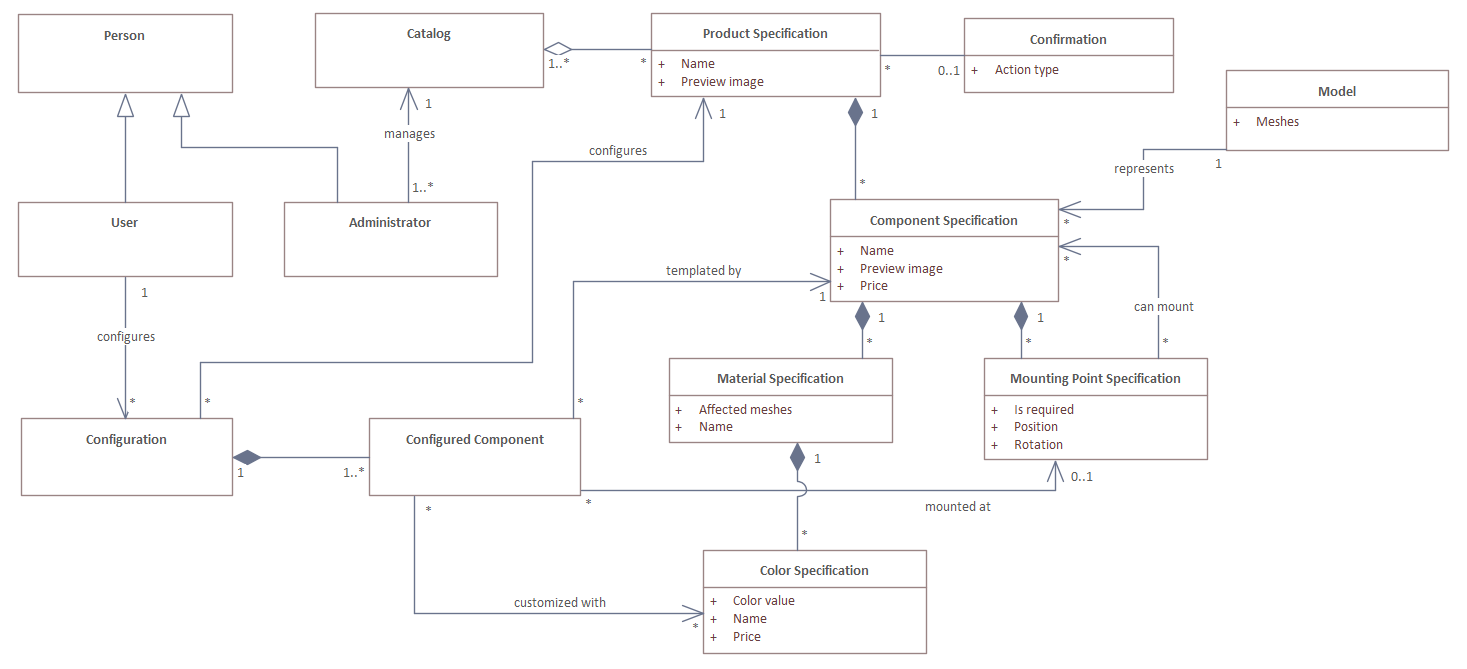
\includegraphics[width=\linewidth]{images/uml_domainmodel.png}
\caption{Domain model as a UML diagram}
\label{fig:domain-model}
\end{figure}
\end{landscape}

% - - - - - - - - - - - - - - - - - - - - - - - - - - - - - - -
\subsection{Catalog}
% - - - - - - - - - - - - - - - - - - - - - - - - - - - - - - -

The catalog forms the backbone of the proposed toolkit and defines the blueprint for customizable products. The catalog encompasses a variety of product specifications, each defining a configurable product along with all its potential customizations. This section delves into how these specifications lay the foundation for user-driven product configuration.
The entities discussed in this section are as follows:
\begin{itemize}[label=\rectanglebullet]
    \item Catalog
    \item Product Specification
    \item Component Specification
    \item Model
    \item Mounting Point Specification
    \item Material Specification
    \item Color Specification
    \item Administrator
\end{itemize}

A product specification acts as an overreaching comprehensive concept that encompasses all aspects of a given product. The entity may incorporate an action to finalize the configuration of the product, fulfilling the need for confirmation of the configuration (see requirement \hyperref[itm:F10]{F10}). Given that the tool focuses on the handling of modular products (see requirement \hyperref[itm:F3]{F3}), it is imperative that each product consists of various components. Therefore, the product specification is made up of component specifications, which represent all the various possible components that the product can have.

To meet the requirement of 3D visualization (see requirement \hyperref[itm:F3]{F3}), component specifications must be linked to a model featuring 3D meshes. This model acts as a representation of the component that will be presented to the user during the configuration process. In addition to this, the component specification is composed of material specifications and mounting point specifications.

Material specifications are needed with respect to the requirement of material color configuration (see requirement \hyperref[itm:F8]{F8}). They describe the materials of a given component that the user can customize, with each material specification providing mesh information specifying which part of the component this material influences, thereby enabling preview updates as the user makes selections. In addition, the material specification consists of color specifications that define the possible colors this material can take on in the configuration process.

Mounting point specifications are introduced to address the requirement of fixed point component placement (see requirement \hyperref[itm:F6]{F6}). They represent points on a component to which other modular components can be attached. The specifications of mounting point include the relative position and rotation of the point, the requirement for a component's presence at this point, and possible specifications of components that can be mounted on the point.

All these specifications are maintained in the catalog by the application administrator, who has the authority to modify any properties. The tool then utilizes these specifications to enable the configuration of tangible products.


% - - - - - - - - - - - - - - - - - - - - - - - - - - - - - - -
\subsection{Configuration}
% - - - - - - - - - - - - - - - - - - - - - - - - - - - - - - -

Transitioning from potential to actual, the configuration section delves into how users bring customizable products to life through the toolkit.
It illustrates how configured components are the building blocks of user-generated configurations, embodying the transformation from a generic template into a product uniquely tailored to individual preferences.
The entities covered in this section include:
\begin{itemize}[label=\rectanglebullet]
    \item Configuration
    \item Configured Component
    \item User
\end{itemize}

Users of the application create configurations. The cornerstone of a configuration lies in its configured components. The specifications described in the previous section serve as templates for these configured components. While the specifications outline all the configuration options, a configured component indicates a particular option selected by the user. Beyond the base component specification, a configured component also stores the mounting point to which it is attached, as well as the selected colors of its materials. Thus, a configuration is composed entirely of these individually configured components.


%______________________________________________________________
\section{User interface}
%---------------------------------------------------------------

The design of the user interface plays an essential part in the development of such a tool because it significantly influences user satisfaction when interacting with the tool. Good preparation of user interface design helps to determine the direction and streamline the implementation, as well as making clear from the beginning how to deal with factors such as responsiveness (see requirement \hyperref[itm:NF2]{NF2})

In this section, low-fidelity wireframes are used to depict the proposed user interface, highlighting the layout and architecture of the application. This approach captures the most important information at this stage, leaving the finer details to be refined as part of the implementation phase.

The design is based on the analysis of existing solutions and respects the design principles of similar solutions that are most intuitive and the users may already feel familiar with.

The configurator as an application is specific in that it primarily centers around the configuration process, with this interface being the most important and all other interfaces being secondary. In this section, the design of this configuration screen will be introduced, as well as the introductory and confirmation screens.

The common element of all screens is the top bar with the logo of the business that operates the configurator, which should redirect the user to the main website of the company when clicked. All of this should be customizable in the admin settings of the application.

% - - - - - - - - - - - - - - - - - - - - - - - - - - - - - - -
\subsection{Configuration screen}
% - - - - - - - - - - - - - - - - - - - - - - - - - - - - - - -

\begin{figure}[h]
\centering
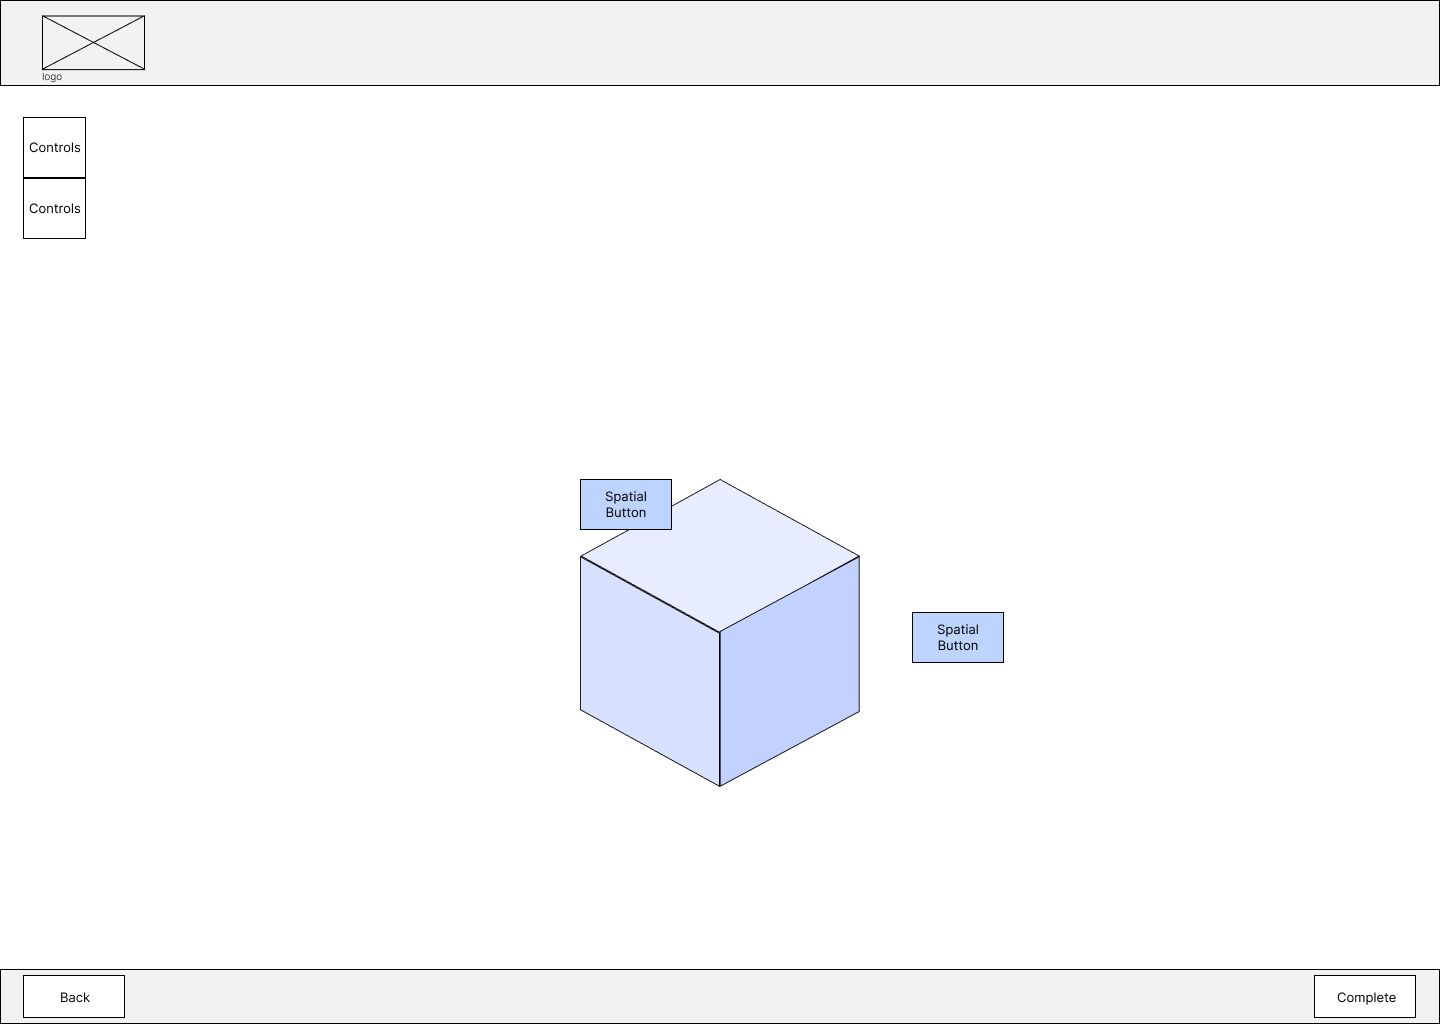
\includegraphics[width=0.7\textwidth]{images/wireframe_configuration_default.png}
\caption{Wireframe of configuration screen}
\label{fig:wireframe-configuration}
\end{figure}

The configuration screen is presented to the user during the configuration process. The screen is dominated by the 3D preview of the configured product, featuring interactable components and spatial buttons for the addition of components into the configuration. Control buttons are placed in the upper left corner within the 3D preview, symbolizing their direct relation to the preview, yet maintaining their distinctiveness as a separate element. At the bottom of the screen, there is another bar, this one containing buttons that allow users to go back or to finalize the configuration. The wireframe of the configuration screen in its default state is shown in  \autoref{fig:wireframe-configuration}, where the 3D preview of the product is represented by a blueish cube.

\begin{figure}[h]
\centering
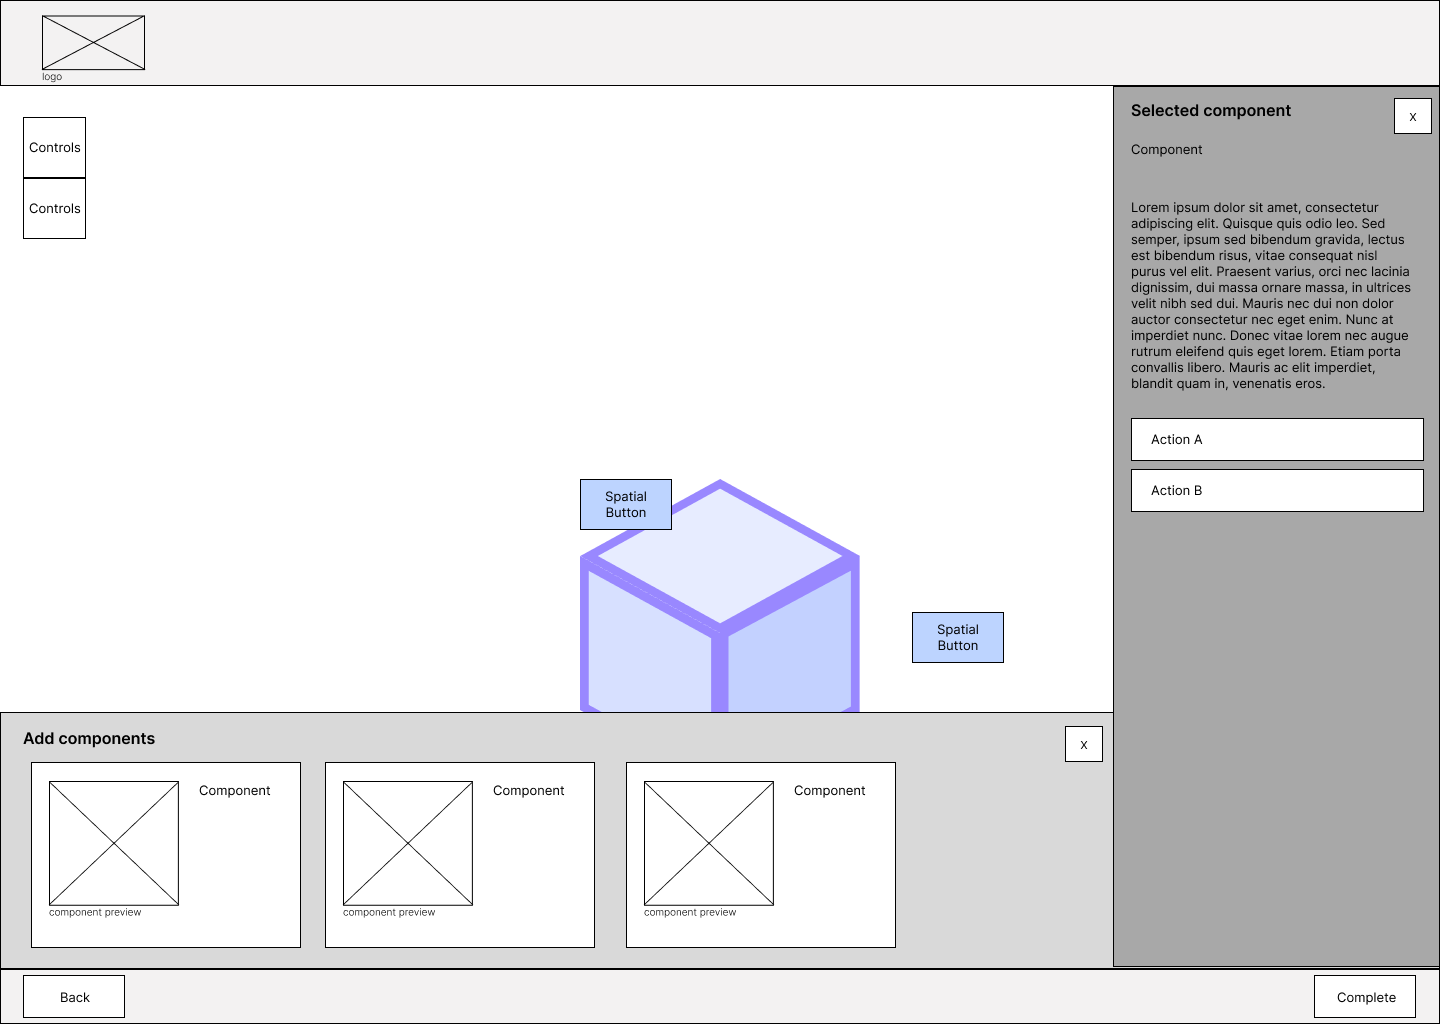
\includegraphics[width=0.7\textwidth]{images/wireframe_configuration_panels.png}
\caption{Wireframe of configuration screen with panels}
\label{fig:wireframe-configuration-panels}
\end{figure}

This default view, as outlined in the previous paragraph, maximizes the viewport with the most important presentation, which is the 3D preview of the product. However, at some stages of the configuration process, it is also necessary to present the user with further information. Therefore, upon selecting a component within the 3D preview, the component should become highlighted and, following the approach of existing solutions analyzed, a side panel with detailed information about the selected component will emerge from the right. If necessary, another panel with further options presented to the user may appear at the bottom. This design strategy maximizes the screen space for the important elements while still being flexible enough to present additional information in a streamlined way. The wireframe of the interface with panels that contain additional information and options presented is shown in \autoref{fig:wireframe-configuration-panels}.

\begin{figure}[h]
    \centering
    \begin{minipage}{0.4\textwidth}
        \centering
        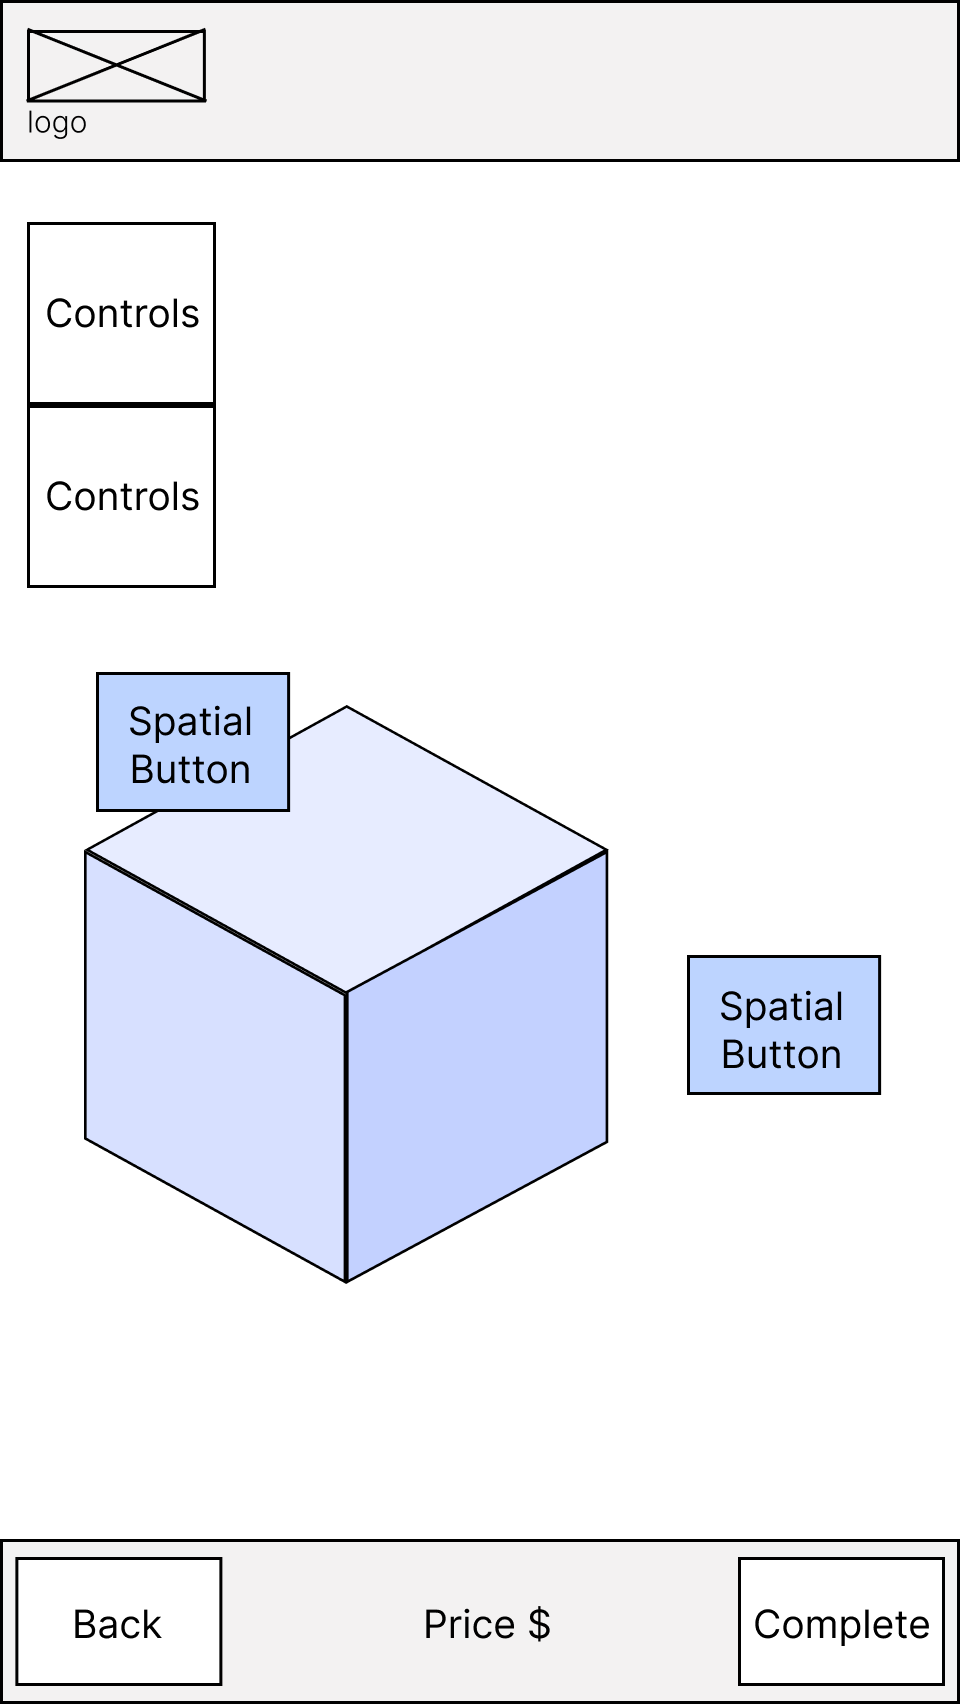
\includegraphics[width=\linewidth]{images/wireframe_configuration_mobile_default.png}
        \caption{Wireframe of mobile configuration screen}
        \label{fig:wireframe-configuration-mobile}
    \end{minipage}\hfill
    \begin{minipage}{0.4\textwidth}
        \centering
        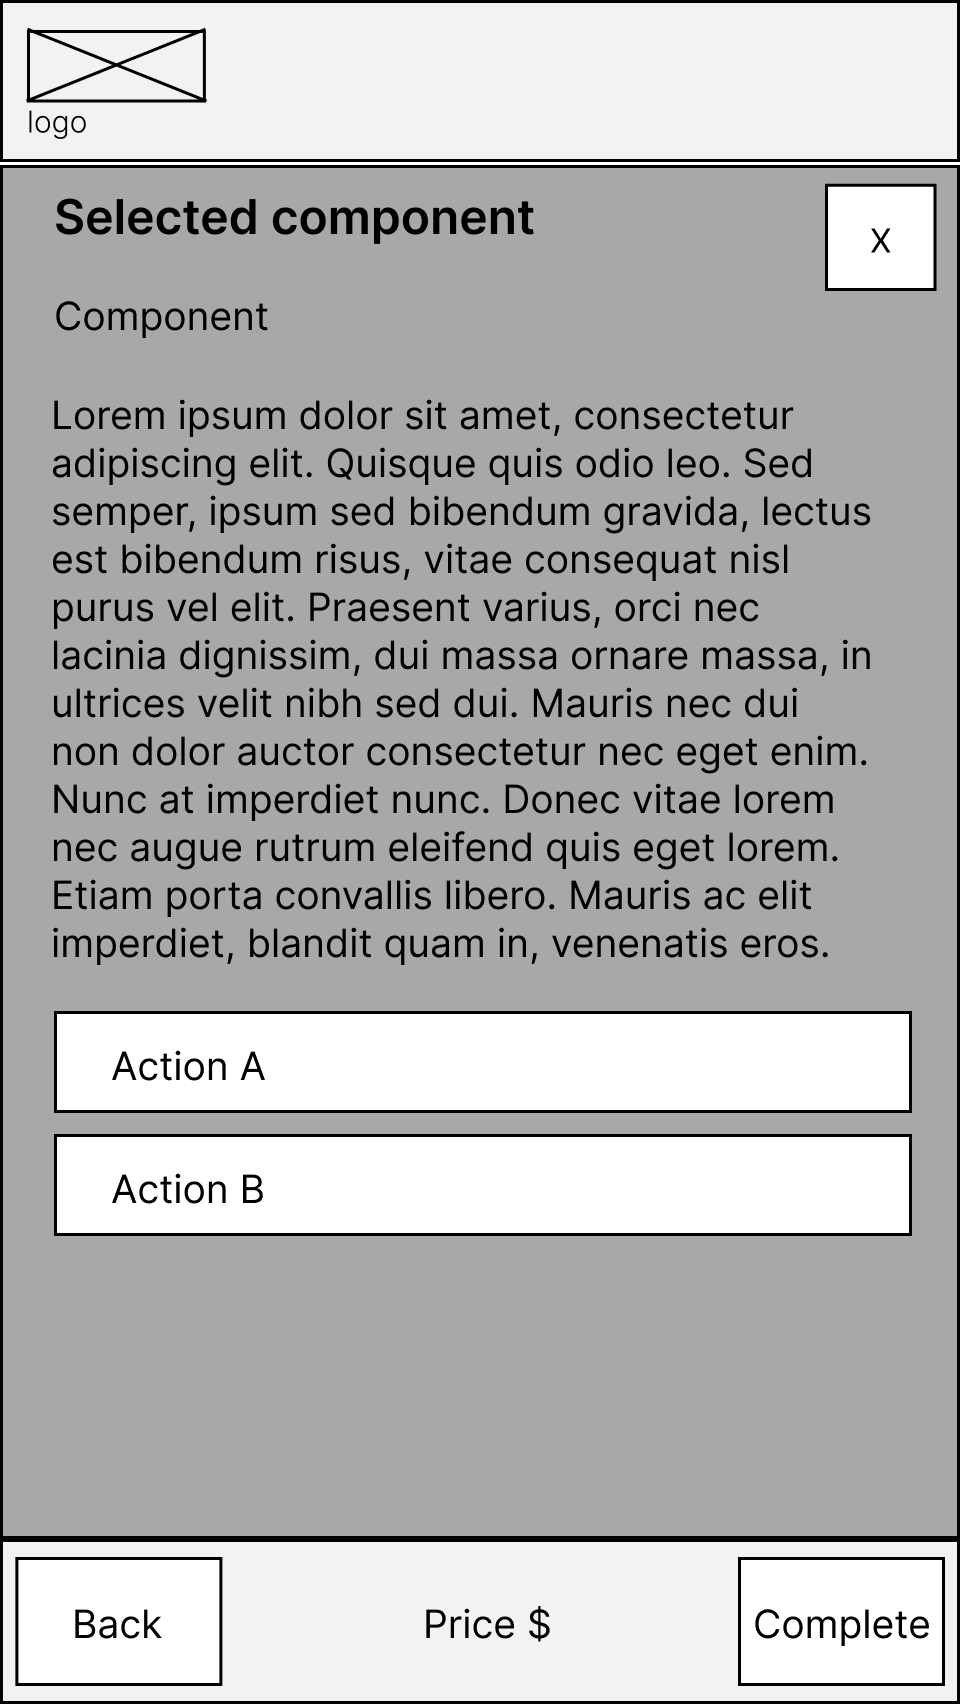
\includegraphics[width=\linewidth]{images/wireframe_configuration_mobile_panels.png}
        \caption{Wireframe of mobile configuration screen with panels}
        \label{fig:wireframe-configuration-panel-mobile}
    \end{minipage}
\end{figure}

To ensure responsiveness, a mobile version of the interface should also be outlined. The prioritization of the 3D preview in the default state makes this simple, as this just means that on smaller viewports the elements are presented in the same way, with the preview being in different aspect ratio, which is easily compensated by the 3D preview taking on different zoom level. The outline of this wireframe is presented in \autoref{fig:wireframe-configuration-mobile}.

The wireframe for the mobile version of the interface with the presented detail side panel is shown in \autoref{fig:wireframe-configuration-panel-mobile}. At this reduced viewport size, the side panel can maintain the same internal layout but to be usable it needs to occupy the whole 3D preview. This will need to be kept in mind when utilizing interactions with the 3D preview, as it may not always be fully visible when the panels are active. 

The design remains mostly consistent on both small and large viewports, while still being adaptive and responsive. This ensures that the familiarity with the tool is maintained for all viewport sizes.

% - - - - - - - - - - - - - - - - - - - - - - - - - - - - - - -
\subsection{Introduction screen}
% - - - - - - - - - - - - - - - - - - - - - - - - - - - - - - -

\begin{figure}[h]
\centering
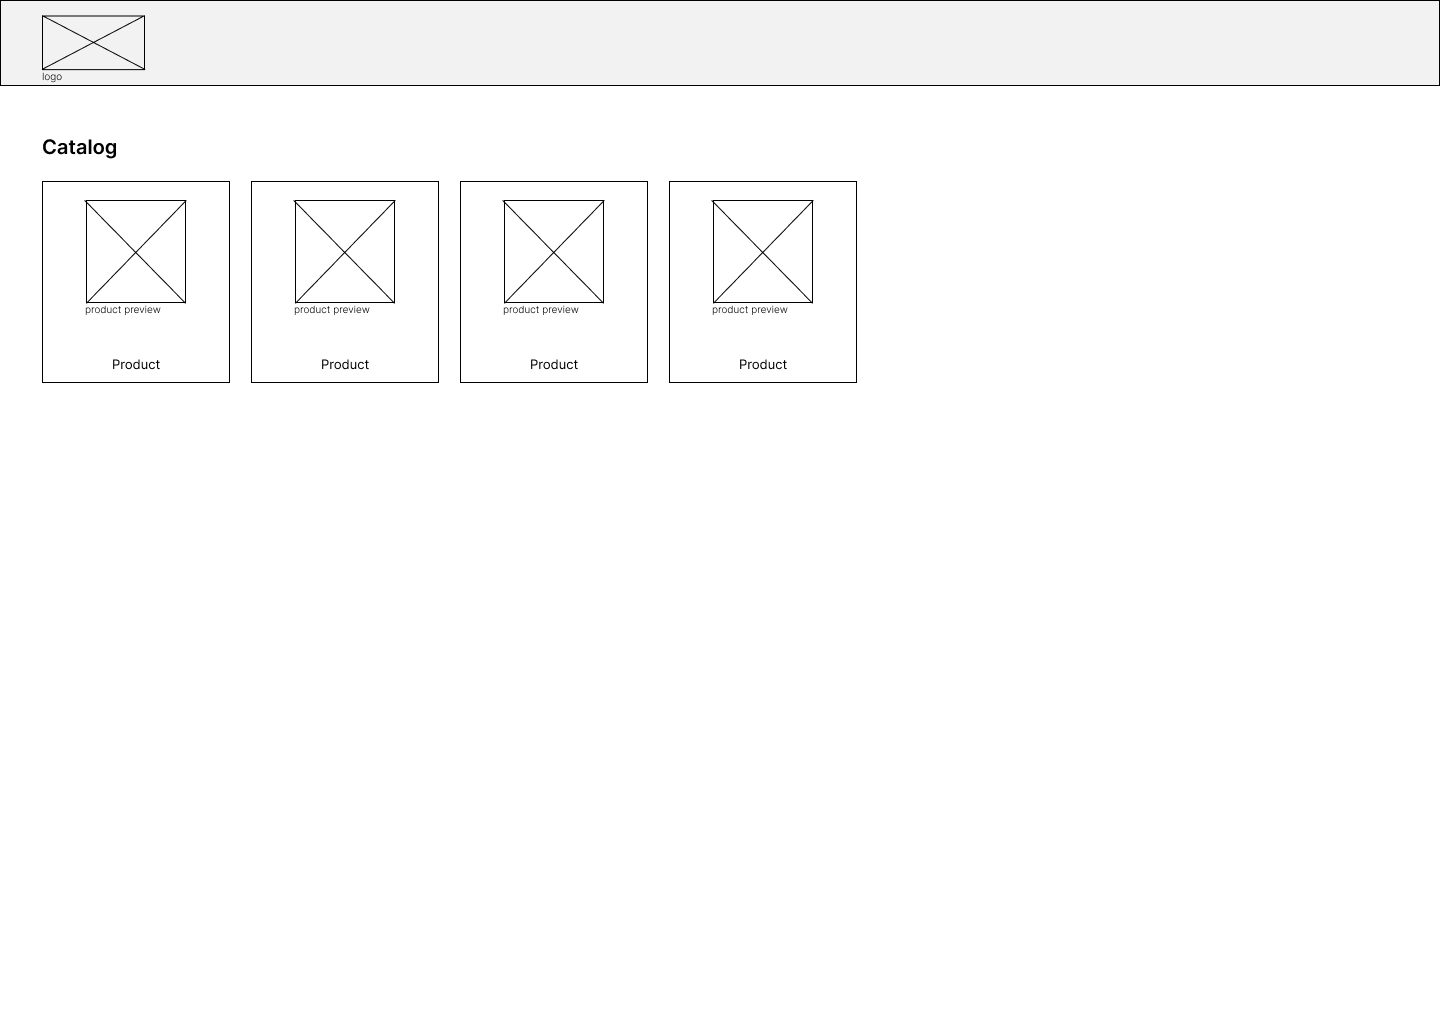
\includegraphics[width=0.7\textwidth]{images/wireframe_introduction_default.png}
\caption{Wireframe of introduction screen}
\label{fig:wireframe-introduction}
\end{figure}

The introduction screen is the first screen presented to the user when launching the application. It offers a simple way of selecting the configurable product from the catalog, with image and name of the product presented on a large tile. The selection of the product takes the user to the configuration process. Mobile interface of this screen mirrors the large version. The wireframe of the design can be seen in \autoref{fig:wireframe-introduction}.

% - - - - - - - - - - - - - - - - - - - - - - - - - - - - - - -
\subsection{Confirmation screen}
% - - - - - - - - - - - - - - - - - - - - - - - - - - - - - - -

\begin{figure}[hb]
\centering
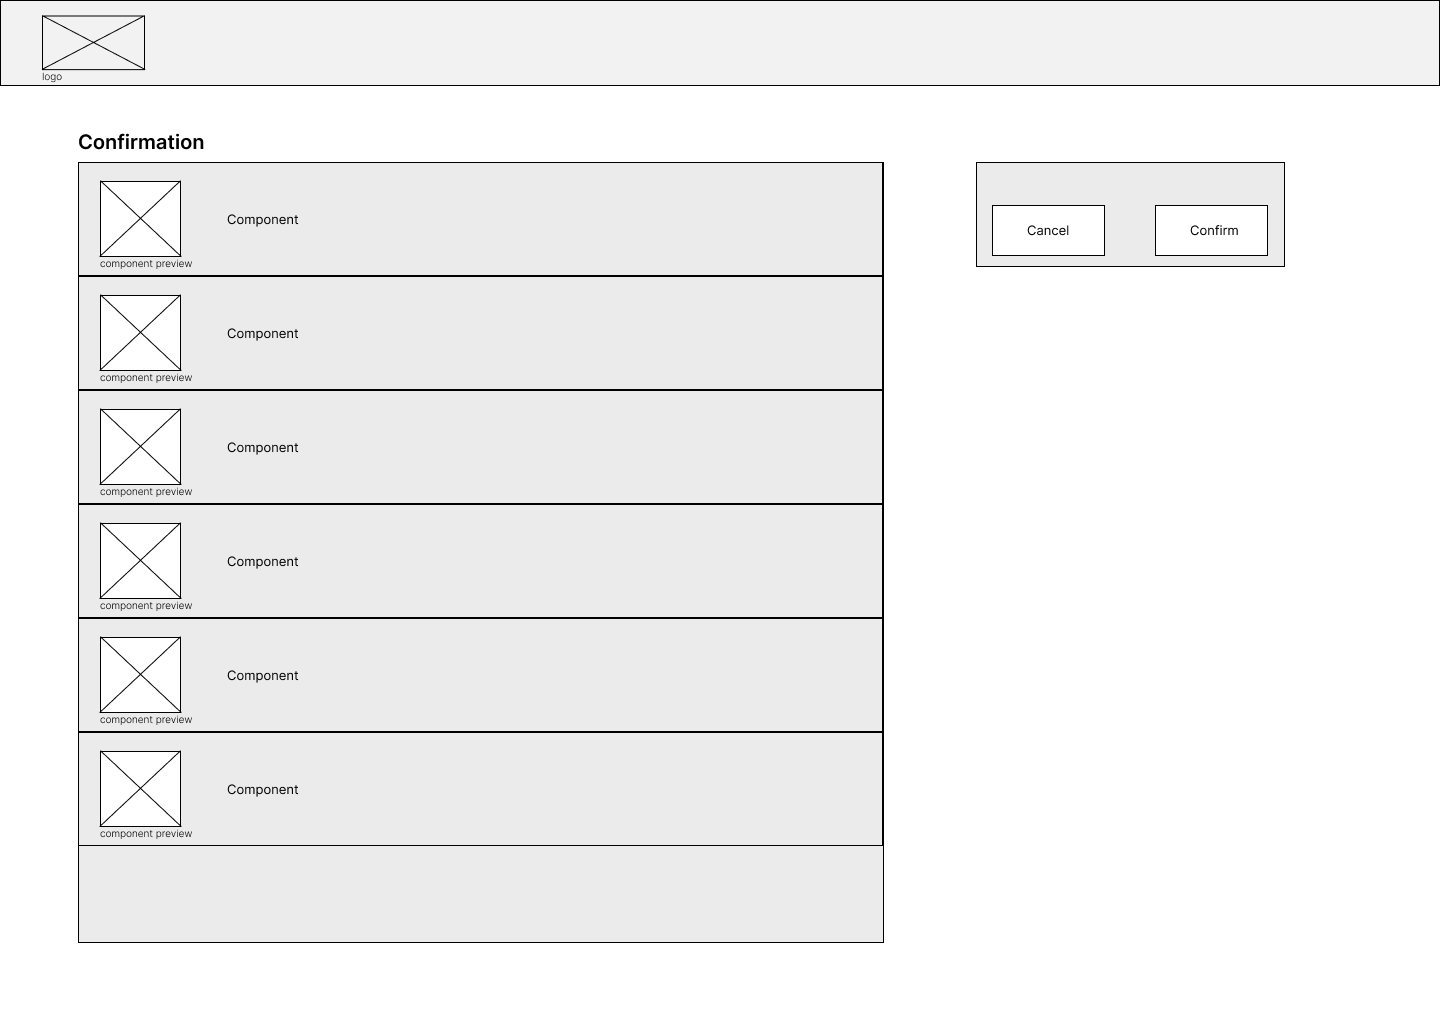
\includegraphics[width=0.7\textwidth]{images/wireframe_confirmation_default.png}
\caption{Wireframe of confirmation screen}
\label{fig:wireframe-confirmation}
\end{figure}

The confirmation screen is presented to the user at the end of the configuration and satisfies the configuration review requirement (see requirement \hyperref[itm:F9]{F9}). The wireframe of the configuration screen is shown in \autoref{fig:wireframe-confirmation}. On the left side, the confirmation screen presents the selected and configured components in a comprehensive list and allows the user to review their choices. The right side of the screen contains two buttons, one to confirm the configuration, which can initiate the confirmation action, and another to return to the configuration process for any adjustments. 

\begin{figure}[h]
\centering
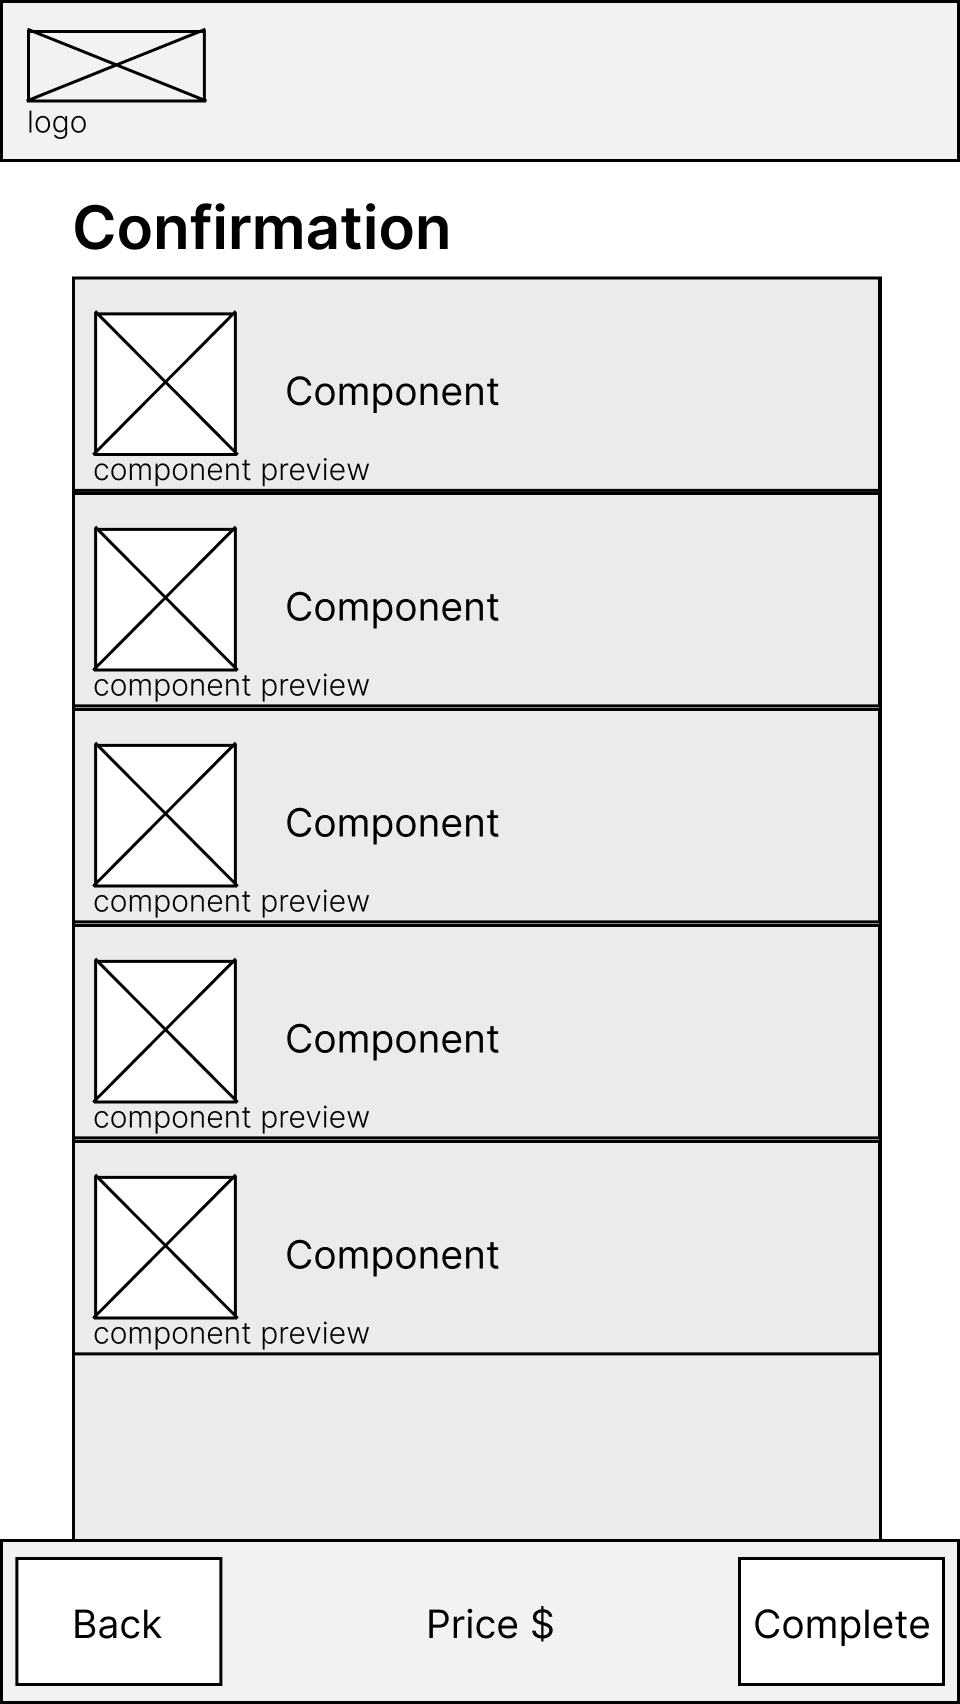
\includegraphics[width=0.3\textwidth]{images/wireframe_confirmation_mobile_default.png}
\caption{Wireframe of mobile confirmation screen}
\label{fig:wireframe-confirmation-mobile}
\end{figure}

The wireframe for the mobile version of the confirmation screen is depicted in  \autoref{fig:wireframe-confirmation-mobile}. In this layout, the summary spans the entire width of the screen, with the buttons moved to form a bar at the bottom of the screen.

\todo{Add prices to the wireframes and images and names to the domain model.}
\chapter{Implementation}

\begin{chapterabstract}
Lorem ipsum dolor sit amet...
\end{chapterabstract}

The following chapter will describe the implementation of the toolkit as envisioned in this thesis, building on the foundation created in the previous analysis and design chapters. 

Implementation focuses primarily on the requirements outlined in Chapter \ref{requirements}, with an emphasis on those of the highest priority. The output of this chapter is the realization of a viable and usable tool.

\section{Structure of the toolkit}

\section{Data schemas}

\section{Challenges and solutions}

\section{Views}
%\chapter{Deployment}

\begin{chapterabstract}
    Lorem ipsum dolor sit amet.
\end{chapterabstract}

In the following chapter, the attention is shifted from the development process to the deployment of the created solution. In this chapter, the focus is two-fold: firstly, the deployment of the solution is described in practical steps from the toolkit's administrator perspective, then business implications such as cost and process optimization are examined.

The setup of the solution is described from the point of view of a business wanting to utilize the tool. For illustration purposes, an example company is used in this chapter. The chosen company manufactures modular point-of-sale cardboard displays. To offer their product, they maintain a basic online presence using a simple website with information about the company and a showcase of their products, and a inquiry form which allows them to be contacted by their customer. In this scenario, the company aims to integrate the 3D configurator into its existing website to offer an interactive, user-friendly service that allows customers to customize and visualize options for their own configurations of cardboard displays.

By the end of this chapter, a comprehensive understanding of the deployment process of the toolkit from both a technical and business perspective will be provided.


%______________________________________________________________
\section{Application Setup and Configuration}
%______________________________________________________________

This section describes the necessary steps to utilize the implemented solution, from the perspective of a person designated by the business to operate the toolkit.


% - - - - - - - - - - - - - - - - - - - - - - - - - - - - - - -
\subsection{Building and Launching the Application}
% - - - - - - - - - - - - - - - - - - - - - - - - - - - - - - -

If the code of the application has been modified in any way, the installation of Node.js and npm is a prerequisite for building the application. The configurator application can then be built by executing \mintinline{bash}{npm install} followed by \mintinline{bash}{npm run build --workspace main}, which will generate the files in \texttt{apps/main/dist/} directory. If no modifications have been made, pre-built files may be utilized directly.

In the example case, the company already operates a website; therefore, the newly implemented configurator tool will be deployed to the appropriate subdomain of the website (e.g. \texttt{configurator.example.com}). This approach requires proper configuration of DNS settings for the new subdomain and appropriate adjustments to the web server, but otherwise utilizes the already existing web hosting infrastructure. If this were not the case, it would be necessary to facilitate an HTTP server through web hosting.

To deploy the application, the built files need to be copied to the web server, ensuring that they are statically served. The \texttt{index.html} file loads and initializes that application on access.

Due to the implementation of client-side routing, the web server needs to be adjusted to correctly redirect requests. A web server by default interprets request as a query for files located on the URL address, and since the routes defined in the application do not correspond to the actual files, the \textquote{not found} responses would be returned. Therefore, the server needs to be configured in such a way, that requests for nonexistent files are redirected to the \texttt{index.html} file, where they will be managed internally by React-Router. The company in the example case uses Apache HTTP Server, therefore its configuration \texttt{.httaccess} file, which sets the rules such that requests for nonexistent files, directories, or symlinks are redirected to \texttt{index.html} can be previewed in \autoref{listing:apache-config}. A similar setup can be achieved in comparable fashion with NGINX or other web servers.

\begin{listing}[h]
\begin{minted}{text}
RewriteEngine On
 
RewriteCond %{REQUEST_FILENAME} !-f
RewriteCond %{REQUEST_FILENAME} !-d
RewriteCond %{REQUEST_FILENAME} !-l
 
RewriteRule ^ index.html [L]
\end{minted}
\caption{Configuration of Apache HTTP Server client-side routing with React-Router}
\label{listing:apache-config}
\end{listing}

With this set, the application should be functional and available, albeit yet without the content of configurable products.


% - - - - - - - - - - - - - - - - - - - - - - - - - - - - - - -
\subsection{Customizing the Application}
% - - - - - - - - - - - - - - - - - - - - - - - - - - - - - - -

The following section describes the adaptation of the deployed application to meet the needs and correspond to the identity of the business. This is done by the administrator through modifications of the \texttt{appconfig.json} file.


\subsubsection{Localizations}

To adjust the interface texts and provide different localization options, translation files should be created in the \texttt{locales/} directory. This functionality is described in more detail in \autoref{section:impl-languages}. These translations can be based on the English translation file included with the built application. Once the necessary language files are set up (note that supporting English is optional), they should be listed by their two-letter codes in the \texttt{appconfig.json} file under the \texttt{ui.languages.all} key. Additionally, a default language must be specified in \texttt{ui.languages.default}.


\subsubsection{Appearance}

Following, the appearance of the interface can be tailored. Color scheme is customizable by updating the hex color codes in \texttt{ui.colors} and \texttt{spatialUi.selectionColors}. The logo displayed on the top left, as well as the favicon can be customized by setting the paths to the image files under \texttt{images} key. The web page to which the displayed logo links to can be configured using the \texttt{sources.homepageUrl} key. In addition, the title of the web page can be adjusted using the \texttt{title} key. The appearance customizations provide options for both dark and light modes of the interface.

Moreover, the camera style and floor shadow in the 3D visualization can be adjusted, and the option whether to display the button to save the completed configuration in PDF to users is provided.


\subsubsection{Data source}

Finally, the source from which the product catalog is fetched must be defined in \texttt{sources.catalogUrl}. Any accessible location which provides the files in the correct data scheme can be provided here. Creation of this catalog file is described in the following section.


\subsubsection{Example case}

In the example case discussed in this chapter, the interface was customized according to the company's brand guidelines. The company logo, set to appear in the top left corner, links back to the company's original website. The catalog source was defined as a static file located on the web server at \texttt{products/catalog.json}.


% - - - - - - - - - - - - - - - - - - - - - - - - - - - - - - -
\subsection{Catalog Creation and Content Management}
% - - - - - - - - - - - - - - - - - - - - - - - - - - - - - - -


The following section describes the process of managing configurable products for the deployed application.

The first step needed to create catalog of product is the preparation of 3D models that will be used in the configurator. The supported format is GLTF and its binary form GLB, to which other 3D formats can be converted. These files can be generated out of the CAD files used by the company to manufacture the products, or modeled manually. The images of the components that help the models with the representation should also be prepared and kept somewhere accessible.

It is necessary to store the files in an accessible location so that they can be fetched from their paths by the configurator application. It should be kept in mind that the size of the file and the complexity of the models correspond to the performance of the configurator application; therefore, it is beneficial to have simplified models with compressed textures to achieve the greatest possible performance. For easier of specification creation, the center of the model should also align with the center of the 3D scene in the file.

To create the configurable products, the administrative application needs to be launched. With the same prerequisites and dependencies as the main application, the admin tool can be built using the command \mintinline{bash}{npm run build --workspace admin}. The resulting files will be created in \texttt{apps/admin/dist}. These built files can be again uploaded to a web server (perhaps within the company intranet) or be served locally for the duration needed to create the specifications by executing \mintinline{bash}{npm run preview --workspace admin}.

Within the administrator's application Product Composer screen, product specification can be now created, by creating component specifications along with their materials, mounting points and specified base components. It should be kept in mind that the 3D models of the components (and images) in the admin application are loaded from the same paths as they will be in the main application during configuration, and it is therefore crucial for these models to be accessible in both applications on the same paths. When product specifications are created, they can each be exported to JSON files, and again, need to be stored in accessible locations from the main application.

The catalog is then created in the Catalog Composer screen of the admin application. Each catalog entry must reference the location accessible from the main application where the product specification file created in the previous step can be fetched from. After the catalog is complete, it should be exported and stored at the location specified in the global config file, which was discussed in previous section.

For updates of the created specifications, the existing files can be downloaded, updated, imported back into the admin tool, edited, and then uploaded back to their original locations.

In the example company followed in this chapter, the 3D models were generated from CAD software used in manufacturing process of the company and stored as static files on the web server. Then, the admin application was utilized to create the product specifications and catalog, The created files were also transferred to the web server, from where they will be statically served. Given that the company utilizes an inquiry form on their website, the configurable products followed the same approach and had an inquiry form set as a confirmation action. A serverless function, hosted on Cloudflare Workers\footnote{https://workers.cloudflare.com}, was created to process the data. The function accepts the POST requests with the contact info and configuration created by the user sent from the inquiry form within the main application, and forwards these data to a company email. To enable this, the URL of this serverless function was set as the endpoint of the confirmation action in the Catalog Composer screen. A simplified illustration of the implementation of serverless functions can be seen in \autoref{listing:serverless}.

\begin{listing}[h!]
\begin{minted}{typescript}
async function handleRequest(request: Request) {
  const headers = new Headers({
    "Access-Control-Allow-Origin": "configurator.example.com",
    "Access-Control-Allow-Methods": "POST, OPTIONS",
    "Access-Control-Allow-Headers": "Content-Type"
  });

  if (request.method === "OPTIONS") {
    return new Response(null,
        { headers, status: 204 });
  }
  if (request.method !== "POST") {
    return new Response("Method Not Allowed",
        { headers, status: 405 });
  }

  const formData = await request.json();
  try {
    const parsedData = RequestSchema.parse(formData);
    await sendEmail(parsedData);
    return new Response(null, 
        { headers, status: 200 });
  } catch (error) {
    return new Response("Invalid data",
        { headers, status: 400 });
  }
}

addEventListener("fetch", event => {
  event.respondWith(handleRequest(event.request));
});
\end{minted}
\caption{Implementation of serverless function for forwarding inquiry form data}
\label{listing:serverless}
\end{listing}


%______________________________________________________________
\section{Business Aspects}
%______________________________________________________________

This section explores the business aspects of deploying the configurator tool, examining the cost effectiveness as well as business process modifications within the company.


\subsection{Cost effectiveness}

As this solution aims to cater to small businesses, this project has been conceptualized with cost effectiveness in mind, with the requirement of lightweight infrastructure needs (\hyperref[itm:NF4]{NF4}) and self-hostability (\hyperref[itm:NF3]{NF3}). These principles have been greatly reflected in the design and implementation.

The primary costs of this solution stem from the setting up of the tool, which includes acquiring 3D models and specifying the configurable content, as well as the customization of the tool and integration into the infrastructure. These costs can vary greatly between different companies, as some may be disposing of the necessary files, while others will have to create them. The complexity of the offered products that are defined in the tool also plays a role in this step.

From a technical standpoint, the infrastructure costs are low. For companies with an existing web server, no additional infrastructure is required. In addition, the costs of web hosting are minimal, as static websites can often be hosted free on platforms such as Cloudflare Pages \cite{CloudflarePages} or Netlify \cite{Netlify}. 

For functionalities the require additional processing of the product data or the inquiry form, serverless functions, as demonstrated in the previous case, can be used. Unless a very large amount of requests is processed, these can also be very cost-effective, and the summary of the pricing per requests for three major serverless providers (Cloudflare Workers, AWS Lambda, Google Cloud Functions) as of April 2024 can be seen in \autoref{table:lambda-price}.

\begin{table}[htb]
\centering
\begin{tabular}{>{\raggedright\arraybackslash}p{4.1cm} >{\raggedright\arraybackslash}p{4cm} >{\centering\arraybackslash}p{3cm}}
\toprule
\textbf{Provider} & \textbf{Free plan limits} & \multrow{c}{\textbf{Cost over limit} \\ \textbf{(per million reqs)}}\\ 
\midrule
Cloudflare Workers & 100 000 reqs/day & \$0,15 \\
AWS Lambda & 1 000 000 reqs/month & \$0,20 \\
Google Cloud Functions & 2 000 000 reqs/month & \$0,40 \\
\bottomrule
\end{tabular}
\captionsource{Summary of the pricing per requests for serverless providers}{Cloudflare \cite{CloudflareWorkers}, Amazon \cite{AWS}, Google \cite{GoogleCloud}}
\label{table:lambda-price}
\end{table}


In the example company described in this chapter, the only expense associated with the tool was the time spent preparing the content and deploying the application.


\subsubsection{Return on Investment}

Consequently, the return on investment (ROI) for this solution is therefore projected to be hugely positive. While having minimal costs, the configurator not only acts as a sales assistance tool, allowing for detailed product visualization and customization, but also serves as a marketing tool that can enhance the company's market presence and appeal to a technically adequate consumer base. 


\subsection{Operational Impact}

To evaluate the impact deployment of the solution brings to businesses and companies is a complex task. The toolkit is adaptable and product-agnostic, meaning it can be utilized by different companies being in different fields or in different parts of a supply chain (such as reselling or manufacturing). Sequentially, the impact on processed will be different in each case.

This section will describe the change in processes after the tool deployment of the example company examined in this chapter, and should serve illustrate one of the effects this tool can have.  
%\chapter{Testing}

\begin{chapterabstract}
    Unit testing, system testing, usability testing and gained insights.
\end{chapterabstract}

Testing is an integral part of the software development process. This chapter provides an overview of the tests conducted during the development of this solution, as well as an evaluation and discussion of the testing results.

Software testing is essential for detecting malfunctions that may negatively affect the application's users and create further issues for the operator of the~software. Testing is also necessary to confirm that the solution complies with the set specifications and helps to validate the design choices made.~\cite{Homes2012}

There are various types of software tests, which can be categorized in many different ways, such as automated versus manual, functional versus non-functional, black-box versus white-box, by their coverage (unit versus whole system) or by their scope (performance versus compatibility). The choice of tests is always context-dependent and needs to be aligned with the project goals and limitations.~\cite{Krysik2023}

Testing 3D applications presents unique challenges that differentiate it from testing standard web applications, with main differences in user interactions. The developed solution enables users to move within a 3D space and interact with spatial objects. Interactions therefore occur in a 3D environment projected onto a 2D viewport, significantly expanding the range of possible interactions compared to traditional 2D applications. The potential interactions also vary depending on the product being configured in the application, as the solution aims to be product-agnostic, as well as further complicating matters with the~configurator's open navigation mechanism.

Unlike 2D applications where layout and style are the focus, 3D applications require tests to confirm that objects appear correctly from various angles and under different conditions. This aspect is challenging, as it is less straightforward than verifying the \noborderacrshort{dom} of a standard website, since in this scenario, the 3D preview is represented by a canvas element without a straightforward method for breakdown. In addition, loading 3D content is time and computationally consuming, which makes testing resource intensive. These complexities limit the applicability of certain types of tests, such as automated browser testing, which typically does not accommodate the nuances of working with 3D content.

Given these constraints and the goals of the solution, three distinct kinds of tests were performed during the development lifecycle of the application: unit tests, system tests, and usability tests. The tests performed are described in the following sections.


%______________________________________________________________
\section{Unit Testing}
%______________________________________________________________

Unit testing involves testing the smallest parts of the software, which are typically individual functions. The testing is performed in isolation from the~rest of the~system, with dependencies being mocked or stubbed to ensure that the tests are independent. These tests provide immediate feedback on the~functionality of the written code and help detect bugs or regressions when the~code undergoes changes during development. Since the resulting application is composed of these integrated parts, validating these parts helps with the~validation of the whole software.~\cite{Khorikov2020}

\begin{listing}[h!]
\begin{minted}{typescript}
describe("CatalogActions.getCatalog", () => {
  test(
    "returns the existing catalog " 
    + "if already present in the store",
    async () => {
      const existingCatalog = generateMock(CatalogSchema);
      storeMock.catalog = existingCatalog;

      const catalog = await CatalogActions.getCatalog(
        "http://example.com/catalog",
        storeMock);

      expect(fetchCatalog).not.toHaveBeenCalled();
      expect(catalog).toBe(existingCatalog);
    }
  );
});
\end{minted}
\caption{Example unit test used to validate store action within the solution}
\label{listing:unit-test}
\end{listing}

Due to the technologies chosen and the nature of the developed solution, the~majority of the~codebase is made up of code visualizing the products, written in markup language. This type of code is unsuitable for unit testing as it does not encompass any testable logic. However, parts of the solution that involve manipulation of data schemas in stores require complex logic and, therefore, these parts of the solution were subjected to unit testing.

The tests are stored in the \texttt{src/\_\_tests\_\_} directory. For the purpose of unit testing, the Jest framework\footnote{\url{https://jestjs.io}} was used, which enables a streamlined definition and execution of the tests. These tests can be run by executing the following command: \mintinline[bgcolor=backgroundgray]{bash}{npm run test}

Although tests should be isolated, they still operate with some data; therefore, these data schemas need to be mocked. Because data schemas were defined using the Zod framework (see \autoref{section:data-schemas}), the zod-mock\footnote{\url{https://www.npmjs.com/package/@anatine/zod-mock}} along with faker packages were used to quickly generate fake data from the schemas to be used in these tests, which closely resemble the values that will be used in real-world scenarios. An example of a defined unit test can be seen in \autoref{listing:unit-test}, which illustrates the generation of the mocked data, the calling of the tested function, and the verification of the results. Other unit tests are similar to the~one illustrated.

These tests validate the logic within the application and were run when committing changes to confirm the integrity of the updates made to the code during the development process.


%______________________________________________________________
\section{System Testing}
%______________________________________________________________

System testing verifies that all integrated components and subsystems of the~solution work as expected. This type of testing verifies that the application behaves as expected from the perspective of the user and that it meets the~specified requirements.~\cite{Stephens2023}

Due to the specifics of this solution outlined at the beginning of this chapter, this testing was not automated and was performed periodically manually during implementation. When defects were found, they were immediately addressed. Therefore, the evaluation of the fulfillment of the requirements, which should result from this testing, was done periodically and is described at the end of the implementation chapter (see \autoref{section:requirmenets-evaulation}).

To streamline this manual testing process, automatic deployment of the development environment was enabled using the GitLab \noborderacrshort{ci}/\noborderacrshort{cd} pipeline, which was triggered after each change to the codebase. To assess various different functionalities of the application, several different sample products, such as computer or shelves configurations, were created to enable the system testing process. 

To ensure the compatibility and responsiveness of the application across different browsers and operating systems, the LambdaTest platform\footnote{\url{https://www.lambdatest.com/}} was utilized. This platform enables the testing of web applications on thousands of combinations of major browsers and operating systems.~\cite{LambdaTest}

Therefore, the application was tested on a relevant sample of browsers. The~solution is designed to be compatible with all major browsers (Chrome, Firefox, Safari, Opera, Edge) with versions released from the year 2022 onward.


%______________________________________________________________
\section{Usability Testing}
%______________________________________________________________

Usability testing evaluates the functionality of the web application. In contrast with the system testing described in the previous section, usability tests employ real users. They are carried out by a facilitator, along with a selected sample of users, who perform tasks representative of actual usage situations. The~facilitator observes the users as they complete the tasks, noting their interactions with the system and their reactions. This allows to measure effectiveness, efficiency, and satisfaction of using the software. Usability testing is important, as it validates the proposed design from a fresh point of view, as the perception of the developed solution is different between the developer, who already knows every detail of the application, and the user, who has to learn how to work with the application.~\cite{Barnum2021}

Various categories of usability tests can be performed to assess different aspects of usability. Quantitative testing focuses on gathering numerical data about user experience, while qualitative testing collects observations and subjective feedback. In moderated testing, the user is led by the facilitator, compared to unmoderated testing, where the user is acting independently. Testing can be done remotely or in person, depending on available resources.~\cite{Moran2019}


% - - - - - - - - - - - - - - - - - - - - - - - - - - - - - - 
\subsection{Test Plan}
% - - - - - - - - - - - - - - - - - - - - - - - - - - - - - - 

Before the actual testing process takes place, it is necessary to establish what is tested, in what manner, who are the test participants, and how is the testing conducted and evaluated. The following section discusses these aspects of the~solution's usability testing.

In this thesis, usability testing is performed only on the configurator application. As discussed in the introduction of this thesis, the~enjoyment of the~configuration process itself directly influences the~perceived value of the~configured product~\cite{Franke2010}, therefore, it is imperative to ensure that the customer-centric configurator application is highly efficient and provides a great user experience in order to maximize the satisfaction of customers using the tool to configure their products.

Although usability testing could also be extended to the administrator part of the toolkit, it is important to note that the administrator application will be used only by administrators, which are only a few compared to the~users of the~configurator application. Administrators are also expected to have better technical knowledge than ordinary customers. The administrator part of the~toolkit is conceived to be used infrequently, typically during the~initial setup of the~tool or for occasional updates of the product catalog. Given these factors, the configurator part of the toolkit must comply with usability standards higher than those of the administrator part; therefore, the available testing resources are better allocated entirely to the configurator application.

Usability testing was performed in person and in locations that are natural to the participants, either at their workplaces or at their homes. Since the~solution requires no installation, the test participant's personal device was used to simulate real-world conditions and keep the participants comfortable.

The comfort of the test participant is important during the testing process, as anxious users can skew the results by not reacting the same way as they would naturally when using the tool outside of a testing context.~\cite{Nielsen1994}

Based on analysis of performed usability testing, research has revealed that, on average, five test participants are enough to reveal around 85\% of usability flaws, with additional participants providing diminishing returns in terms of unique feedback~\cite{Nielsen2000}. For this reason, the usability test was performed with five different users to efficiently gather as much comprehensive information as possible without overly intensive testing.  

During testing, standard approaches were followed. These include recording the sessions to enable for more objective processing afterward. The testing process was clearly explained, making it known to the~participant that the~solution is being tested, not the user, and therefore they are free to express themselves and will not be judged. In addition, the facilitator aimed to conduct the test in a way that does not lead or influence the test participant by helping in any way or asking suggestive questions during the testing process.~\cite{Moran2019}


%______________________________________________________________
\subsubsection{Evaluation Methods}

Usability testing was performed using both qualitative and quantitative methods.

To gather important context before the testing process, participants were, along with their general profile, asked about the following information: 
\begin{enumerate}
    \item Does the participant have any previous experience with online product configuration, has the participant ever used similar tool to preview or order a product?
    \item Does the participant have experience with 3D computer programs?
    \item When ordering custom products, does the participant prefer personal contact, such as phone or email communication, or would they rather use an~online configurator?
\end{enumerate}
This information is relevant, as the 3D controls employed in the developed solution are common; therefore, previous experience could impact the results of the usability test. In addition, the sentiment regarding the preferred shopping process could also influence the perceived usability of the tool.

During the process, the actions of the participants were observed and the~think-aloud method was used.

With the think-aloud protocol, participants are encouraged to reveal their thoughts during the process and to think out loud when using the application. This means that along with the actions taken, the information about why they have taken it is also immediately captured.~\cite{Moran2019}

After the test, a qualitative evaluation was done by conducting an interview with a general discussion about the solution, including the following questions:
\begin{enumerate}
    \item What difficulties did the participant encounter when using the tool? Was there anything particularly frustrating?
    \item What three improvements or features would the participant like to see?
    \item Did any part of the tool feel unnecessary or redundant?
    \item Is the product representation clear enough to understand what was configured?
    \item Would the participant use this tool in a real scenario to inquire configured products?
    \item What was the initial feeling of the participant about the tool?
\end{enumerate}

For quantitative evaluation, the \noborderacrfull{sus} questionnaire was used.

The \noborderacrshort{sus} is an industry standard for quickly evaluating the~usability of a~system. It consists of 10 questions, each with a numerical response on a scale from one to five, one representing \textquote{strongly disagree} and five being \textquote{strongly agree}. The questions are presented in \autoref{table:sus}.~\cite{Sus}

\begin{table}[htb]
\centering
\begin{tabular}{r>{\raggedright\arraybackslash}p{11.5cm}}
\toprule
1. & I think that I would like to use this system frequently \\
2. & I found the system unnecessarily complex \\
3. & I thought the system was easy to use \\
4. & I think that I would need the support of a technical person to be able to use this system \\
5. & I found the various functions in this system were well integrated \\
6. & I thought there was too much inconsistency in this system \\
7. & I would imagine that most people would learn to use this system very quickly \\
8. & I found the system very cumbersome to use \\
9. & I felt very confident using the system \\
10. &  I needed to learn a lot of things before I could get going with this system \\
\bottomrule
\end{tabular}
\captionsource{\glsentrylong{sus} questionnaire}{\cite{Sus}}
\label{table:sus}
\end{table}

A score is then calculated from the \noborderacrshort{sus} questionnaire as follows:
\begin{itemize}[label=\rectanglebullet]
    \item The response values for odd-numbered questions are subtracted by one.
    \item The response values for even-numbered questions are subtracted from five.
\end{itemize}
The adjusted responses are then added together and multiplied by 2.5, giving a~score between 0 and 100. This is calculated for each participant. To get a~single value that rates the~entire system, the average of these scores is taken.~\cite{Sauro2011}

Research of 500 usability studies has shown that the average \noborderacrshort{sus} score is 68. Therefore, a score above 68 suggests that the~solution is better than the~average system in terms of usability. However, it should be noted that this is a comparison with different types of systems, not necessarily with the same functionality. The 90th percentile is an \noborderacrshort{sus} score of about 80.3. \cite{Sauro2011}

The time to complete the tasks was not measured, as product configuration is a creative process where speed does not necessarily mean better performance. 


%______________________________________________________________
\subsubsection{Scenario}

For usability testing purposes, a mock product, a modular kitchen countertop, was prepared for configuration within the tool, with configurable components such as drawers, sinks, cabinets, corners and smooth edges.

Consequently, a single test case was used that involved the configuration of the defined kitchen product. This test case was broken down into several subtasks that participants were instructed to complete using the configurator application.

In the scenario presented to the users, the background context involved them renovating their homes and being in need of a new remodeled kitchen. They found a company specialized in custom kitchen furniture, which utilized a website where they used the developed solution to handle inquiries. The user has visited the configurator, at which point the usability testing has started. The subtasks were as follows:
\begin{enumerate}
    \item Create a configuration of kitchen modules in \textquote{L} shape. The left part of the~kitchen should include a drawer and sink, and the~right part of the~kitchen should contain two cabinets and another drawer.
    \item Add a smooth edges component to the edge modules.
    \item Set the color of the countertop of all the modules to \textquote{dark} and the wooden part of the modules to the color \textquote{cherry}. The color of the sink component should be set to \textquote{copper}, and the faucet to \textquote{gold} color.
    \item Review the created configuration and fill out and send an inquiry form with contact details.
\end{enumerate}

These product features and subtasks were selected to ensure that the~majority of functionalities of the~configurator application were tested by the~users in a single, comprehensive test case, which represented the~expected regular use. 


% - - - - - - - - - - - - - - - - - - - - - - - - - - - - - - 
\subsection{Testing Process}
% - - - - - - - - - - - - - - - - - - - - - - - - - - - - - - 

The following section describes the selection of participants for the usability test and provides a summary of the transcription from the testing process itself. 


%______________________________________________________________
\subsubsection{Participants}

As mentioned in the previous section, five participants were selected, which should be sufficient to uncover most usability issues. The participants were deliberately chosen to be heterogeneous, representing a range of different age groups, to ensure that the testing provided as much information as possible.

The participants, along with the contextual information gathered from them and the devices they used, are as follows:
\begin{enumerate}[label=\textbf{Participant \Alph*:}, leftmargin=*, itemindent=6.2em]
    \item \label{itm:A} 18 years old, male
        \begin{itemize}[noitemsep, label=\trianglebullet]
            \item \textbf{Experience:} Previous experience with 2D car configurator, also relevant experience with 3D modeling and extensive 3D gaming.
            \item \textbf{Device:} Desktop PC with Windows.
        \end{itemize}
        \vspace{4pt}
    \item \label{itm:B} 22 years old, female
        \begin{itemize}[noitemsep, label=\trianglebullet]
            \item \textbf{Experience:} Previous experience with 3D furniture configurator, also relevant experience with casual 3D gaming.
            \item \textbf{Device:} Mobile device with iOS.
        \end{itemize}
        \vspace{4pt}
    \item \label{itm:C} 46 years old, female
        \begin{itemize}[noitemsep, label=\trianglebullet]
            \item \textbf{Experience:} Previous experience with 3D furniture configurator, no other relevant experience.
            \item \textbf{Device:} Desktop PC with MacOS (with an Apple Magic Mouse).
        \end{itemize}
        \vspace{4pt}
    \item \label{itm:D} 52 years old, male
        \begin{itemize}[noitemsep, label=\trianglebullet]
            \item \textbf{Experience:} Previous experience with 3D car configurator, also relevant experience with 3D visualization software.
            \item \textbf{Device:} Laptop with MacOS (with a standard external mouse).
        \end{itemize}
        \newpage
    \item \label{itm:E} 62 years old, female
        \begin{itemize}[noitemsep, label=\trianglebullet]
            \item \textbf{Experience:} No previous experience with configurators or other relevant experiences.
            \item \textbf{Device:} Laptop with Windows (with a standard external mouse).
        \end{itemize}
\end{enumerate}
All participants expressed a positive sentiment towards using a configurator tool instead of a direct inquiry process.


%______________________________________________________________
\subsubsection{Execution and Observations}

The testing process began by preparing the tested application on the device and ensuring that there would be no interruptions during the testing.

The usability testing process, its purpose, and principles were then explained to the participants along with the three stages that it consists of: pre-test questions, the test itself, and post-test questions.

Questions were asked to establish context about the participant's background, experience, and sentiment, as detailed in the previous sections. The~responses can be found in the previous section along with other details about the participants.

The test of the application itself then began. The participants were reminded that it was the application being tested, not the user; therefore, they would not be judged and that any issues they may face are problems of the application's usability. Participants were also reminded that they would not be helped during the process but only observed, and were asked to think aloud and share their thoughts to help with this observation. The prepared scenario and the tasks they should complete were explained and presented to them on a sheet of paper for further easy reference. 

All participants immediately understood what to do and chose the initial component of the kitchen. The controls in the~3D space, along with the~buttons for the~addition of components, were also understood quickly by everyone. Therefore, the addition of the first components of the product was not problematic for anyone. 

However, as the configured product grew more complex, the addition of more components became an issue for everyone except Participant \hyperref[itm:A]{A}. The~problem was caused by an unclear scrolling pattern in the component addition menu. The menu pops up from the bottom of the screen, with horizontally laid tiles representing the mountable components. If there are more mountable components than would fit in this menu, horizontal scrolling is utilized. Due to the disappearance of the scroll bar and soft shading of the background, it was not clear to the participants that there could be more components accessible by scrolling horizontally. Although every participant has eventually figured it out, it has caused problems and frustrations, which, especially in the case of Participant \hyperref[itm:C]{C}, lasted several minutes. Furthermore, Participant \hyperref[itm:D]{D} has also suggested that a categorization of the available components on this panel would be beneficial for better orientation. 

Another observed pain point, which the majority of participants have also reported afterwards, was aggressive camera zooming. Whenever a component is selected, the camera tries to center the chosen component on screen. Almost all participants have reported that this movement is either too jarring and fast or that the zoom effect is too strong and that the 3D object should not be zoomed so much. 

\begin{wrapfigure}{r}{0.4\textwidth}
    \centering
    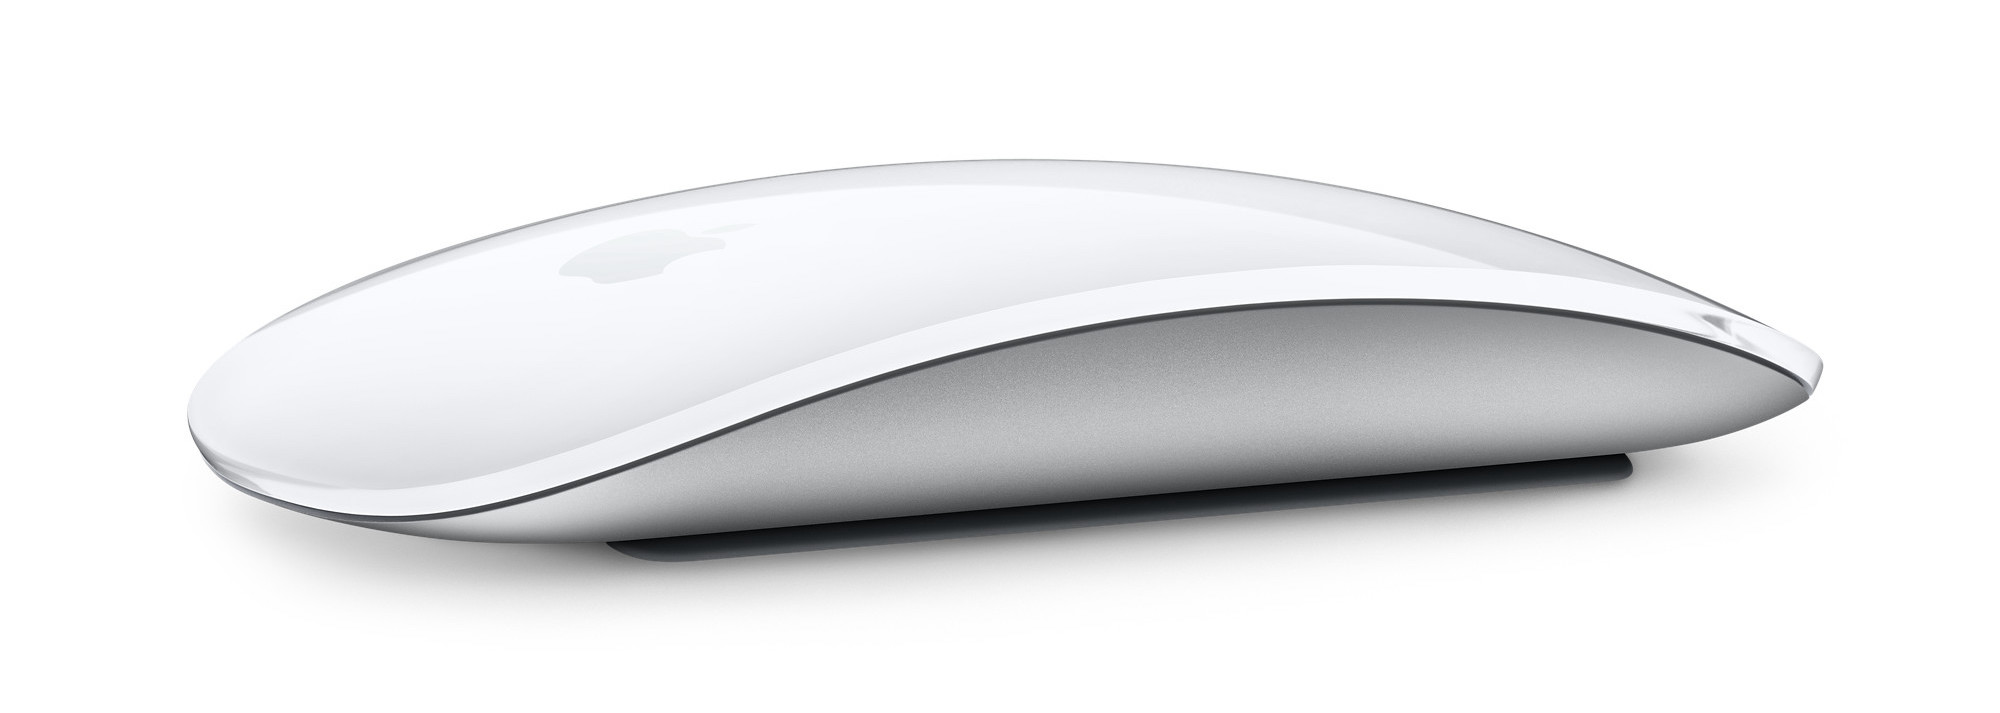
\includegraphics[width=0.35\textwidth]{images/image_magicmouse.jpg}
    \captionsource{Apple Magic Mouse}{Apple~\cite{MagicMouse}}
    \label{fig:magic-mouse}
\end{wrapfigure}

Participant \hyperref[itm:C]{C}, who used an Apple Magic Mouse with an unconventional button layout and gestures (see \autoref{fig:magic-mouse}), experienced particular difficulties. When trying to compensate for unwanted camera centering, the~participant accidentally performed a gesture on the mouse to navigate away from the application, restarting the whole configuration.

In addition to the selectable components in the 3D view, as a supporting element, there is also a small button symbolizing the component that also allows users to select it. This button is positioned at the~point where the~component is mounted. This has caused small issues for Participant \hyperref[itm:C]{C} and Participant \hyperref[itm:E]{E}. The post-test discussion revealed that the problem was caused by two things: the base component does not have a mounting point, therefore, the application does not have a button for this component, and at the same time the position of the button on the mounting point caused confusion as it was unclear to which component the button belongs to. The participants implied that it would be more intuitive if the button was placed in the center of the component.

Participants \hyperref[itm:C]{C} and \hyperref[itm:E]{E} also encountered small issues with the remove component button, which uses a hold-to-confirm mechanism instead of the traditional confirmation pop-up. The unfamiliarity with this mechanism has led both participants to require three attempts to perform this action. 

Participant \hyperref[itm:B]{B} expected that the review of components in the confirmation screen would be interactive, allowing for changes to the colors of the materials instead of merely reviewing them.

After overcoming these challenges, the participants quickly understood and completed the rest of the tasks without any further obvious problems. The~participants were then asked to complete the \noborderacrshort{sus} questionnaire on the~second side of the~instructions sheet, followed by an interview where the~previously detailed questions were asked.

In the post-test interview, a common wish among all participants except Participant \hyperref[itm:D]{D} was that the material color changes would apply to all components made of the same material, rather than having to adjust each one individually. Two participants also mentioned that the outline of the selected components was too wide and strong, obscuring the customized color. Participant \hyperref[itm:B]{B} has also expressed the desire to have the ability to change the environments in which the product is visualized.

Participants deemed no part of the tool redundant, except Participant \hyperref[itm:D]{D}, who considered the configuration review and confirmation screen unnecessary in the current form and suggested that a screenshot of the~3D preview of the~configuration should also be included there.

When asked about their initial feeling, three participants expressed that they wanted a guide or tutorial to be presented on the initial screen, and two participants mentioned that having preset configurations with prearranged components would be beneficial.  

All of the participants regarded the 3D product representation to be clear and understandable and all expressed that they would use this application in a~real scenario.


% - - - - - - - - - - - - - - - - - - - - - - - - - - - - - - 
\subsection{Test Results}
% - - - - - - - - - - - - - - - - - - - - - - - - - - - - - - 

The following section provides evaluation results and a summary of insights gained from the testing process, as detailed in the previous section.

The general sentiment regarding the usability of the tool was positive among all participants.

\begin{figure}[h!]
\centering
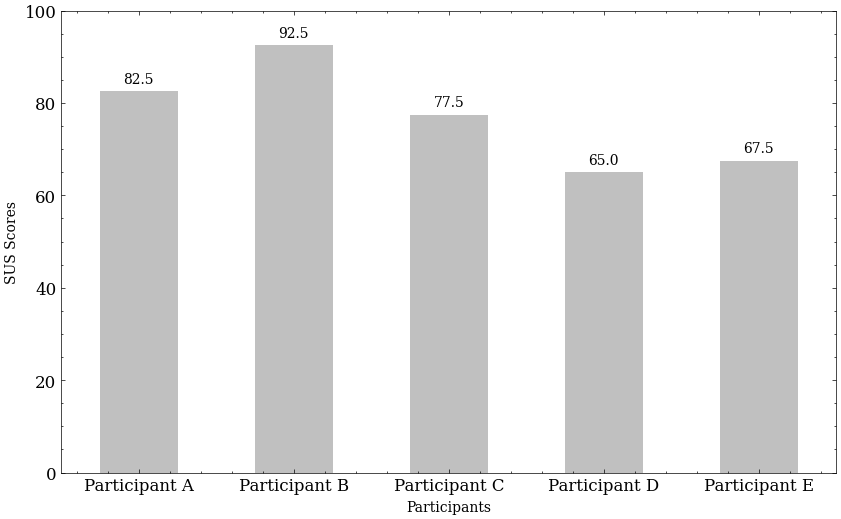
\includegraphics[width=0.95\textwidth]{images/graph_sus.png}
\caption{\glsentrylong{sus} scores by participant}
\label{fig:sus-scores}
\end{figure}


The average \noborderacrshort{sus} score for all participants was 77 which is considered good and above average when compared to other systems. The lowest \noborderacrshort{sus} score was 65, recorded by Participant \hyperref[itm:D]{D}, and the highest was 92.5, recorded by Participant \hyperref[itm:B]{B}. The scores for all participants are plotted on the chart shown in~\autoref{fig:sus-scores}.

A trend appears to indicate that the tool is more suitable for younger users. However, given the small sample size, this does not provide enough evidence to draw statistically significant conclusions in this regard.


%______________________________________________________________
\subsubsection{Insights} \label{section:insights}

The following section summarizes the issues identified during usability testing along with potential improvements, describes how fixes could be implemented, and reports the current status of these implementations. In addition, the~severity of each issue is estimated based on the difficulties observed during usability testing. The estimated severity was classified as high, medium, or low. The~priority for implementing fixes was based on the estimated severity.

\begin{enumerate}[label=\textbf{I\arabic*:}, leftmargin=27pt]
    \item Unclear scrolling pattern in component addition menu
        \vspace{2pt}
        \\Horizontal scrolling in the menu is not apparent (see \autoref{fig:screenshot-add-before}), leading users to believe that there are fewer available components than there really are.
        \begin{itemize}[noitemsep, label=\trianglebullet]
            \item \textbf{Severity:} High
            \item \textbf{Proposed fix:} Arrow buttons should be added as an additional apparent scrolling mechanism
            \item \textbf{Implemented:} Yes, see \autoref{fig:screenshot-add-after}
        \end{itemize}
        \vspace{2em}

        \begin{figure}[h]
        \centering
        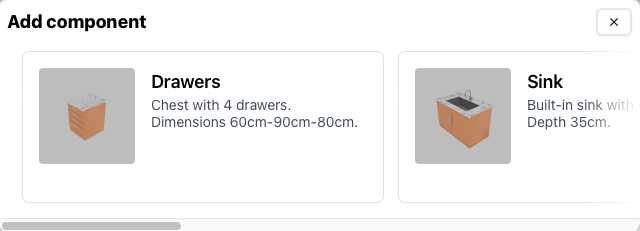
\includegraphics[width=0.7\linewidth]{images/screenshot_add-before.png}
        \caption{Component addition menu before the implemented fix}
        \label{fig:screenshot-add-before}
        \end{figure}
        \vspace{1em}
        \begin{figure}[h]
        \centering
        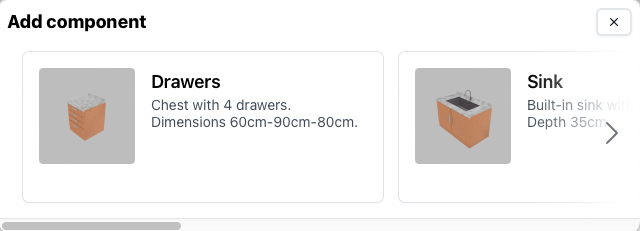
\includegraphics[width=0.7\linewidth]{images/screenshot_add-after.png}
        \caption{Component addition menu with implemented arrows for scrolling}
        \label{fig:screenshot-add-after}
        \end{figure}
    \newpage
    \item Jarring camera movement
        \vspace{2pt}
        \\The camera moves too abruptly and zooms in too much on component selection, causing discomfort and confusion among users.
        \begin{itemize}[noitemsep, label=\trianglebullet]
            \item \textbf{Severity:} High
            \item \textbf{Proposed fix:} The camera speed should be slowed down and limited to rotation only, avoiding zoom on component selection
            \item \textbf{Implemented:} Yes
        \end{itemize}
        \vspace{4pt}

    \item Incorrect position of the component selection button
        \vspace{2pt}
        \\The button supporting the selection of components is positioned at the~point the~component is mounted at, creating confusion about which component the button is associated with. The button is also missing on the base component.
        \begin{itemize}[noitemsep, label=\trianglebullet]
            \item \textbf{Severity:} Medium
            \item \textbf{Proposed fix:} The button representing the component should be centered within the 3D model and also added to the base component
            \item \textbf{Implemented:} Yes
        \end{itemize}
        \vspace{4pt}

    \item Excessive outline of the selected component
        \vspace{2pt}
        \\The outline of the selected component within the 3D preview can be too wide, obscuring the customized color of the component.
        \begin{itemize}[noitemsep, label=\trianglebullet]
            \item \textbf{Severity:} Medium
            \item \textbf{Proposed fix:} The width of the outline should be reduced or made transparent
            \item \textbf{Implemented:} Yes
        \end{itemize}
        \vspace{4pt}

    \item Lack of guidance
        \vspace{2pt}
        \\The tool does not provide users with any information about the controls.
        \begin{itemize}[noitemsep, label=\trianglebullet]
            \item \textbf{Severity:} Medium
            \item \textbf{Proposed fix:} A panel detailing the controls should be presented when first accessing the application and also be accessible by a button at any time
            \item \textbf{Implemented:} No
        \end{itemize}
        \vspace{4pt}

    \item Separated material changes
        \vspace{2pt}
        \\Changing the color of materials only affects a single component, even if there are other components with the same materials in the configuration. Therefore, updating the same material across all components requires \phantom{individually adjusting each one.}\newpage individually adjusting each one.
        \begin{itemize}[noitemsep, label=\trianglebullet]
            \item \textbf{Severity:} Medium
            \item \textbf{Proposed fix:} The data scheme for material specifications should be revised to not be part of the components but to be shared between them, alternatively, changing the color of a material could automatically update all components with the same material identification
            \item \textbf{Implemented:} No
        \end{itemize}
        \vspace{4pt}

    \item Missing preset configurations
        \vspace{2pt}
        \\The configurator does not provide users with precreated configurations on which the user could build upon.
        \begin{itemize}[noitemsep, label=\trianglebullet]
            \item \textbf{Severity:} Medium
            \item \textbf{Proposed fix:} Administrator should be able to create and offer product configurations which the user can use to derive their own configuration
            \item \textbf{Implemented:} No
        \end{itemize}
        \vspace{4pt}

    \item Unintuitive hold-to-confirm mechanism
        \vspace{2pt}
        \\The confirmation action used on the delete button, which requires holding the button for a while, is unintuitive.
        \begin{itemize}[noitemsep, label=\trianglebullet]
            \item \textbf{Severity:} Low
            \item \textbf{Proposed fix:} The hold-to-confirm mechanism should be replaced with standard confirmation popup
            \item \textbf{Implemented:} No
        \end{itemize}
        \vspace{4pt}

    \item Confirmation screen does not allow changes
        \vspace{2pt}
        \\The confirmation screen only offers an overview, and to make changes to the colors of materials, it is necessary to return to the configurator screen. In addition, the confirmation screen could provide more information.
        \begin{itemize}[noitemsep, label=\trianglebullet]
            \item \textbf{Severity:} Low
            \item \textbf{Proposed fix:} Changing colors of materials should be enabled directly from the confirmation screen, and the screen should present a screenshot of the preview of the 3D configuration
            \item \textbf{Implemented:} No
        \end{itemize}
        \vspace{4pt}

    \item Lack of categorization in the component addition menu
        \vspace{2pt}
        \\Categorization of components in the addition menu would improve user orientation and ease of use.
        \begin{itemize}[noitemsep, label=\trianglebullet]
            \item \textbf{Severity:} Low
            \item \textbf{Proposed fix:} A new category data scheme should be implemented to encompass different component specifications, and the menu should group the components based on their respective categories
            \item \textbf{Implemented:} No
        \end{itemize}
        \vspace{4pt}

    \item Blank environment in the 3D preview
        \vspace{2pt}
        \\The 3D preview features a blank background with color set by the~administrator, which can appear bland.
        \begin{itemize}[noitemsep, label=\trianglebullet]
            \item \textbf{Severity:} Low
            \item \textbf{Proposed fix:} Various 3D backgrounds should be introduced to allow visualization of the configured products in different environments
            \item \textbf{Implemented:} No
        \end{itemize}
        \vspace{4pt}
\end{enumerate}

Since only the most critical usability improvements were implemented, the remaining unimplemented usability enhancements could be the subject of further development of the tool and complement \autoref{section:improvements} on future improvements.

%\chapter{Conclusion}

The objective of this bachelor's thesis was to create an application for the 3D configuration of modular products.

To accomplish this goal, an analysis of existing solutions was performed, examining the perspective of both customers and the businesses operating such tools. Based on this, requirements for the solution implemented in this thesis were created, such that the created application provides businesses with an innovative solution for product configuration.

Consequently, a responsive web application was designed to support the configuration of a variety of modular products in a 3D environment. The configurator features open navigation, allowing users to customize modular products by adding or removing specified components at fixed points, and to customize their properties such as color of the materials. Additionally, advanced features such as collision detection were included to ensure that configurations are realistic and feasible. Further processing of the user-created configurations was made available by offering an integration using an API call to other systems or by presenting an inquiry form.

From a business perspective, the subsequent goals were for the  application to be flexible, lightweight, and easy to maintain, targeting smaller companies in need of a cost-effective solution. The developed tool is a front-end-only solution, set up by static files. To allow customers to configure their products, businesses can deploy the developed solution directly on their webservers. The tool as a whole has been separated into two separate applications: the user facing configurator and an administration tool allowing the business to define their configurable products.

In the design chapter, technologies were chosen and wireframes of the user interfaces were crafted.

The implementation chapter detailed the data schemas and the solutions to several interesting challenges encountered during implementation of the designed application.

In the deployment chapter, the deployment process was described within the context of a example business, highlighting the potential changes to business processes enabled by this solution.

Furthermore, the testing performed during the development of the application was discussed, including unit testing, system testing, and usability testing. Usability testing was conducted near the end of the development cycle to validate the functionality and user experience of the application, and the most severe usability issues were fixed.

Future improvements to this solution could include the creation of an accompanying back-end solution, integrations with existing e-Commerce platforms, or the implementation of a configuration rule evaluation engine. Possible future development directions are discussed in detail in \autoref{section:improvements}, and insights for user experience improvements from usability testing are also provided in \autoref{section:insights}.

The developed solution is freely available for businesses to use, enabling them to introduce modular product configuration on their websites effectively.

% Do not forget to include Introduction
%---------------------------------------------------------------
% \chapter{Introduction}
% uncomment the following line to create an unnumbered chapter
\chapter*{Introduction}\addcontentsline{toc}{chapter}{Introduction}\markboth{Introduction}{Introduction}
%---------------------------------------------------------------
\setcounter{page}{1}

% The following environment can be used as a mini-introduction for a chapter. Use that anyway it pleases you (or comment it out). It can contain, for instance, a summary of the chapter. Or, there can be a quotation.
\begin{chapterabstract}
	Product configurators and their value.
\end{chapterabstract}

Over the past few decades, the rise of e-commerce has caused a shift in consumer expectations, resulting in an increased demand for customized products. This gives rise to the need to shift focus towards mass customization, where products are customized according to individual preferences. To thrive in this sector, companies must modify their product offerings to be able to meet the unique needs of users. This necessitates the existence of a system (a toolkit), that enables customers to express their preferences and convert them into product configurations. \cite{Fulkerson2000}

The introduction of customization has been shown to significantly improve the customer's perception of the product's value. The involvement of consumers in the customization process leads to a stronger bond with the product, resulting in a perception of higher value compared to standard off-the-shelf products. This aspect of mass customization makes it an appealing and compelling strategy for businesses to implement. \cite{Schreier2006} However, when implementing such a system, it is crucial to ensure that the customization process is pleasurable for the customer. Research has shown that the enjoyment experienced during the customization also affects the perceived value of the final product, highlighting the importance of good implementation. \cite{Franke2010}

The task of transforming user preferences into concrete designs is a difficult endeavor that can be further hindered by a lack of effective communication between the customer's explanation of their desires and the business's comprehension. The use of online product configurators seemingly provides a solution for this issue by offering a user-friendly and visually appealing platform, which allows customers to customize products to their specifications, improves customer experience by increasing engagement and interactivity, and helps to bridge the gap between customer expectations and the end product. These tools have become an integral part of successful personalization strategies. \cite{Franke2003}

The introduction of modern technologies such as WebGL or Augmented Reality (AR) has expanded the potential of online configurators. These advances enable these toolkits to become more powerful and visually illustrative tools that provide a higher level of interactivity and realism than what was previously accessible. \cite{Cozzi2015}

%---------------------------------------------------------------
\section{Objective of this thesis}
%---------------------------------------------------------------

The primary objective of this thesis is to design and implement an application (toolkit) for the online configuration of modular products. The toolkit aims to be product-agnostic, adaptable, and customizable, usable by a variety of businesses, enabling their customers to interactively customize their modular products. The focus is on ensuring that the toolkit is not only flexible in accommodating various specific needs, but also straightforward for businesses to maintain after deploying, emphasizing lightweight infrastructure requirements. 
To accomplish this main objective, this requires an analysis of the characteristics found in current product configurators, as well as an examination of comparable solutions currently available to businesses.

%---------------------------------------------------------------
\section{Structure of this thesis}
%---------------------------------------------------------------

This thesis is divided into six chapters.

\begin{description}
\item[Chapter 1] The initial chapter entails an examination of existing solutions and an investigation into the functionalities that should be incorporated into this particular application.

\item[Chapter 2] The second chapter discusses the design of the application, the technologies chosen, the architecture, and the data structures.

\item[Chapter 3] The third chapter is devoted to implementation.

\item[Chapter 4] Chapter four focuses on the deployment of the implemented application in a particular business as an example. In addition, it discusses the resulting changes in the business processes of the selected business.

\item[Chapter 5] In the fifth chapter, the tests used in the development of the application are described.

\item[Chapter 6] Finally, the last chapter summarizes the results achieved and suggests possible directions for future development.
\end{description}


%---------------------------------------------------------------
\chapter{Analysis}
%---------------------------------------------------------------

\begin{chapterabstract}
	Lorem ipsum dolor sit amet. 
\end{chapterabstract}

Product configurators can be implemented in various ways, and the design of the tool itself determines the types of products that can be designed using the tool later on. The number of different unique configurations of a product that the tool can create is called the solution space. The size of the solution space is determined by two factors: the number of customizable attributes and the achievable values of each attribute. \cite{Huiwen2018} A relevant study examines the solution spaces of these toolkits and proposes an evaluation model that enables the categorization and assessment of various implementation approaches. Based on the target outcome and the guidance provided by the tool, the following mechanisms are specified: \cite{Hermans2012}

\begin{definition}[Veneer]
Customization by adding a visual decorative layer. (e.g. printing, engraving, etching)
\end{definition}
\begin{definition}[Modularity]
Customization by combining modules or components.
\end{definition}
\begin{definition}[Parametric]
Customization by changing the parameter values of parts.
\end{definition}
\begin{definition}[Generative]
Customization using code and scripting to synthesize the final form of the product.
\end{definition}

The main focus of this thesis is toolkits that primarily employ modularity mechanisms, however, there are often some common characteristics among configuration tools with different mechanisms.

\section{Exploring existing solutions}
\subsection{Configurators in use}

Currently, many companies are integrating product configurators into their sales strategies across multiple industries such as automotive, fashion, furniture, housing, and others. These configurators serve as either the main or supplementary sales tools for these businesses.

The Configurator Database Project by cyLEDGE MEDIA aims to catalog these web-based configuration tools. In the 2017/2018 report, they tracked 1250 deployments of these tools; however, the true count will be significantly higher since the database only includes the most frequently visited applications. \cite{cyLEDGE2018}

An analysis of the 100 most viewed configurators from May 2020 to May 2021 in the Configurator Database Project was performed in a study that examined the shared characteristics of these configurations. The results of some of the relevant characteristics and design choices that the study has analyzed are presented in this section: \cite{Blazek2023}
\begin{itemize}
    \item \textbf{Responsive design}: 75.3\% of examined tools had responsive design (the design adapted to the viewport of the device) 
    \item \textbf{Navigation}: 17.5\% of configurators had linear predefined navigation (meaning the configuration had to follow a specified sequence), whereas the majority of tools (82.5\%) had open navigation (user has the flexibility to configure the product in any order)
    \item \textbf{Visualization} 79.4\% of tools utilized photorealistic visualization (as opposed to illustrations or no visualization), however, the study acknowledges that there were significant variations based on the industries in which the configurator is utilized
    \item \textbf{Data transfer} The mean network data size transferred for 3D configurator was 35.6~MB
    \item \textbf{Configuration options} 60.8\% of configurators offered more than ten customizable attributes
    \item \textbf{Purchase capability} Given that car brands typically do not directly sell their cars online, it is logical to exclude them from the analysis of this particular characteristic. With the exclusion of vehicle configurators, 70.5\% of the configurators could complete an online purchase of the configured product
    \item \textbf{Price calculation} 56.7\% of the configurators were able to instantly reflect the changes made to the configuration in the displayed price
\end{itemize}

Another article also used the same database of configurators to analyze common design elements. They identified several key designs that were prevalent in the majority of configurators analyzed. The following key insights of common, recommended designs from the article are relevant to this thesis: \cite{Leitner2014}
\begin{itemize}
    \item At the end of the configuration process, a summary of selected options is presented
    \item To present the products that can be configured, images that are large enough to see details are used
    \item If the configurator has linear predefined navigation, the navigation information is presented on a horizontal plane
    \item Navigation bar is visible
    \item Price and order button is clearly visible and available for completion purposes
    \item Prices of the components are accessible in all phases of the configuration
    \item Logo is displayed prominently
    \item User preferences should be adaptable
\end{itemize}

As part of the analysis chapter of this thesis, it is essential to examine actual 3D~configurator applications. Due to the large number of existing applications, it is not within the scope of this work to perform an exhaustive analysis. Instead, this section will focus on a select group of four applications. These have been selected based on a combination of factors such as their popularity, functionality, and importance in the context of a modular product configuration. This selection is intended to provide insightful examples that highlight different approaches, rather than being representative of the entire domain.

\subsubsection{IKEA PAX planner tool}
\subsubsection{Lundia Original kastconfigurator}
\subsubsection{Muuto planner}
\subsubsection{LD Seating Nido}

\subsection{Offered toolkits}

\subsubsection{ThreeKit}
\subsubsection{Emersyea}
\subsubsection{Roomle} % include `text.tex' from `text/' subdirectory

\appendix\appendixinit % do not remove these two commands

\chapter{Additional visuals}

\begin{figure}
\centering
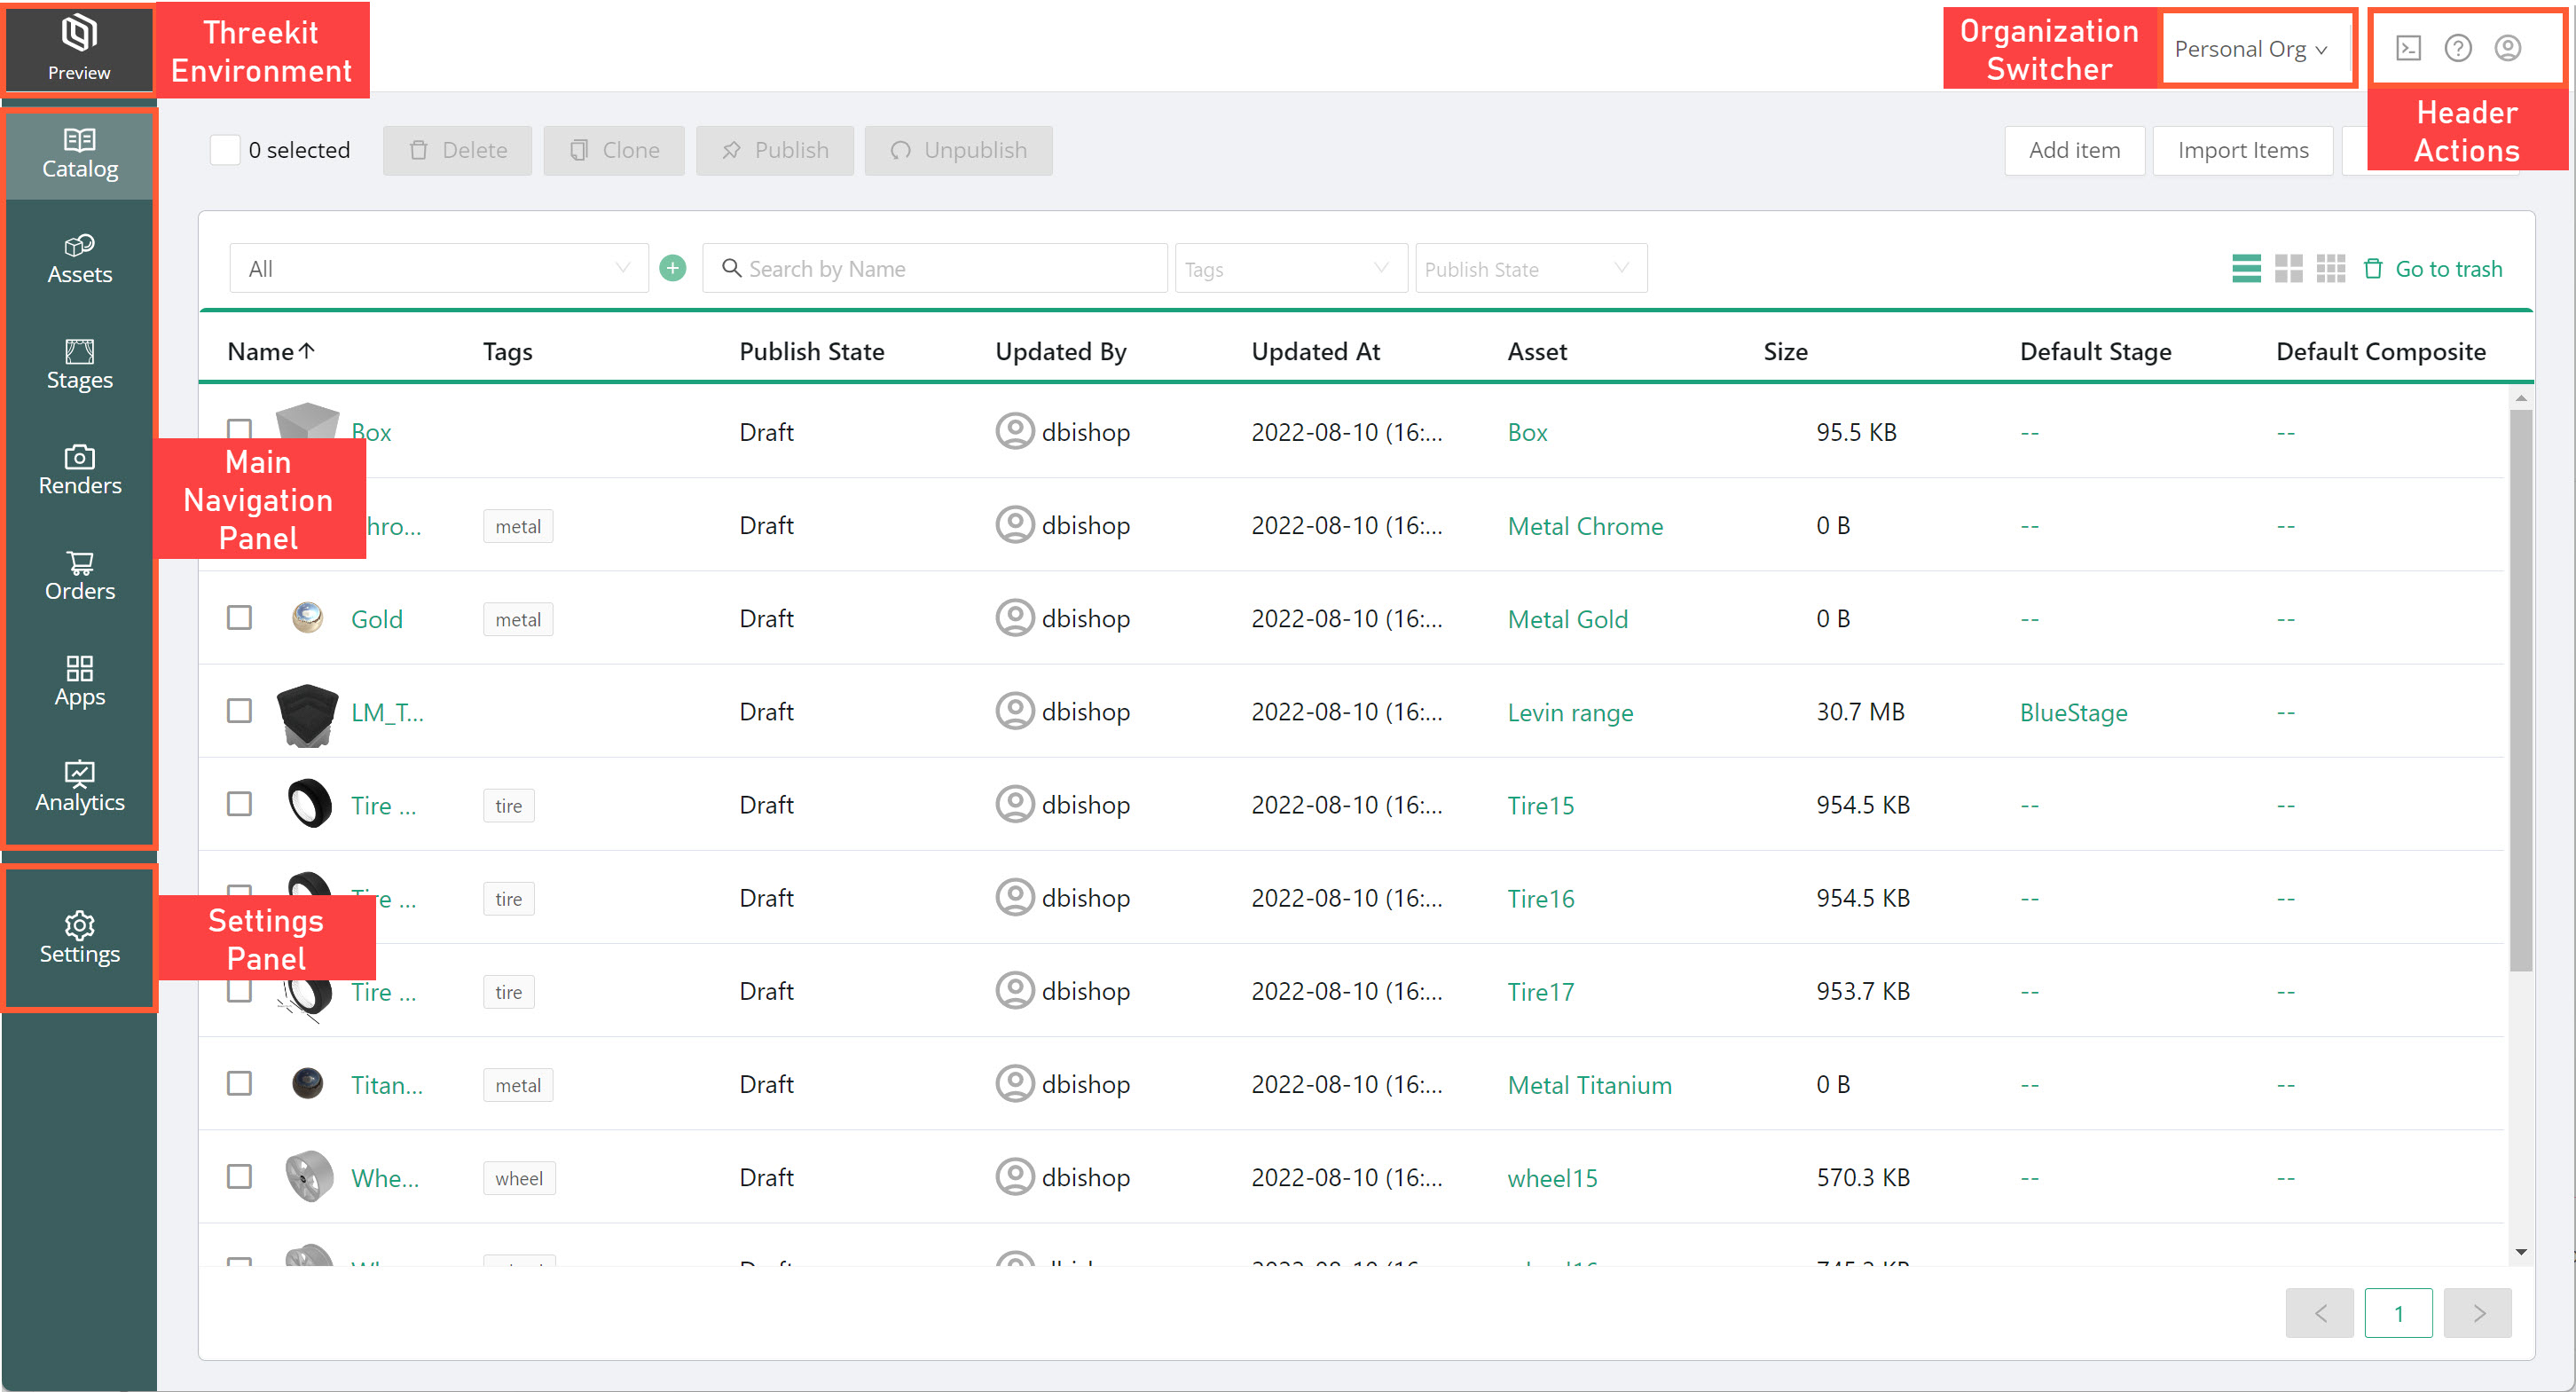
\includegraphics[width=14cm]{images/analysis_threekit-platform.jpg}
\captionsource{Threekit's Platform's landing page}{Threekit Platform Documentation \cite{ThreeKitPlatformDocumentation}}
\label{fig:threekit-platform}
\end{figure}

\begin{figure}
\centering
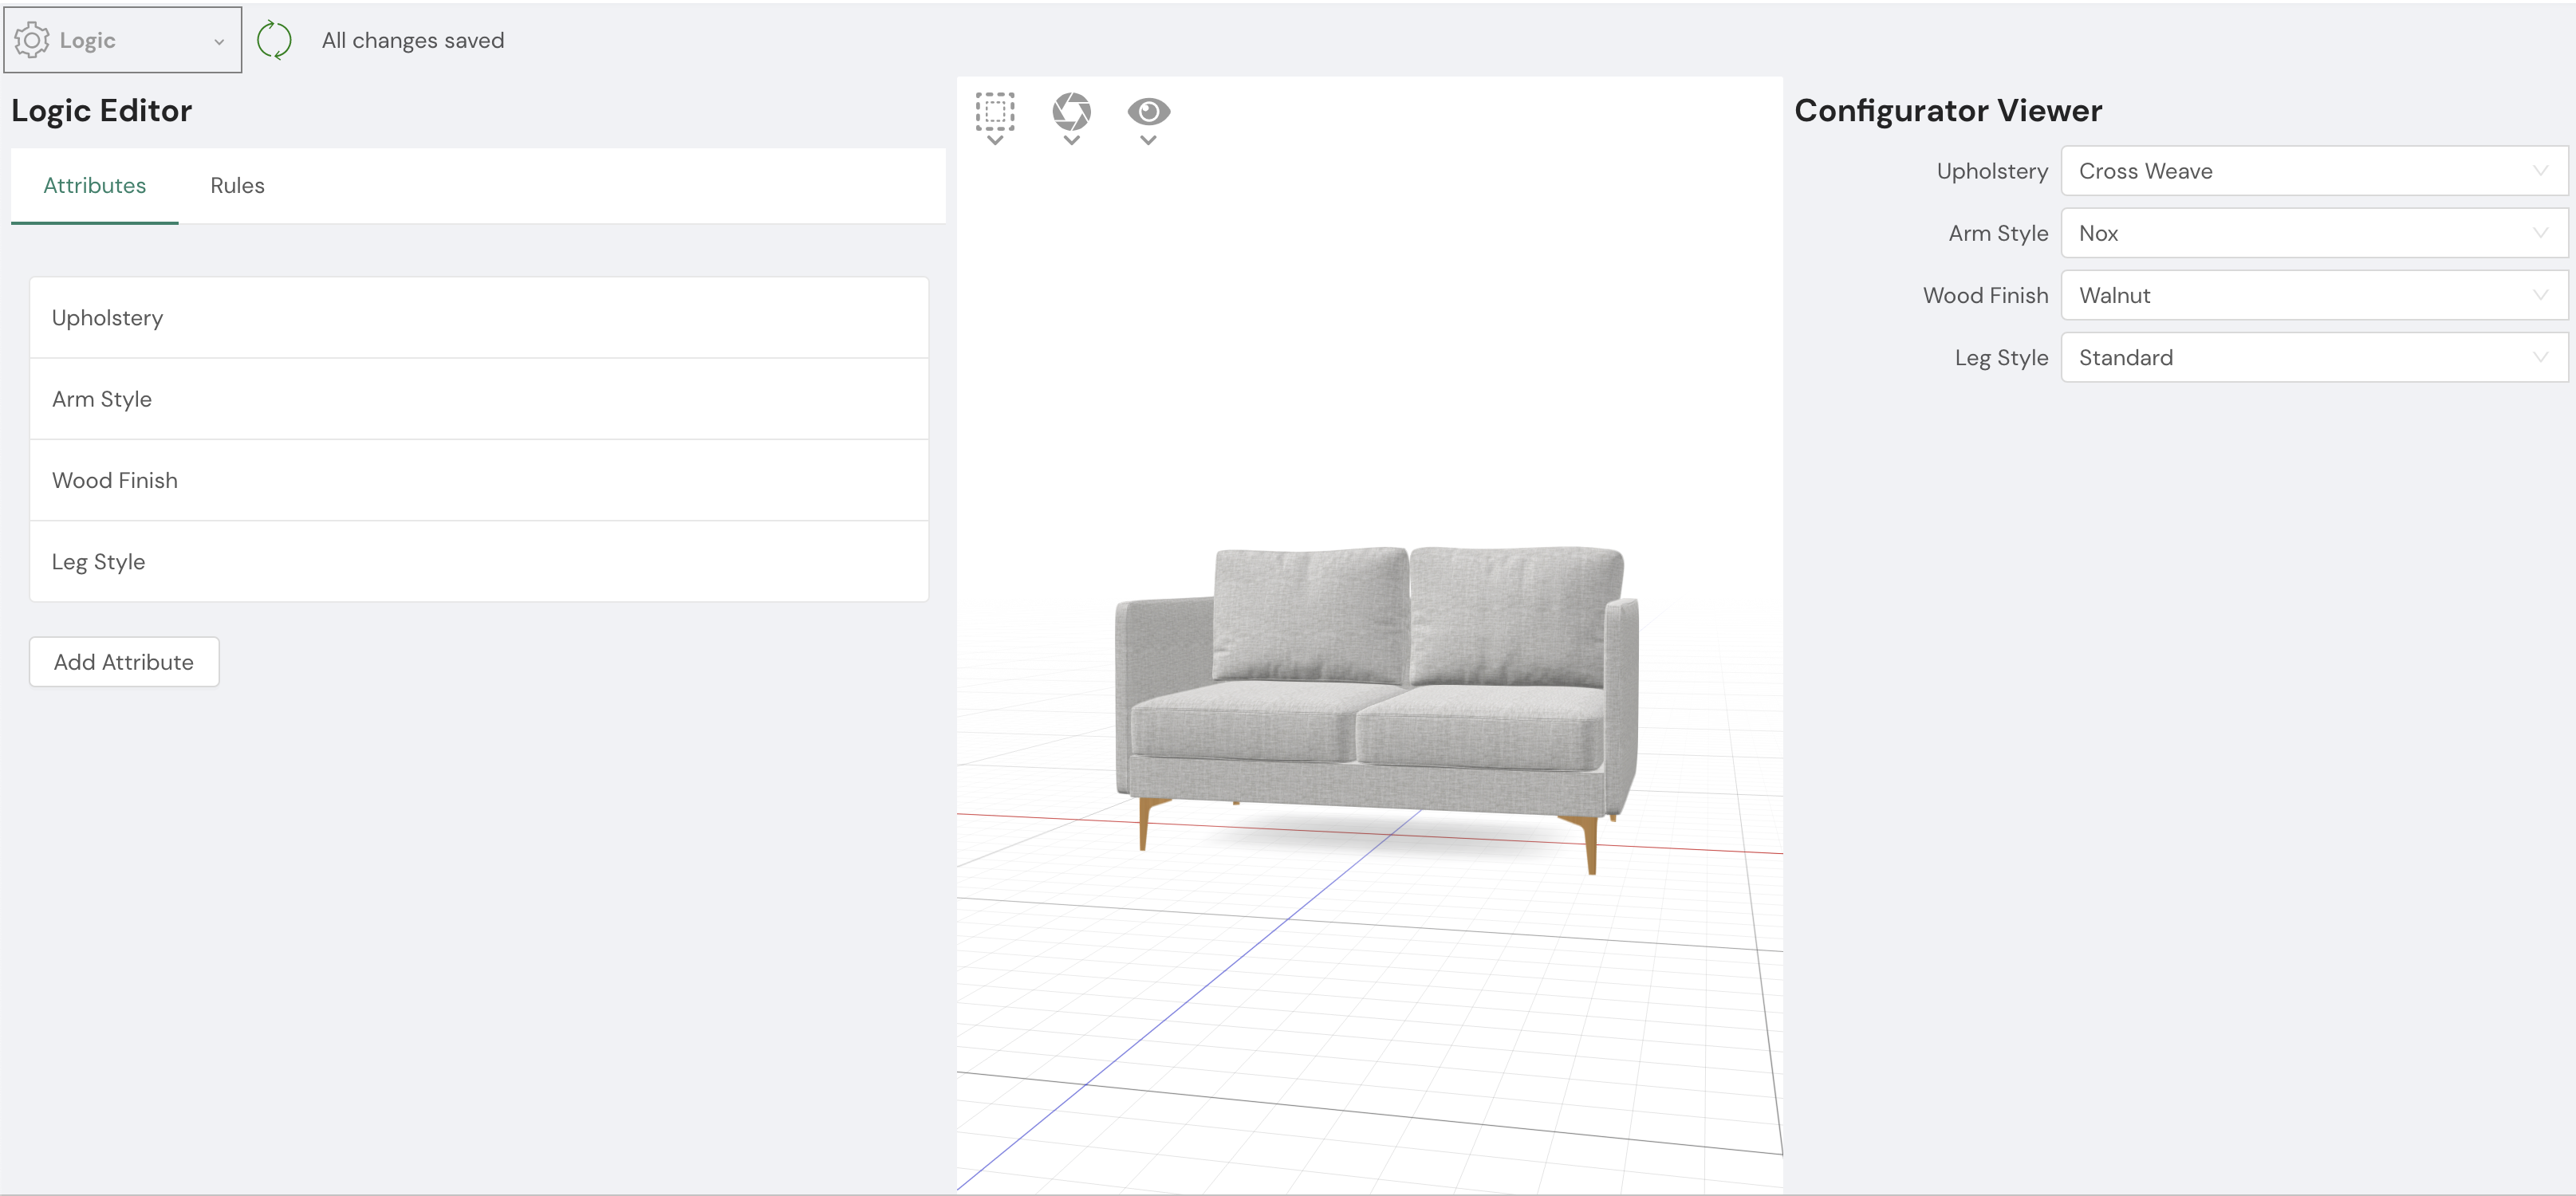
\includegraphics[width=14cm]{images/analysis_threekit-editor.png}
\captionsource{Threekit's Platform's editor}{Threekit Platform Documentation \cite{ThreeKitPlatformDocumentation}}
\label{fig:threekit-editor}
\end{figure}

\begin{figure}
\centering
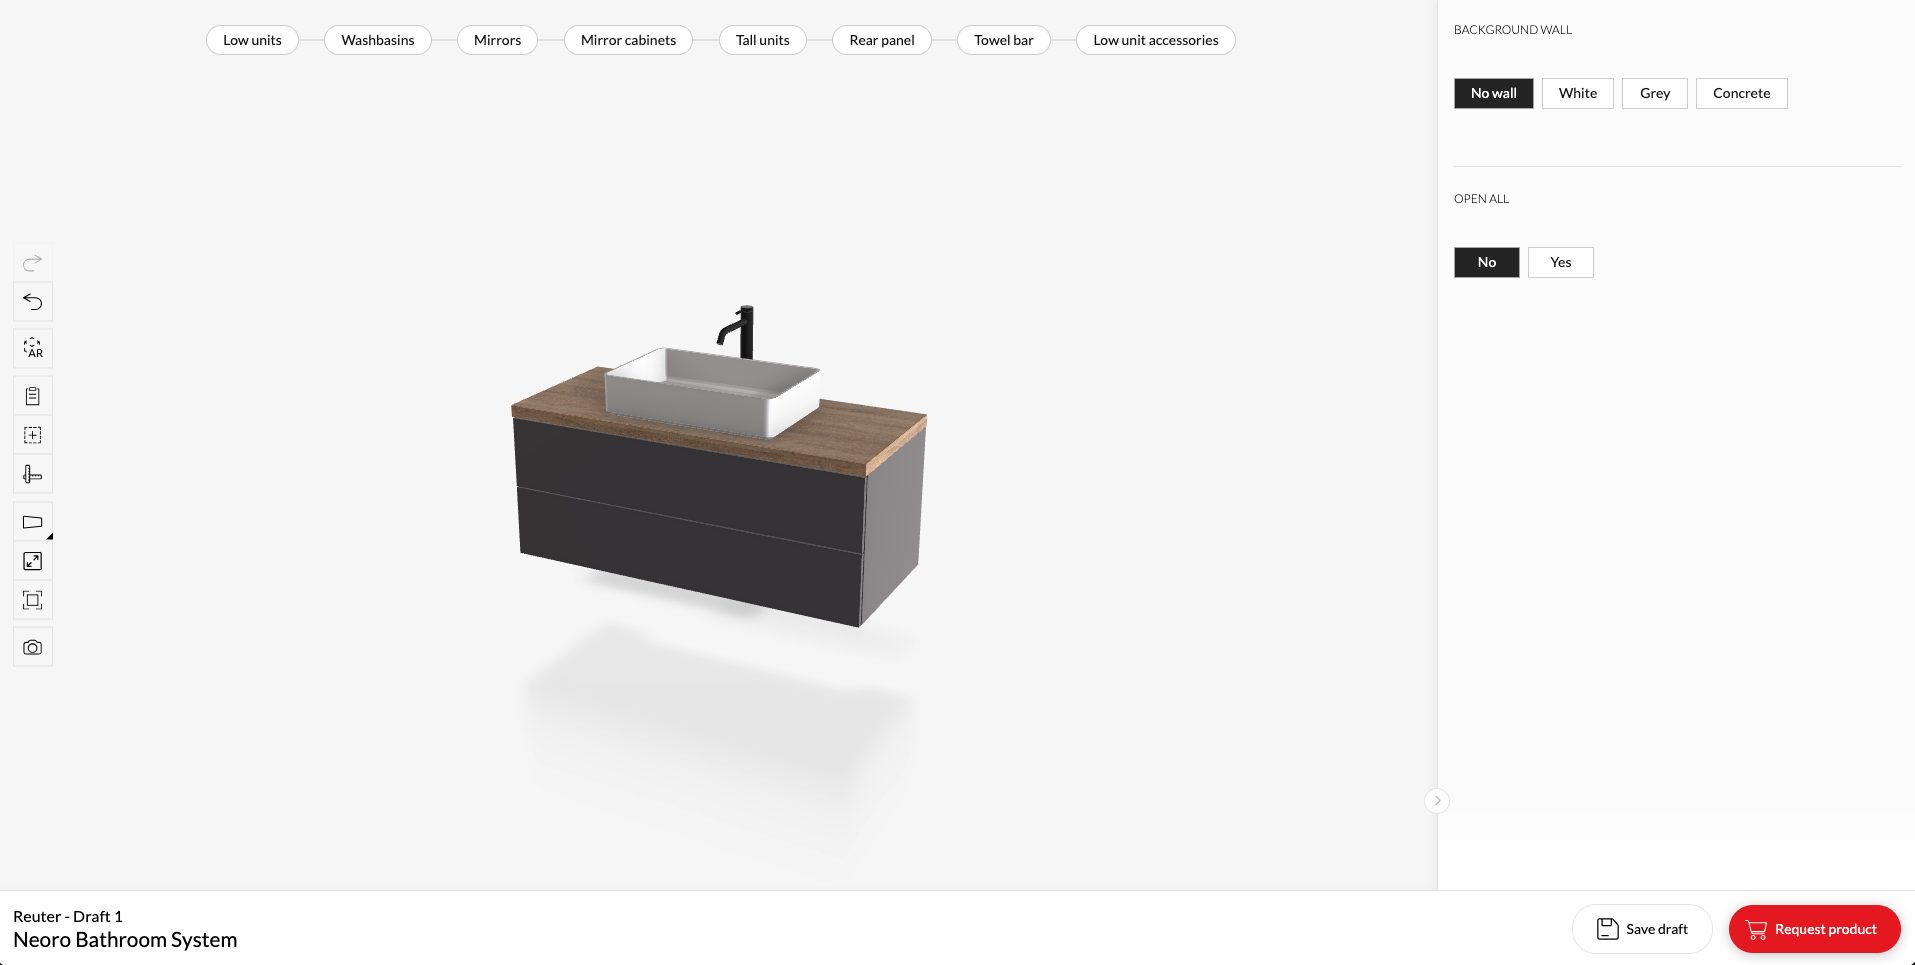
\includegraphics[width=14cm]{images/analysis_roomle.png}
\captionsource{Screenshot of Roomle's Rubens example}{Roomle Demos \cite{RoomleFullLogic}}
\label{fig:roomle}
\end{figure} % include `appendix.tex' from `text/' subdirectory
\chapter{Additional Code Listings} \label{appendix-b}

\begin{listing}
\begin{minted}{typescript}
const renderer = new THREE.WebGLRenderer();
renderer.setSize(window.innerWidth, window.innerHeight);
document.body.appendChild(renderer.domElement);

const scene = new THREE.Scene();

const geometry = new THREE.BoxGeometry(5, 5, 5);
const material = new THREE.MeshBasicMaterial({color: 0xff0000});
const mesh = new THREE.Mesh(geometry, material);
scene.add(mesh);

const camera = new THREE.PerspectiveCamera(
  75,
  window.innerWidth / window.innerHeight,
  0.1,
  1000
);
camera.position.set(10, 10, 10);
camera.lookAt(mesh.position);

renderer.render(scene, camera);
\end{minted}
\caption{Creating and displaying a 3D red cube with Three.js}
\label{listing:threejs}
\end{listing}

\begin{listing}
\begin{minted}{text}
const Component = () => {
    return (
        <Canvas camera={{position: [10, 10, 10]}}>
            <mesh>
                <meshBasicMaterial color="red" />
                <boxGeometry args={[5, 5, 5]} />
            </mesh>
        </Canvas>
    )
}
\end{minted}
\caption{Creating a 3D red cube as a React component with R3F}
\label{lisiting:r3f}
\end{listing}

\begin{listing}
\begin{minted}{typescript}
import { z } from 'zod';

const customSchema = z.number();

type CustomType = z.infer<typeof customSchema>;
\end{minted}
\captionsource{Conversion from Zod schema to TypeScript type}{Adapted from~\cite{Wycliffe2023}}
\label{listing:zod}
\end{listing}

\backmatter % do not remove this command

\todo{Add carrier (online) and dates to websites}
\printbibliography % print out the BibLaTeX-generated bibliography list

\chapter{Concents of the attachment}
% Concents of the attachment

	\dirtree{%
		.1 readme.txt\DTcomment{stručný popis obsahu média}.
		.1 exe\DTcomment{adresář se spustitelnou formou implementace}.
		.1 src.
		.2 impl\DTcomment{zdrojové kódy implementace}.
		.2 thesis\DTcomment{zdrojová forma práce ve formátu \LaTeX{}}.
		.1 text\DTcomment{text práce}.
		.2 thesis.pdf\DTcomment{text práce ve formátu PDF}.
	}
 % include `medium.tex' from `text/' subdirectory

\end{document}
